% chktex-file 44

% DHR: TİO: Tespit İsabet Oranı
% VSM: ZPM: Zafiyet Puanlama Metriği
% SVSM: TZPM: Tekil Zafiyet Puanlama Metriği

\chapter{Giriş}

%% docker nedir
Docker, geliştiricilerin uygulamalarını ve bağımlılıklarını tek bir pakette bir araya getirmelerini sağlayan ve uygulamanın Linux tabanlı herhangi bir ortamda sorunsuz çalışmasını sağlayan bir konteyner teknolojisidir~\autocite{haque2020challenges}. Docker 2013 yılında PyCon'da tanıtıldı ve aynı yılın Mart ayında Solomon Hykes~\autocite{ThefutureofLinuxContainers} tarafından açık kaynaklı hale getirildi. Bu tarihten itibaren, bilişim ve teknoloji (IT) sektöründe oldukça popüler bir endüstri standardı haline gelmiştir. Bunun en büyük nedeni Docker imajlarının geleneksel sanal makinelere ve sanallaştırma teknolojisine göre çeşitli avantajlar sağlamasıdır.

%% Docker'in avantajları
Docker imajlarının kullanıma sunulması modern yazılım geliştirmede  önemli bir başarıdır~\autocite{prado2022}. Docker imajları klasik sanal makinelere göre çeşitli avantajlar sağlamaktadır~\autocite{zhang2018comparative}. Docker imajları sanal makinelere kıyasla çok küçüktür, çünkü sanal makineler tüm işletim sistemini içermekte, ancak Docker imajları sadece uygulama ve uygulamanın çalışması için gerekli olan kütüphaneleri ve bağımlılıkları içermektedir. Docker imajları Linux tabanlı herhangi bir işletim sisteminde çalışabilir çünkü Docker imajların harici bir bağımlılığı yoktur. Birden fazla sanal makine başlatıldığında, her biri için yarı bir Linux çekirdeği oluşturulmaktadır. Bu, sanal makinelerin daha fazla kaynak (RAM ve CPU) kullandığı anlamına gelir. Ancak, docker imajları için durum böyle değildir, çalışan tek bir Linux çekirdeği birden fazla Docker imajını çalıştırmak için yeterlidir.

%% ölçeklenebilirlik
Docker imajları ayrıca mükemmel/gelişmiş ölçeklenebilirlik sağlamaktadır~\autocite{8125559}. Docker Swarm, Hashicorp Nomad, Apache Mesos ve Kubernetes otomatik ölçeklendirme sağladığı için Docker imajlarını ölçeklendirmek sanal makineleri ölçeklendirmekten daha kolaydır. Ayrıca, Docker imajları uygulamaların hızlı ve sürekli dağıtımını sağlar. Konteyner orkestrasyon araçları ile Docker imajları sanal makinelere kıyasla çok hızlı bir şekilde canlıya konuşlandırılabilmektedir.

%% docker imaj istatistikler
Docker imajları bu avantajlar sayesinde son yıllarda popülerlik kazanmıştır. CNCF (Cloud Native Computing Foundation) bulut tabanlı anketine göre 2022 yılında şirketlerin \%45'i canlı (production) ortamda çoğunlukla Docker imajlarını kullanmaktadır. Şirketlerin diğer \%35'i Docker imajlarını canlı ortamlarında kullanmaya başlamıştır. Yine aynı raporda, tüm şirketlerin \%30'u geliştirme ve dağıtım (deployment) süreçleri için bulut tabanlı teknolojilerini kullanmaktadır~\autocite{CNCF2022Report}.

%% https://survey.stackoverflow.co/2023/
StackOverflow 2023 anketine göre, Docker \%51,55 kullanım oranıyla en çok kullanılan geliştirme aracıdır~\autocite{StackOverflow2023Survey}. Benzer şekilde, Kubernetes konteyner orkestrasyon platformu dünya genelindeki kuruluşların \%49'u tarafından kullanılmaktadır~\autocite{CNCF2022Report}. Bu istatistik ve bilgilerden yola çıkarak, Docker imajlarının dünya çapında BT alanında yaygın olarak kullanıldığı sonucuna varabiliriz.

%% explain security risks
Birçok kullanım alanı ve avantajı olmasına rağmen Docker imajları güvenlik riskleri içerebilmektedir. Yamalanmamış Docker imajlarındaki güvenlik açıkları güvenlik için ciddi bir tehdit oluşturur, mali kayıplara ve özel verilerin ifşa edilmesine neden olabilmektedir. Ayrıca, kötü amaçlı veya güncel olmayan konteyner imajları kullanıldığında bu güvenlik riskleri daha da kötüleşebilir. Ek olarak, yanlış yapılandırılmış ve aşırı ayrıcalıklı konteyner imajları, Linux kerneli ve Runc tarafından sağlanan korumaları aşabilir sistemin genel bütünlüğünü tehlikeye atabilmektedir.

CVE-2019{-}5736 gibi keşfedilen bazı güvenlik açıkları, Runc Container Escape zafiyeti nedeniyle konteyner içerisinde çalışan bir uygulamanın yetkisini yükseltmesine ve ana bilgisayar işletim sistemine geçmesine neden olabilmektedir~\autocite{CVE-2019-5736}. Bu güvenlik açığı, saldırganların yönetici (root) olarak bir komut çalıştırmasına, Runc ve kernel tarafından sağlanan güvenlik korumalarını aşmasına ve ana bilgisayar üzerindeki Runc dosyası üzerine veri yazmasına imkan vermektedir.

2017 yılında bir saldırgan Docker Hub'da birkaç kötü niyetli Docker imajı yükledi. Bu imajlar kaldırılmadan önce 5 milyondan fazla kez indirilmiş ve 90.000\$ mali kayba neden olmuştur~\autocite{arstechnicaBackdooredImages}. Benzer şekilde, başka bir saldırgan, Docker Hub'da ``alpine'' ve ``alpine2'' adlı kötü amaçlı imajlar oluşturarak resmi ``alpine'' imajının popülerliğinden yararlandılar. Bu yanıltıcı taktik, geliştiricileri bilmeden zafiyetli imajları kullanmaları için kandırmayı amaçlıyordu~\autocite{trendmicroVinfo}. Saldırganlar bu imajlar ile kripto para madenciliği yaptılar ve zafiyetli Docker sunucularını tespit etmek için masscan~\autocite{masscanrepo} aracı ile network taraması gerçekleştirdiler.

Markus ve arkadaşları, Docker Hub ve diğer özel kayıt defterlerinden 337,171 imajı analiz ettiler ve imajların \%8.5'inin API anahtarları, özel anahtarlar, parolalar vb.\ gibi bilgiler içerdiğini tespit ettiler. 28.621 Docker imajında 52.107 özel anahtar ve 3158 sızdırılmış API anahtarı buldular~\autocite{Dahlmanns_2023}. Bu gizli bilgiler kurumlara büyük bir saldırı yüzeyi açmakta ve verilerin gizliliğini riske atmaktadır.

Yukarıdaki güvenlik olaylarında görüldüğü gibi Docker imajları ile ilgili bazı güvenlik sorunları bulunmaktadır. Bu sorunları çözmek için bazı projeler ortaya çıkmıştır. Chainguard projesi sıfır CVE'li ve zafiyetsiz Docker imajları oluşturmayı hedeflemektedir~\autocite{ChainGuardImages}. Böylece saldırı yüzeyini azaltabilir ve güvenlik riski en aza indirebilir. Docker Hub ayrıca Docker CLI, Docker desktop ve kendi kayıt defteri servisi Docker Hub üzerindeki imaj güvenlik açıklarını belirlemek için Scout projesini başlatmıştır~\autocite{DockerScout}. Benzer şekilde, Redhat kendi Quay imaj kayıt defteri için Clair projesini başlattı~\autocite{QuayRegistry}.

Ancak hala bu çözümlerin etkinlikleri yeterince bilinmemektedir. Bütün bu gelişmelere rağmen konteyner güvenliği yeterince gelişmemiştir. RedHat Kubernetes Güvenliğinin 2023'teki durumu raporunda katılımcıların \%38'i konteyner operasyonlarında güvenlik yatırımlarının yetersiz olduğunu belirtmektedir ve yine aynı raporda katılımcıların \%67'si güvenlik endişeleri nedeniyle bulut tabanlı teknolojilerin benimsenmesini yavaşlatmak zorunda kaldığı vurgulanmıştır~\autocite{RedhatTheStateofKubernetesSecurityin2023}. Bu alanda çeşitli çalışmalar var ancak daha fazla çalışmaya ihtiyaç duyulmaktadır.

Docker imajları konteynerli uygulamaların temelini oluşturduğundan, imajların içindeki yapısal zayıflıklar tüm kurulumu veya uygulamayı saldırıya açık hale getirebilir. Dahası, yazılım geliştirmenin dinamik doğası gereği risk ortamı sürekli değişmektedir. Her gün yeni güvenlik açıkları keşfedilmekte ve bu açıkları düzeltmek için güvenlik güncellemeleri yayınlanmaktadır. Devam eden süreç, yeni keşfedilen güvenlik açıkları hakkında bilgi sahibi olmayı, güvenlik güncellemelerini temel (base) imajlara ve bağımlılıklara derhal uygulamayı ve özelleştirilmiş imajları potansiyel zayıflıklara karşı düzenli olarak taramayı gerektirmektedir.

Güvenlik açığı tespiti, Docker imajların güvenliğini sağlamada kritik bir savunma hattıdır. Bunun için ise öncelikle güvenlik açıklarını güvenilir bir şekilde tespit etmek gerekmektedir. Tez çalışmasının ilk aşamasında, Docker imaj tarama araçları araştırılmış ve analiz edilmiştir. Analiz sonucunda tarama araçlarının etkinlikleri mevcut literatürdeki farklı metrikler kullanılarak değerlendirilmiş ve CVSS risk puanı tabanlı iki metrik önerilmiştir. Önerilen iki metriğin CVSS tabanlı olması sayesinde kritik ve yüksek şiddetli güvenlik açığı tespiti öne çıkarılmıştır.

Tez çalışmasının ikinci aşamasında, popüler Docker imajlarında güvenlik açıklarının zaman içinde nasıl değiştiği incelendi. Docker Hub'dan en çok kullanılan 364 docker imajı belirlendi ve her bir imaj için en az altı ay arayla üç farklı versiyon seçildi ve toplamda 1092 tarama gerçekleştirildi. Tez kapsamında üç zafiyet tarama aracı, Trivy, Grype ve Snyk, kullanıldı ve imajların zaman içinde üç farklı noktada tarandı. Farklı zaman dilimlerindeki sonuçlar analiz edilerek, Docker imajlarının zaman içerisinde güvenlik açığı değişimine ilişkin bilgiler elde edildi.

Araştırmamız en etkili Docker imaj tarama aracının mevcut zafiyetlerin ciddi bir bölümünü tespit edemediğini gösterdi. Benzer şekilde güncellenmemiş Docker imajlarının güncellenmiş olanlarına göre yaklaşık iki katı zafiyet içerdiği görüldü.

\textbf{Tez Çalışmasının Katkıları}

Tez kapsamında literatüre yapılan katkılar şunlardır:

\begin{itemize}
    \item Araştırma, yaygın olarak tanınan üç Docker konteyner tarama aracı olan Trivy, Grype ve Snyk üzerinde gerçekleştirilmiş, bu araçlar çalışma kapsamında önerilen ve literatürde geçen metriklerle kıyaslanmıştır.
    \item Bildiğimiz kadarıyla bu tez, Snyk konteyner tarama aracını değerlendiren ilk çalışmadır.
    \item Docker Hub'da bulunan 439 docker konteyner imajı taranarak büyük ölçekli bir docker imaj değerlendirmesi gerçekleştirildi. İmajların zaman içerisindeki zafiyet değişimlerini tespit etmek için 364 docker imajı seçilmiş ve üç zaman diliminde 1092 docker imajı taranmıştır. % >>> 143 + 101 + 120
    \item Çoğu konteyner imajının yüksek veya orta şiddette güvenlik açığı içerdiği tespit edildi.
    \item Tarama araçlarının etkinliğinin karşılaştırılmasına olanak tanıyan yeni iki değerlendirme metriği önerildi.
    \item Deneysel sonuçlar, birçok imaj tarafından kullanılan işletim sistemi imajlarının dikkatlice seçilmesi gerektiğini ortaya koymuştur. Resmi CentOS imajı gibi bazı işletim sistemi imajlarının bir yıldan uzun süredir güncellenmediği görülmüştür.
    \item Ayrıca CentOS'un en çok güvenlik açığı içeren docker imajı olduğu, alpine ve photon'un ise en güvenli imajlar olduğu gözlemlenmiştir.
    \item CVE-1999{-}0236 gibi 2000 yılından önceki güvenlik açıklarının günümüzde hala keşfedilebildiği gözlemlenmiştir.
    \item Güncellenmiş docker imajlarının saldırı yüzeyini önemli ölçüde azaltabildiği gözlemlenmiştir.
\end{itemize}

\textbf{Tez Çalışmasının Organizasyonu}

Tez aşağıdaki şekilde düzenlenmiştir: Bölüm~\ref{ch:literatur}'de bu alanda yapılan benzer çalışmalar tartışıldı, Bölüm~\ref{ch:methodology}'de tezde kullanılan araştırma metodolojisinin nasıl yürütüldüğü anlatıldı, Bölüm~\ref{ch:arastirma1}'de Docker imaj tarama araçlarının etkinliği çeşitli metrikler ile değerlendirildi, Bölüm~\ref{ch:arastirma2}'de popüler Docker imajlarının zaman içerisindeki zafiyet değişimi araştırıldı ve Bölüm~\ref{ch:kapanis}'da tezde elde edilen bulgular kısaca değerlendirilerek çalışma sonlandırılmıştır.

\chapter{Literatür Taraması}\label{ch:literatur}

Konteyner güvenliği her zaman ilgi çekici bir konu olmuş ve bu alanda çeşitli çalışmalar yapılmıştır. Bunlardan bazıları imaj tarama araçlarını kullanarak konteynerlerin güvenliğini değerlendirmiş, bazıları konteyner imajlarına yönelik tedarik zinciri saldırılarını değerlendirmiş, bazıları konteyner orkestrasyon platformlarını değerlendirmiş ve bazıları Kubernetes ortamındaki CVE'leri değerlendirmiştir. Tez kapsamında bunlardan bazılarına değinilmiştir.

Konteyner imaj tarama araçları, Docker imajlarının güvenlik açıklarını değerlendirmek için çok önemlidir. Uygulamalarının geliştirilmesi ve dağıtımında Docker konteyner imajlarını kullanan birçok kuruluş tarafından tarama araçları kullanılmaktadır. Bu nedenle bazı araştırmacılar özellikle imaj tarama araçlarının etkinliğine odaklanmıştır. Omar ve diğerleri~\autocite{Javed2021} imaj tarama araçlarının efektifliğini incelemiştir. Çalışmalarında, 57 Java tabanlı Docker konteyner imajını değerlendirmişlerdir. İmaj taraması için Clair, Anchore ve Microscanner, statik kod analizi için ise SpotBugs eklentisini kullanmışlardır. En iyi tarama aracının tüm güvenlik açıklarının \%34'ünü gözden kaçırdığını tespit etmişlerdir. Çalışmalarında tespit edilen zafiyet sayısına bağlı tespit isabet oranı (Detection Hit Ratio) isminde bir metrik önermişlerdir. M. Varun ve ark.~\autocite{Varun2023} araştırmaları için Trivy ve Grype imaj tarama aracını kullanmıştır. Altı Docker imajının (Ubuntu, Python, Alpine, Consul ve Postgres) taranması yoluyla temel olarak Trivy ve Grype araçlarını karşılaştırmışlardır. Bu çalışmada, Grype'ın verimliliği Trivy Güvenlik Açığı Veritabanı ile birleştirilerek artırılmıştır. Shay vd.~\autocite{UBCIS} imaj tarama araçlarını değerlendirmiştir. Çalışmalarında 3 Docker imajını (debian:10.2, alpine:3.9.4, ubuntu:18.04) 3 imaj tarama aracı (Trivy, Anchore ve Clair) kullanarak taramışlardır. Çalışmalarında F-Skor formülüne dayanan bir metrik kullandılar. Daha sonra yanlış pozitifleri bulmak için her bir güvenlik açığını manuel olarak incelediler.

Bulut güvenliği öncelikle Docker imajlardaki güvenlik açıklarının tespit edilmesine dayanmaktadır. Bu nedenle bazı araştırmacılar Docker imajlarındaki güvenlik açıklarına odaklanmıştır. Katrine ve ark.~\autocite{VulnerabilityAnalysisof2500DockerHubImages}'da güvenlik açığı taramasına dayalı olarak Docker Hub imajlarındaki zafiyetleri incelemiştir. Çalışmalarında 2500 docker konteyner imajını incelediler ve güvenlik açıklarını bulmak için Anchore konteyner tarama aracını kullandılar. Sertifikalı (verified) imajların \%82'sinde en az bir yüksek veya kritik güvenlik açığı bulunduğunu keşfettiler. Markus ve ark.~\autocite{Dahlmanns_2023} Docker Hub ve diğer kayıt defterlerinden 330.000'den fazla imajı incelemiştir. Docker imajlarının \%8,5'inde parolalar, özel anahtarlar ve API anahtarları da dahil olmak üzere gizli bilgilerin bulunduğunu keşfettiler. Araştırmacılar Docker imajlarında 52.107 özel anahtar ve 3158 sızdırılmış API sırrı tespit etmiştir. Ancak, imaj güvenlik açıklarına değil, yalnızca gizli bilgilerin tespitine odaklandılar.

Tehdit modellemesi, herhangi bir sistemdeki çeşitli güvenlik açıklarını ve tasarım hatalarını tespit etmek ve önlemek için çok önemlidir. Ann ve ark.~\autocite{WONG2023103140}, STRIDE tehdit modelleme çerçevesini kullanarak önce tehdit modellemesi yaparak konteyner güvenliğini incelemişlerdir. STRIDE kullanarak her bir sistem bileşenindeki güvenlik açıklarını tespit etmişler ve ardından bir anket gerçekleştirmişlerdir.

Docker imajlarındaki güvenlik açıkları zaman içinde değişmektedir. Yeni güvenlik açıkları keşfedilmekte ve güvenlik güncellemeleri sürekli olarak yayınlanmaktadır. Alan ve ark.~\autocite{Mills2023} 380 docker imajını analiz ederek bir çalışma gerçekleştirmiştir. 380 docker imajını 3 farklı kategoride analiz etmişlerdir: Resmi, doğrulanmış ve açık kaynak. Çalışmalarının yürütülmesini üç aşamaya ayırmışlardır. Bu yöntemle zaman içinde duyarlılıktaki değişiklikleri gözlemlediler. Tez kapsamında, Docker imajlarının güvenliği için benzer bir yaklaşım kullanılmıştır.

Bu bölümde değinilen çalışmalar konteyner ve imaj güvenliği üzerine yapılan  araştırmaların yalnızca bir bölümünü temsil etmektedir. Literatürde çok sayıda benzer çalışma mevcuttur.

\chapter{Materyal ve Yöntemler}\label{ch:methodology}

Tez kapsamında, Docker imaj tarama araçlarının etkinliği ve Docker imajlarının güvenlik açıkları araştırılmıştır. Güvenlik açıkları ve imaj güvenliği sürekli olarak değişmektedir ve Docker imajlarının güvenlik durumunun zaman içerisinde nasıl değiştiğini değerlendirmek önemlidir. Bunu yapmak için şu iş akışı takip edildi:

\begin{itemize}
    \item Alt bölüm~\ref{subsec:scanner-tool-selection}'de, bir grup imaj tarama aracı araştırılmış ve seçilmiştir.
    \item Alt bölüm~\ref{subsec:image-selection-strategy}'de Docker Hub'dan üç kategoriden olmak üzere en popüler Docker imajları seçilmiştir.
    \item Alt bölüm~\ref{sec:tarama-islemi}'te seçilen Docker imajlarının nasıl tarandığı ve tarama süreci anlatılmıştır.
    \item Alt bölüm~\ref{sec:DataProcessing}'de tarama sonuçlarının nasıl işlendiği açıklanmıştır.
\end{itemize}

\section{Tarama Aracı Seçim Stratejisi}\label{subsec:scanner-tool-selection}

Docker imajlarını taramak için çok sayıda araç online olarak bulunabilir. Bazıları ücretsiz, açık kaynak kodlu ve Github/Gitlab üzerinden erişilebilirken, diğerleri ticari olarak satılmaktadır. İlk olarak, Github'dan başlanarak diğer sitelerde, bloglarda~\autocite{TechbeaconDockersecurity}~\autocite{5opensourcetools}~\autocite{geekflare11Container} imaj tarama araçları araştırılmıştır. İlk araştırmadan sonra, tarama araçları kullanılabilirlik, popülerlik, güncellik ve fiyatlandırma temelinde değerlendirildi. Mevcut tarama araçları tablo~\ref{tab:scanningtoolstable}'deki gibi listelendi:

\begin{table}
    \centering
    \begin{tabular}{ |c|c|c|c| }
     \hline
        Tarama Aracı & Kullandığı Dil & Geliştirici & Fiyatlandırma \\
        \hline
        Trivy & golang & Aqua Security & Ücretsiz \\
        Grype & golang & Anchore & Ücretsiz \\
        Snyk  & type script & Snyk Security & Ücretsiz \\
        Clair & golang & Redhat & Ücretsiz \\
        Dagda & python & Elias Grande & Ücretsiz \\
        Anchore & golang & Anchore & Ücretli \\
        Aqua Scanner & Golang & Aqua Security & Ücretli \\
        Xray & c & JFrog Xray & Ücretli \\
        Qualys Container Security & & Qualys Security & Ücretli \\
        \hline
    \end{tabular}
    \caption{Docker imajı zafiyet tarama araçları.}\label{tab:scanningtoolstable}
\end{table}

Tez çalışmasında, kurulumu ve kullanımı zor olduğu, basit bir CLI arayüzüne ve iyi bir dokümantasyona sahip olmadığı için Clair hariç tutulmuştur. Dagda (son commit 2021~\autocite{DagdaGithub}) gibi güncel olmayan imaj tarama araçları, güncel güvenlik açıklarını bulamadıkları için hariç tutulmuştur. Snyk tabanlı Docker taraması da doğrudan Snyk kullanıldığı için değerlendirme dışı bırakılmıştır. Ticari araçlar, deneme sürümleri mevcut olmayabileceğinden veya yalnızca sınırlı işlevselliğe sahip olabileceğinden dolayı dahil edilmemiştir. Sonuç olarak, tez için Trivy, Grype ve Snyk tarama araçları seçilmiştir.

\section{Docker İmajlarının Seçim Stratejisi}\label{sec:image-selection-strategy}

Docker Hub üzerinde 3,5 milyondan fazla docker imajı bulunmaktadır~\autocite{VulnerabilityAnalysisof2500DockerHubImages}. Benzer şekilde, Github konteyner kayıt defteri, Quay kayıt defteri, Amazon ECR, Google konteyner kayıt defteri ve özel kayıt defteri gibi diğer kayıt defterlerinde de çok sayıda Docker imajı barındırılmaktadır. Her imajın taranması mümkün ve uygulanabilir değildir. Bu nedenle tez kapsamında Docker Hub'dan indirilme (pull) sayısına göre en popüler Docker imajları seçilmiştir.

Docker imajlarını listelemek için Docker Hub API'si kullanılmıştır. İlk olarak, tüm Docker resmi (official) imajları sorgulandı ve ardından hepsi seçildi. Bazı resmi imajların ``latest'' etiketi kullanmadığını tespit edildi. Bu imajlar için imaj etiketlerini manuel olarak kontrol edildi ve tarama için en yeni ve kararlı etiketi kullanılmıştır. Bazı resmi imajların, ``Library/cheer'' gibi, indirilemediği tespit edildi ve bu imajlar atlandı. OSS (Open Source Software) ve doğrulanmış (verified) imajlar için Docker Hub API'si sorgulandı ve ardından 50 milyondan fazla indirilen imajlar seçildi. Bazı Docker imajlarının da ``latest'' etiketi kullanmadığını tespit edildi ve bu imajların etiketleri resmi imajlarda olduğu gibi seçildi.

Toplamda, Docker Hub'da barındırılan ve Tablo~\ref{tab:secilen-imajlar}'de listelenen en çok kullanılan 439 docker imajı seçildi.

\begin{table}
    \centering
    \begin{tabular}{ |c|c| }
        \hline
        İmaj Kategorisi & Taranacak İmaj Sayısı \\
        \hline
        Library & 169 \\
        Verified & 141 \\
        Open Source & 129 \\
        \hline
    \end{tabular}
    \caption{Tez çalışması için başlangıçta seçilen Docker imajları.}\label{tab:secilen-imajlar}
\end{table}

\section{Tarama İşlemi}\label{sec:tarama-islemi}

Tarama için toplamda 439 olmak üzere çok sayıda docker imajı seçildi. Bu kadar çok sayıda imajı manuel olarak taramak çok uzun zaman gerektirmesinden dolayı mümkün değildir. Sonuç olarak tarama işlemi Python ve shell/bash betikleri ile otomatize edildi. Tarama işlemini otomatikleştirilse bile oldukça zaman almaktadır. Bunun üstesinden gelmek için tarama işlemi bulutta gerçekleştirildi, bir VPS (Virtual private server) sunucusu 2 GB RAM, 2 CPU ve 50GB depolama alanı ile kullanılmıştır.

İlk olarak, Docker Hub'dan imajları indiren, ardından imajları 3 farklı araçla (Trivy, Grype ve Snyk) tarayan ve tarama sonuçlarını JSON dosyaları olarak kaydeden bir shell betiği oluşturuldu. JSON'ı ayrıştırmak ve işlemek kolay olduğu için çıktı formatı olarak JSON seçildi. Daha sonra disk alanından tasarruf etmek için Docker imajı silindi. Bir imaja ait indirme işlemi başarısız olursa, o imaj için tarama atlandı.

İmajları tararken Docker Hub'ın imaj indirmeleri için hız sınırlaması uyguladığı tespit edildi. Anonim kullanıcılar için sınır IP adresi başına 6 saatte 100 imaj indirme iken, kimliği doğrulanmış kullanıcılar için sınır 6 saatte 200 imaj indirme olarak belirlendiği görüldü. Sonuç olarak Docker Hub'a \verb|docker login| komutu ile giriş yapıldı ve kullanılan shell betiğinde hız sınırlaması uygulandı.

Bu işlemlerin sonunda, seçilen tüm Docker imajları başarıyla tarandı ve sonuçları kaydedildi.

\section{Tarama Sonuçlarının İşlenmesi}\label{sec:DataProcessing}

Bir önceki adımda Docker imajlarının nasıl tarandığı belirtildi. Şimdi tarama sonuçlarının CSV dosya formatına dönüştürülmesi gerekmektedir, böylece sonuçlar Python ve Pandas ile işlenebilecek, Mathplotlib ve Seaborn ile görselleştirilebilecektir. İlk olarak, JSON dosyalarını ayrıştırmak için bir Python betiği oluşturuldu, ardından sonuçlardan bazı alanlar seçildi. Seçilen alanlar şu şekilde listelenebilir: tarama aracı, imaj türü (resmi, doğrulanmış veya açık kaynak), imaj adı, Güvenlik Açığı CVE ID'si, paket adı, paket sürümü, zafiyet şiddeti (severity) ve CVSS puanı.

Çoğu alanı seçmek kolaydır, fakat CVSS puanı özel dikkat gerektirmektedir. Öncelikle, her güvenlik açığı bir CVE ID'sine ve CVSS puanına sahip olmayabilmektedir. Bazı güvenlik açıkları CVSS2'ye sahipken, CVSS3'e sahip değildir. Benzer şekilde, bazı güvenlik açıkları CVSS3 puanına sahiptir, CVSS2 puanına sahip değildir. CVE ID'si olmayan güvenlik açıkları tarama sonuçlarından hariç tutuldu. Sonuçların geri kalanı için, mevcutsa CVSS3 puanı, mevcut değil ise CVSS2 puanını seçildi. CVSS sonraki bölümlerde detaylarıyla açıklanmıştır(bakınız bölüm~\ref{subsec:ProposedMetric}). Tarama dosyalarının işlenmesinin ardından tüm sonuçlar tek bir CSV dosyasında toplandı.

Kod dosyaları, veri erişilebilirliği bölümünde (bakınız bölüm~\ref{sec:data-availability}) JSON dosyaları ile birlikte paylaşılmıştır.

\section{Kısıtlar}\label{sec:limitations}

Docker imaj güvenliği üzerine yaptığımız çalışma, Docker imaj güvenliği konusunda değerli bilgiler sunsa da, bazı yapısal kısıtları kabul etmek önemlidir. Bu bölümde, tez çalışması sonuçlarımızı yorumlarken göz önünde bulundurulması gereken bazı temel sınırlamaları ele alacağız.

439 Docker imajı üzerinde yaptığımız analizin tüm Docker imajlarının güvenlik risklerini temsil etmeyebileceğini göz önünde bulundurmak önemlidir. Bu da bulgularımızın daha geniş Docker imajları için değişebileceği anlamına gelmektedir.

Ayrıca, tarama sonuçları değerli olmakla birlikte sınırlamalara sahiptir. Güvenlik açığı veritabanları tamamen güncel olmayabilir ve potansiyel olarak yeni keşfedilen zafiyetleri kaçırabilir. Tarama araçlarının kendileri kusurlu olabilir, yanlış pozitifler (gerçekte olmayan güvenlik açıklarını bildirme) veya negatifler (gerçek güvenlik açıklarını kaçırma) üretebilir. Ayrıca, çoğu tarama aracı tarafından kullanılan statik analiz, çalışma zamanı (runtime) güvenlik açıklarını tespit etmede sınırlamalara sahiptir. Güvenlik, sadece güvenlik açıklarını tespit etmek değildir. Tarama araçları, yanlış yapılandırmaları, önceden kodlanmış gizli bilgileri veya konteyner kaçış zafiyetlerini gözden kaçırabilir.

Dikkate alınması gereken bir diğer sınırlama da Docker imajlarının dinamik yapısıdır. Güncellemeler veya yeni zafiyetlerin ortaya çıkması nedeniyle imajların güvenlik durumları zaman içinde değişebilir. Bu nedenle, tarama sonuçlarının bir imajın mevcut güvenlik durumunu doğru bir şekilde yansıtmasını sağlamayı zorlaştırabilir.

Docker imajı güvenliğinin, analizimizde kullandığımız belirli metriklerin ötesine geçtiğini de göz önünde bulundurmamız gerekir. Güvenliği etkileyebilecek başka birçok faktör vardır, bu nedenle bulgularımız Docker imajlarının tamamını yansıtmayabilir.

Bu kısıtlamalara rağmen, tez çalışmamız Docker imaj güvenliğine ilişkin değerli bilgiler vermektedir. Bu kısıtlamaları kabul ederek, tezde ortaya konulan Docker ekosistemindeki güvenlik riskleri değerlendirilebilir.

\chapter{Araştırma 1}\label{ch:arastirma1}

Docker zafiyet tarama araçları, Docker imajı zafiyetlerinin neden olduğu artan saldırı yüzeyi nedeniyle çok önemlidir. Tarama araçlarının önemi, konteynerli ortamlardaki güvenlik açıklarını proaktif olarak tespit etme, değerlendirme ve ele alma becerilerinde yatmaktadır. Kuruluşlar bu araçları geliştirme ve dağıtım süreçlerine entegre ederek genel güvenlik durumlarını iyileştirebilir ve uygulamalarını ve verilerini daha iyi koruyabilirler~\autocite{sultan2019}.

Docker imajlarında yüksek risk taşıyan güvenlik açıklarını tespit etmek çok önemlidir. Bu güvenlik açıklarını tespit eden tarama araçlarının test edilmesi, yeteneklerini anlamak için gereklidir. Bu bölüm, IT sektöründe yaygın olarak kullanılan tarama araçlarının Docker imajlarındaki güvenlik açıklarını tespit etmedeki etkinliğini değerlendirmeyi ve bu araçları birbirleriyle karşılaştırmayı amaçlamaktadır.

Tez kapsamında, imaj tarama araçlarının efektifliğini değerlendirmek için Docker Hub'dan 439 Docker imajı seçilmiştir (imaj seçim stratejisi detayları için bakınız bölüm~\ref{sec:image-selection-strategy}). Bu imajlar daha sonra Trivy, Grype ve Snyk araçları kullanılarak taranmıştır (daha fazla bilgi için araç detayları bölümüne bakınız~\ref{subsec:scanner-tool-selection}). Tarama sonuçları, araçların etkinlik seviyeleri dikkate alınarak karşılaştırılmıştır.

\section{Değerlendirme Sonuçları}\label{sec:ExperimentalResults}

Değerlendirme sonuçları bölümünde, 439 Docker imajından elde edilen verilerin taranması, depolanması ve analiz edilmesinin ardından bulgularımızın değerlendirmesi sunulmuştur. Değerlendirmede, tarama araçlarının etkinliğinin ve performansının kapsamlı bir incelemesini sağlamak için üç farklı metrik kullanılmaktadır.

\subsection{Değerlendirme Metrikleri}\label{sec:EvaluationMetrics}

Değerlendirme metrikleri bölümünde, tarama araçlarının performansını ve etkinliğini değerlendirilmek için kullanılan nicel metrikler tanıtılmaktadır. Değerlendirmemiz, Docker imaj tarama araçlarının doğruluğunu ve güvenilirliğini değerlendirmek için nesnel metrikler olarak hizmet eden üç farklı metrik kullanmaktadır.

İlk metrik, her bir araç tarafından tespit edilen toplam güvenlik açığı sayısına odaklanmaktadır. Bu metrik, araçların Docker imajlarındaki potansiyel güvenlik tehditlerini tespit etme kapasitesine ilişkin temel bir değerlendirme sağlar.

Kullanılan ikinci metrik ise Javed vd.~\autocite{Javed2021} tarafından önerilen Tespit İsabet Oranı (DHR) yöntemidir. Bu yöntemde, imajlar mevcut tüm tarama araçları kullanılarak taranır ve tespit edilen güvenlik açıkları ortak bir havuzda toplanır. Daha sonra, bu ortak havuzdaki her bir tarama aracı tarafından tespit edilen (Hit) ve gözden kaçırılan (Miss) güvenlik açıklarının sayısı hesaplanır. İsabet ve ıskalama oranları belirlendikten sonra metrik Denklem~\ref{eq:dhr}'e göre hesaplanır. Denklem~\ref{eq:dhr}'de, `Hit' tarama aracı tarafından tespit edilen güvenlik açıklarının sayısını gösterirken, `Miss' ortak havuzda bulunan ancak değerlendirilen araç tarafından gözden kaçırılan güvenlik açıklarının miktarını ifade eder.

\begin{equation}\label{eq:dhr}
    DHR = \frac{Hit}{(Hit + Miss)}
\end{equation}

Yukarıda bahsedilen metrikler sadece güvenlik açığı sayısına odaklanmakta ve güvenlik açığının ciddiyetini göz ardı etmektedir. Bu eksiği ele almak için, tez kapsamında önem derecesine dayalı bir yaklaşım (VSM) bölüm~\ref{subsec:ProposedMetric}'de önerilmiştir.

\subsection{Zafiyet Tarama Metriği}\label{subsec:ProposedMetric}

Güvenlik açığı tarama araçlarını yalnızca tespit sayılarına göre değerlendirmek en etkili yaklaşım olmayabilir. Bu sorunu etkili bir şekilde ele almak için, tespit ettikleri güvenlik açıklarının ciddiyetine ilişkin tarama araçlarının karşılaştırmalı analizini yapmak zorunludur. Bu nedenle tez kapsamında, güvenlik açıklarının ciddiyetine dayalı yeni bir metrik önerilmektedir.

Güvenlik açıklarının önem dereceleri Ortak Güvenlik Açığı Puanlama Sistemine (CVSS) göre kategorize edilmektedir. CVSS, bir güvenlik açığının temel özelliklerini yakalamak ve ciddiyetini yansıtan sayısal bir puan üretmek için bir yol sağlar~\autocite{CVSSMainPage}. Şu anda CVSS'nin 4 versiyonu bulunmaktadır. En son versiyon olan 4.\ versiyon 2023 yılında yayınlanmıştır; ancak mevcut verilerin sınırlı olması nedeniyle bu tez kapsamında kullanılmamıştır. Bunun yerine, CVSS puanlarının sürüm 3 ve sürüm 2'si kullanılmıştır. Her sürüm şiddet ve ciddiyet puanları içerir ve tüm puanlar tablo~\ref{tab:cvss-severity} ve~\autocite{CVSSSpecification}'de belirtildiği gibi nitel derecelendirmelerle eşleştirilebilir.

\begin{table}
    \centering
    \begin{tabular}{ |c|c|c| }
        \hline
        Değerlendirme & CVSS Skoru \\
        \hline
        Yok (None) & 0.0 \\
        Düşük (Low) & 0.1~-~3.9 \\
        Orta (Medium) & 4.0~-~6.9 \\
        Yüksek (High) & 7.0~-~8.9 \\
        Kritik (Critical)  & 9.0~-~10.0 \\
        \hline
    \end{tabular}
    \caption{Niteliksel şiddet derecelendirme ölçeği.}\label{tab:cvss-severity}
\end{table}

Bu tez kapsamında CVSS tabanlı bir Güvenlik Açığı Tarama Metriği (VSM), tarama araçlarını kendi aralarında karşılaştırmak için, keşfettikleri güvenlik açıklarının risk seviyelerini dikkate alarak kullanılmıştır. DHR yöntemine benzer şekilde VSM yöntemi de Hit ve Miss güvenlik açıklarını kullanır. Bir tarama aracının $N$ güvenlik açığı tespit ettiğini ve tüm tarama araçları tarafından tespit edilen tüm güvenlik açıklarından $M$ güvenlik açığını kaçırdığını düşünelim. Her bir güvenlik açığına, $i$'inci güvenlik açığı için $n_i$ ile gösterilen bir CVSS puanı atanır. VSM, Denklem~\ref{eq:vsm} kullanılarak hesaplanabilir:

\begin{equation} \label{eq:vsm}
    VSM = \frac{\sum_{i=1}^{N} n_i}{(N+M) \times 10}
\end{equation}

% In equationn~\ref{eq:vsm}, $VSM$ represents the calculated Vulnerability Scoring Metric. The numerator $\sum_{i=1}^{N} n_i$ denotes the sum of the CVSS scores of all vulnerabilities detected by the scanning tool. The denominator $(N+M) \times 10$ standardizes the metric, guaranteeing that the VSM falls within a range of 0 to 1, making it easier to compare across various scanning tools.
Denklem~\ref{eq:vsm}'de, $VSM$ hesaplanan Güvenlik Açığı Tarama Metriğini temsil eder. Pay $\sum_{i=1}^{N} n_i$ tarama aracı tarafından tespit edilen tüm güvenlik açıklarının CVSS puanlarının toplamını ifade eder. Payda $(N+M)\times 10$, VSM'nin 0 ila 1 aralığında olmasını garanti ederek metriği standartlaştırır ve tarama araçları arasında karşılaştırma yapmayı kolaylaştırır.

% VSM (Vulnerability Scanning Metric) being a DHR-based method, serves as a metric suitable for comparing multiple scanning tools. Essentially, after multiple scanning tools conduct their scans, the Hit ($N$) and Miss ($M$) counts are determined based on the security vulnerabilities gathered in a shared pool. To evaluate security vulnerabilities solely based on their risk levels without the need for these counts, we propose the Singular Vulnerability Scanning Metric (SVSM) as a second metric. The mathematical expression for the SVSM method is provided in Equation~\ref{eq:vsm}.
DHR tabanlı bir yöntem olan VSM, birden fazla tarama aracını karşılaştırmak için uygun bir metrik olarak hizmet vermektedir. Esasen, birden fazla tarama aracı taramalarını gerçekleştirdikten sonra, ortak bir havuzda toplanan güvenlik açıklarına dayalı olarak Hit ($N$) ve Miss ($M$) sayıları belirlenir.

Güvenlik açıklarını bu sayılara ihtiyaç duymadan sadece risk seviyelerine göre değerlendirmek için ikinci bir metrik olarak Tekil Güvenlik Açığı Tarama Metriğini (SVSM) öneriyoruz. SVSM yönteminin matematiksel ifadesi Denklem~\ref{eq:svsm}'de verilmiştir.

\begin{equation} \label{eq:svsm}
    SVSM = (1-e^{-\lambda N}) \frac{\sum_{i=1}^{N} n_i}{N \times 10}
\end{equation}

% In Equation~\ref{eq:svsm}, the average CVSS score is calculated by dividing the sum of CVSS scores by the total number of vulnerabilities. Since the CVSS score ranges from 0 to 10, the results are normalized to a range of 0 to 1 by dividing by 10. In its current form the formula normalizes the average of the security vulnerability scores to a range between 0 and 1. In other words, it calculates an independent value regardless of the number of identified security vulnerabilities. To reflect the number of identified security vulnerabilities in the metric, this value is divided by the total number of security vulnerabilities ($N$). In this case, a SVSM  value closer to 0 indicates a more effective scanning tool.
Denklem~\ref{eq:svsm}'de ortalama CVSS puanı, CVSS puanlarının toplamının toplam güvenlik açığı sayısına bölünmesiyle hesaplanır. CVSS puanı 0 ila 10 arasında değiştiğinden, sonuçlar 10'a bölünerek 0 ila 1 aralığına normalleştirilir. Mevcut haliyle formül, güvenlik açığı puanlarının ortalamasını 0 ile 1 arasında bir aralığa normalleştirmektedir. Başka bir deyişle, tespit edilen güvenlik açığı sayısından bağımsız olarak bağımsız bir değer hesaplamaktadır. Tespit edilen güvenlik açığı sayısını metriğe yansıtmak için bu değer toplam güvenlik açığı sayısına ($N$) bölünür. Lambda değeri zafiyet sayısı arttıkça lambda değeri düşürülerek sayının metrik üzerindeki etkisi artmaktadır. Bu durumda, 1'e yakın bir SVSM değeri daha etkili bir tarama aracına işaret eder.

\section{Araştırma 1 Sonuçları}\label{sec:sonuclar}

Aşağıdaki bölümde önceki bölümlerde önerilen metodolojilerin ve metriklerin uygulanmasından elde edilen sonuçlar sunulmaktadır. Bu sonuçlar, incelenen zafiyet tarama araçlarının etkinliği ve performansı hakkında fikir vermektedir. Kapsamlı analiz ve yorumlama ile, güvenlik açıklarının belirlenmesi ve değerlendirilmesinde her bir tarama aracının güçlü ve zayıf yönlerine ışık tutmak amaçlanmıştır.

\subsection{Zafiyet Tespit Sayılarına Göre Sonuçlar}\label{subsec:ResultsByDetectionCounts}

Araçların karşılaştırılmasına, tespit edilen güvenlik açıklarının incelenmesiyle başlanabilir. Bu metrik yalnızca güvenlik açıklarının sayısını dikkate alır ve önemli bilgiler sunar. Şekil~\ref{fig:fig1}'de bu bulgular görsel olarak temsil edilmektedir.

Şekil~\ref{fig:fig1}-a'da, her bir tarama aracının tüm imajlarda CVE ID'lerine göre bulduğu benzersiz güvenlik açığı sayısı ve tüm tarama araçlarının bulduğu toplam benzersiz güvenlik açığı sayısı verilmiştir. Tüm imajların taranması sonucunda bulunan benzersiz güvenlik açığı sayıları incelendiğinde, Grype'ın en yüksek sayıda güvenlik açığı tespit ettiği görülmektedir. Trivy çok az bir farkla Grype'ı yakından takip etmekte, onu da Snyk izlemektedir. Bu sayılar, 439 imajın taranmasının ardından bulunan farklı CVE-ID değerlerine sahip benzersiz güvenlik açıklarının sayısını temsil etmektedir (ayrıntılar için Tablo~\ref{tab:secilen-imajlar}'a bakın). Buna göre, tüm imajların tüm araçlarla taranması toplam 8752 benzersiz güvenlik açığı ortaya çıkarmıştır.

Güvenlik açıkları ayrıca imaj türü, imaj adı, paket adı ve paket sürümüne göre etiketlenmiştir. Bu etiketlemenin ardından, her bir araç tarafından bulunan toplam güvenlik açığı sayısı ve tüm araçların toplamı Şekil~\ref{fig:fig1}-b'de gösterilmektedir. Şekil~\ref{fig:fig1}'de verilen grafikler karşılaştırıldığında, Grype tekil güvenlik açığı sayısı bakımından önde gelirken, Trivy imajlarda bulunan toplam güvenlik açığı sayısında önemli ölçüde üstünlük sağlamaktadır. Daha fazla açıklık getirmek gerekirse, Trivy'nin 439 docker imajını taradıktan sonra bulduğu farklı güvenlik açığı sayısı 6779 iken, Trivy'nin tüm imajlarda bulduğu toplam güvenlik açığı sayısı 111865'tir. Benzer bir durum diğer araçlar için de geçerlidir. Grafikler arasında Trivy ve Grype araçları arasındaki sıralama değişse de Snyk her iki grafikte de sürekli olarak son sırada yer almaktadır.

\begin{figure}
	\centering
	\begin{subfigure}[]{\linewidth/2}
		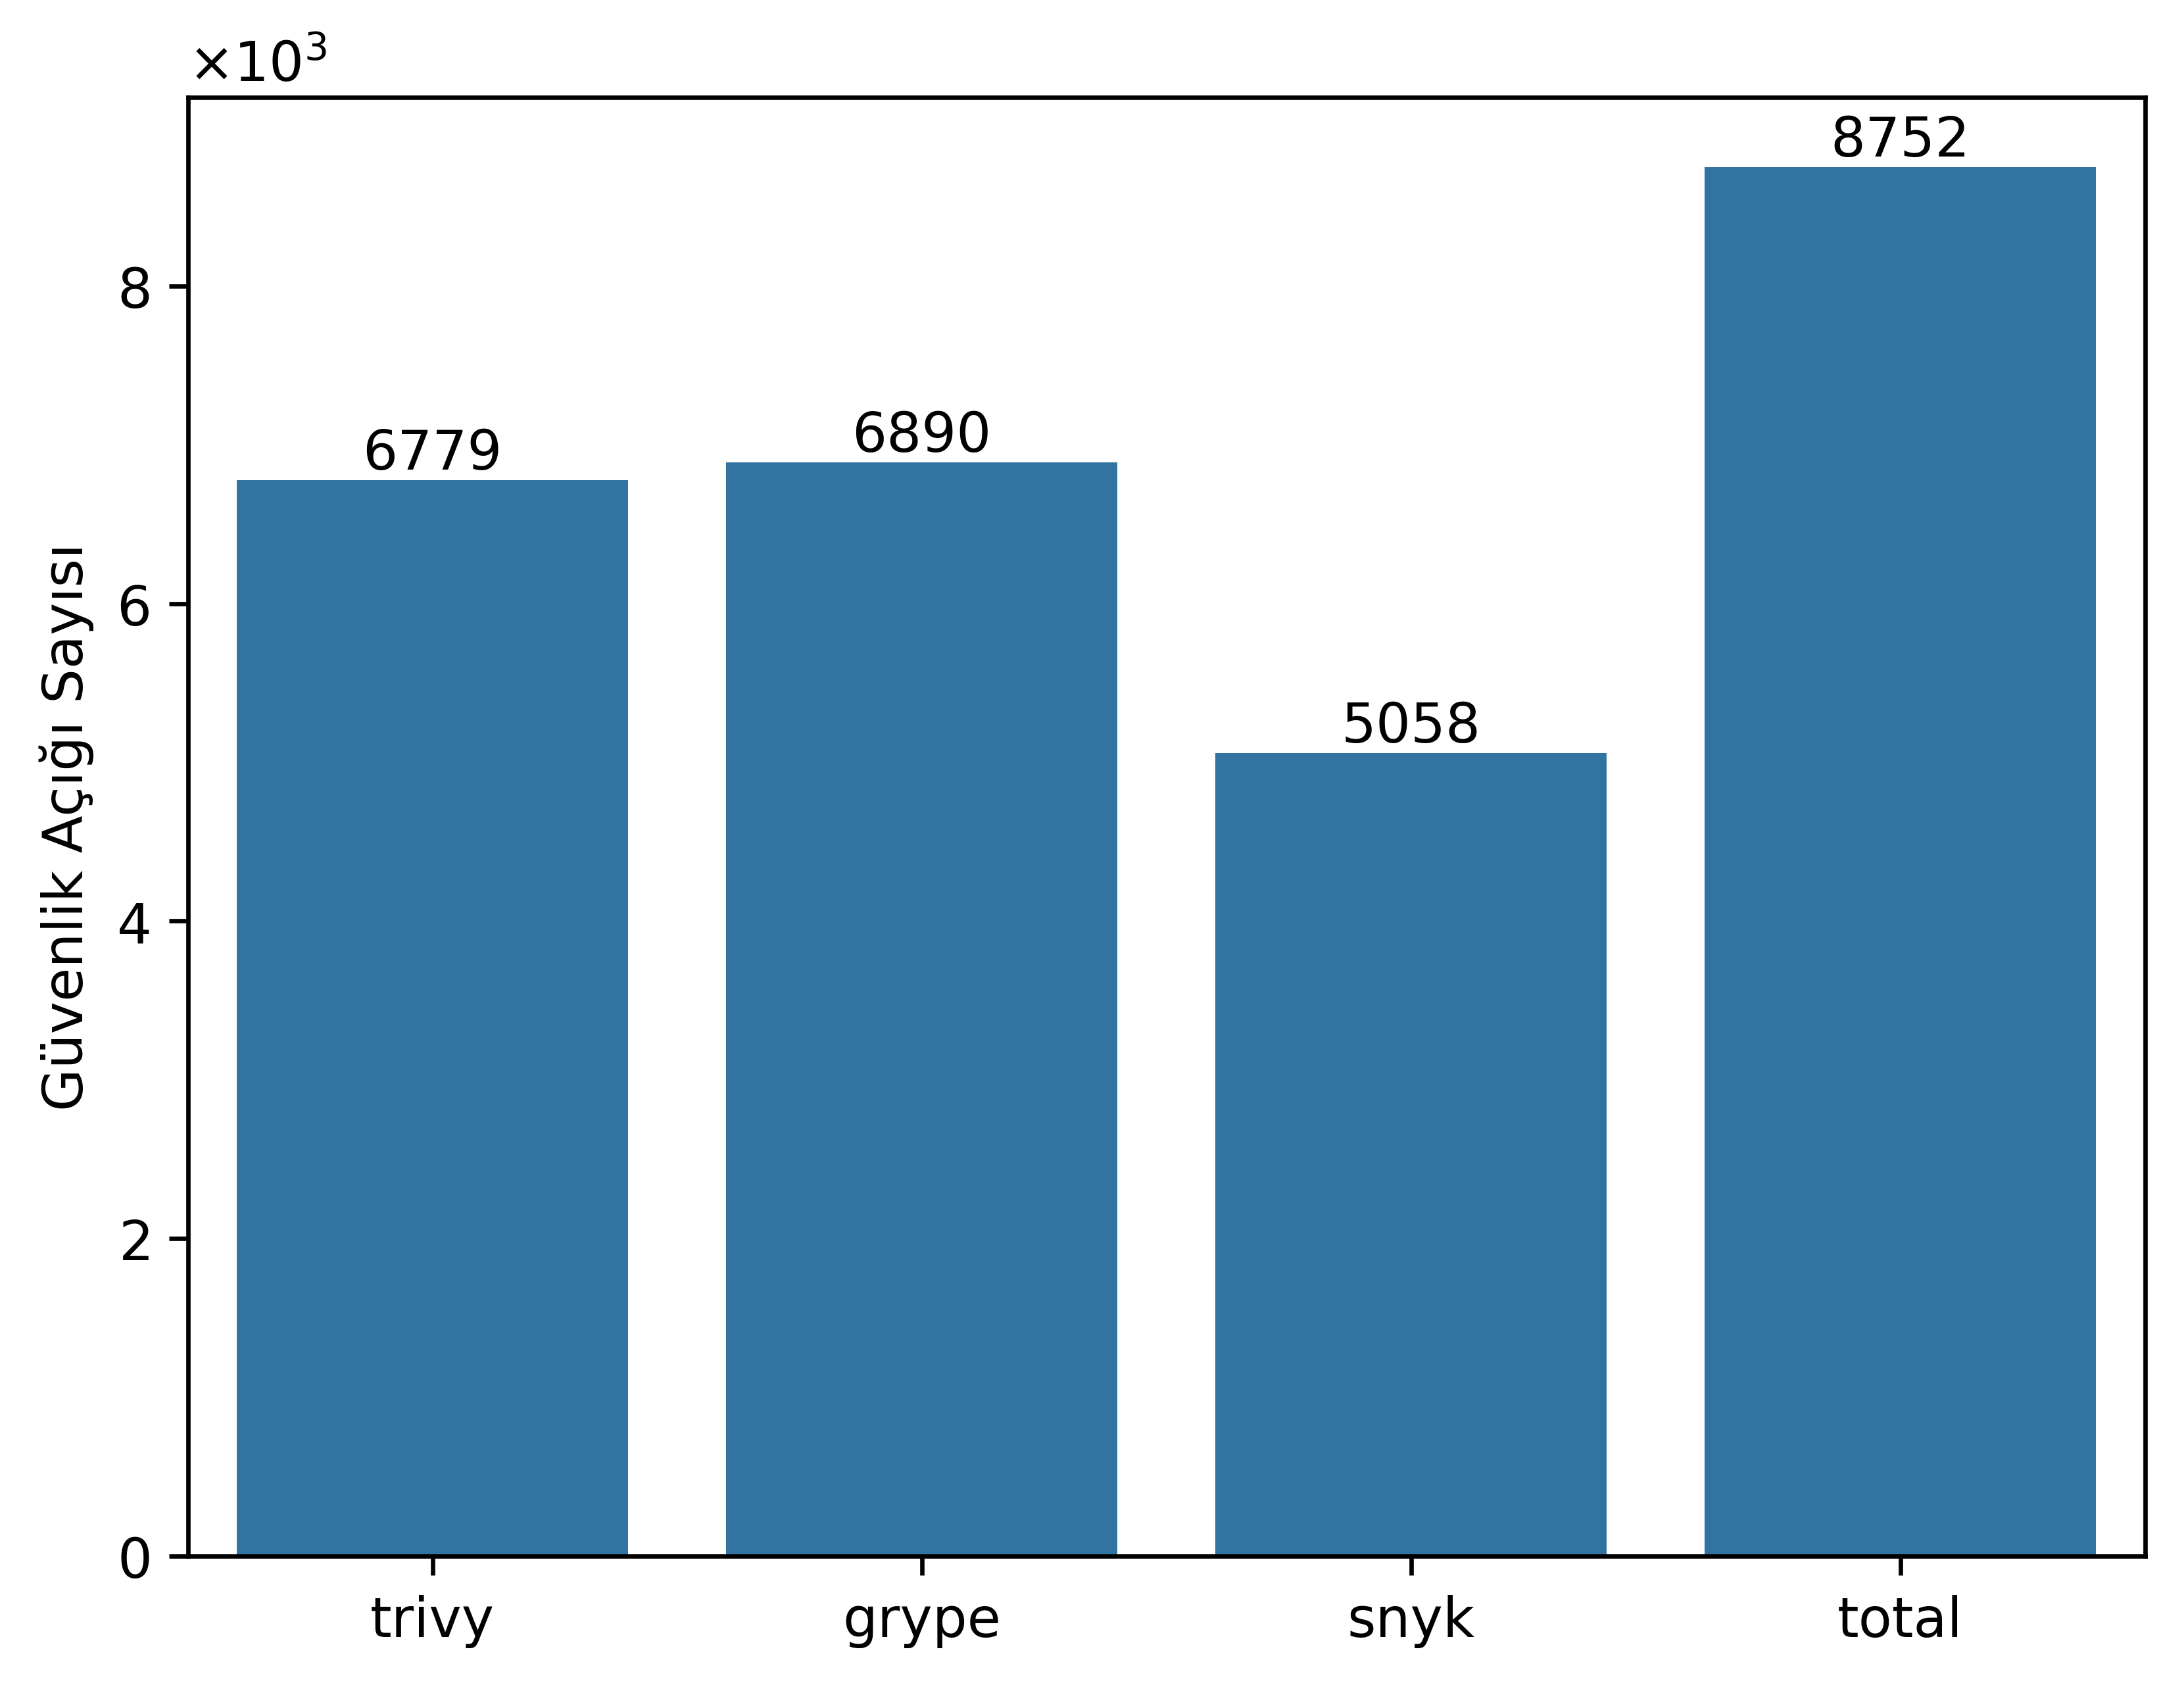
\includegraphics[width=\linewidth]{images/s1/vulCountsUniq.png}
		\caption{Eşsiz zafiyet sayıları}\label{fig:vulCountsUniq}
	\end{subfigure}%
	\begin{subfigure}[]{\linewidth/2}
		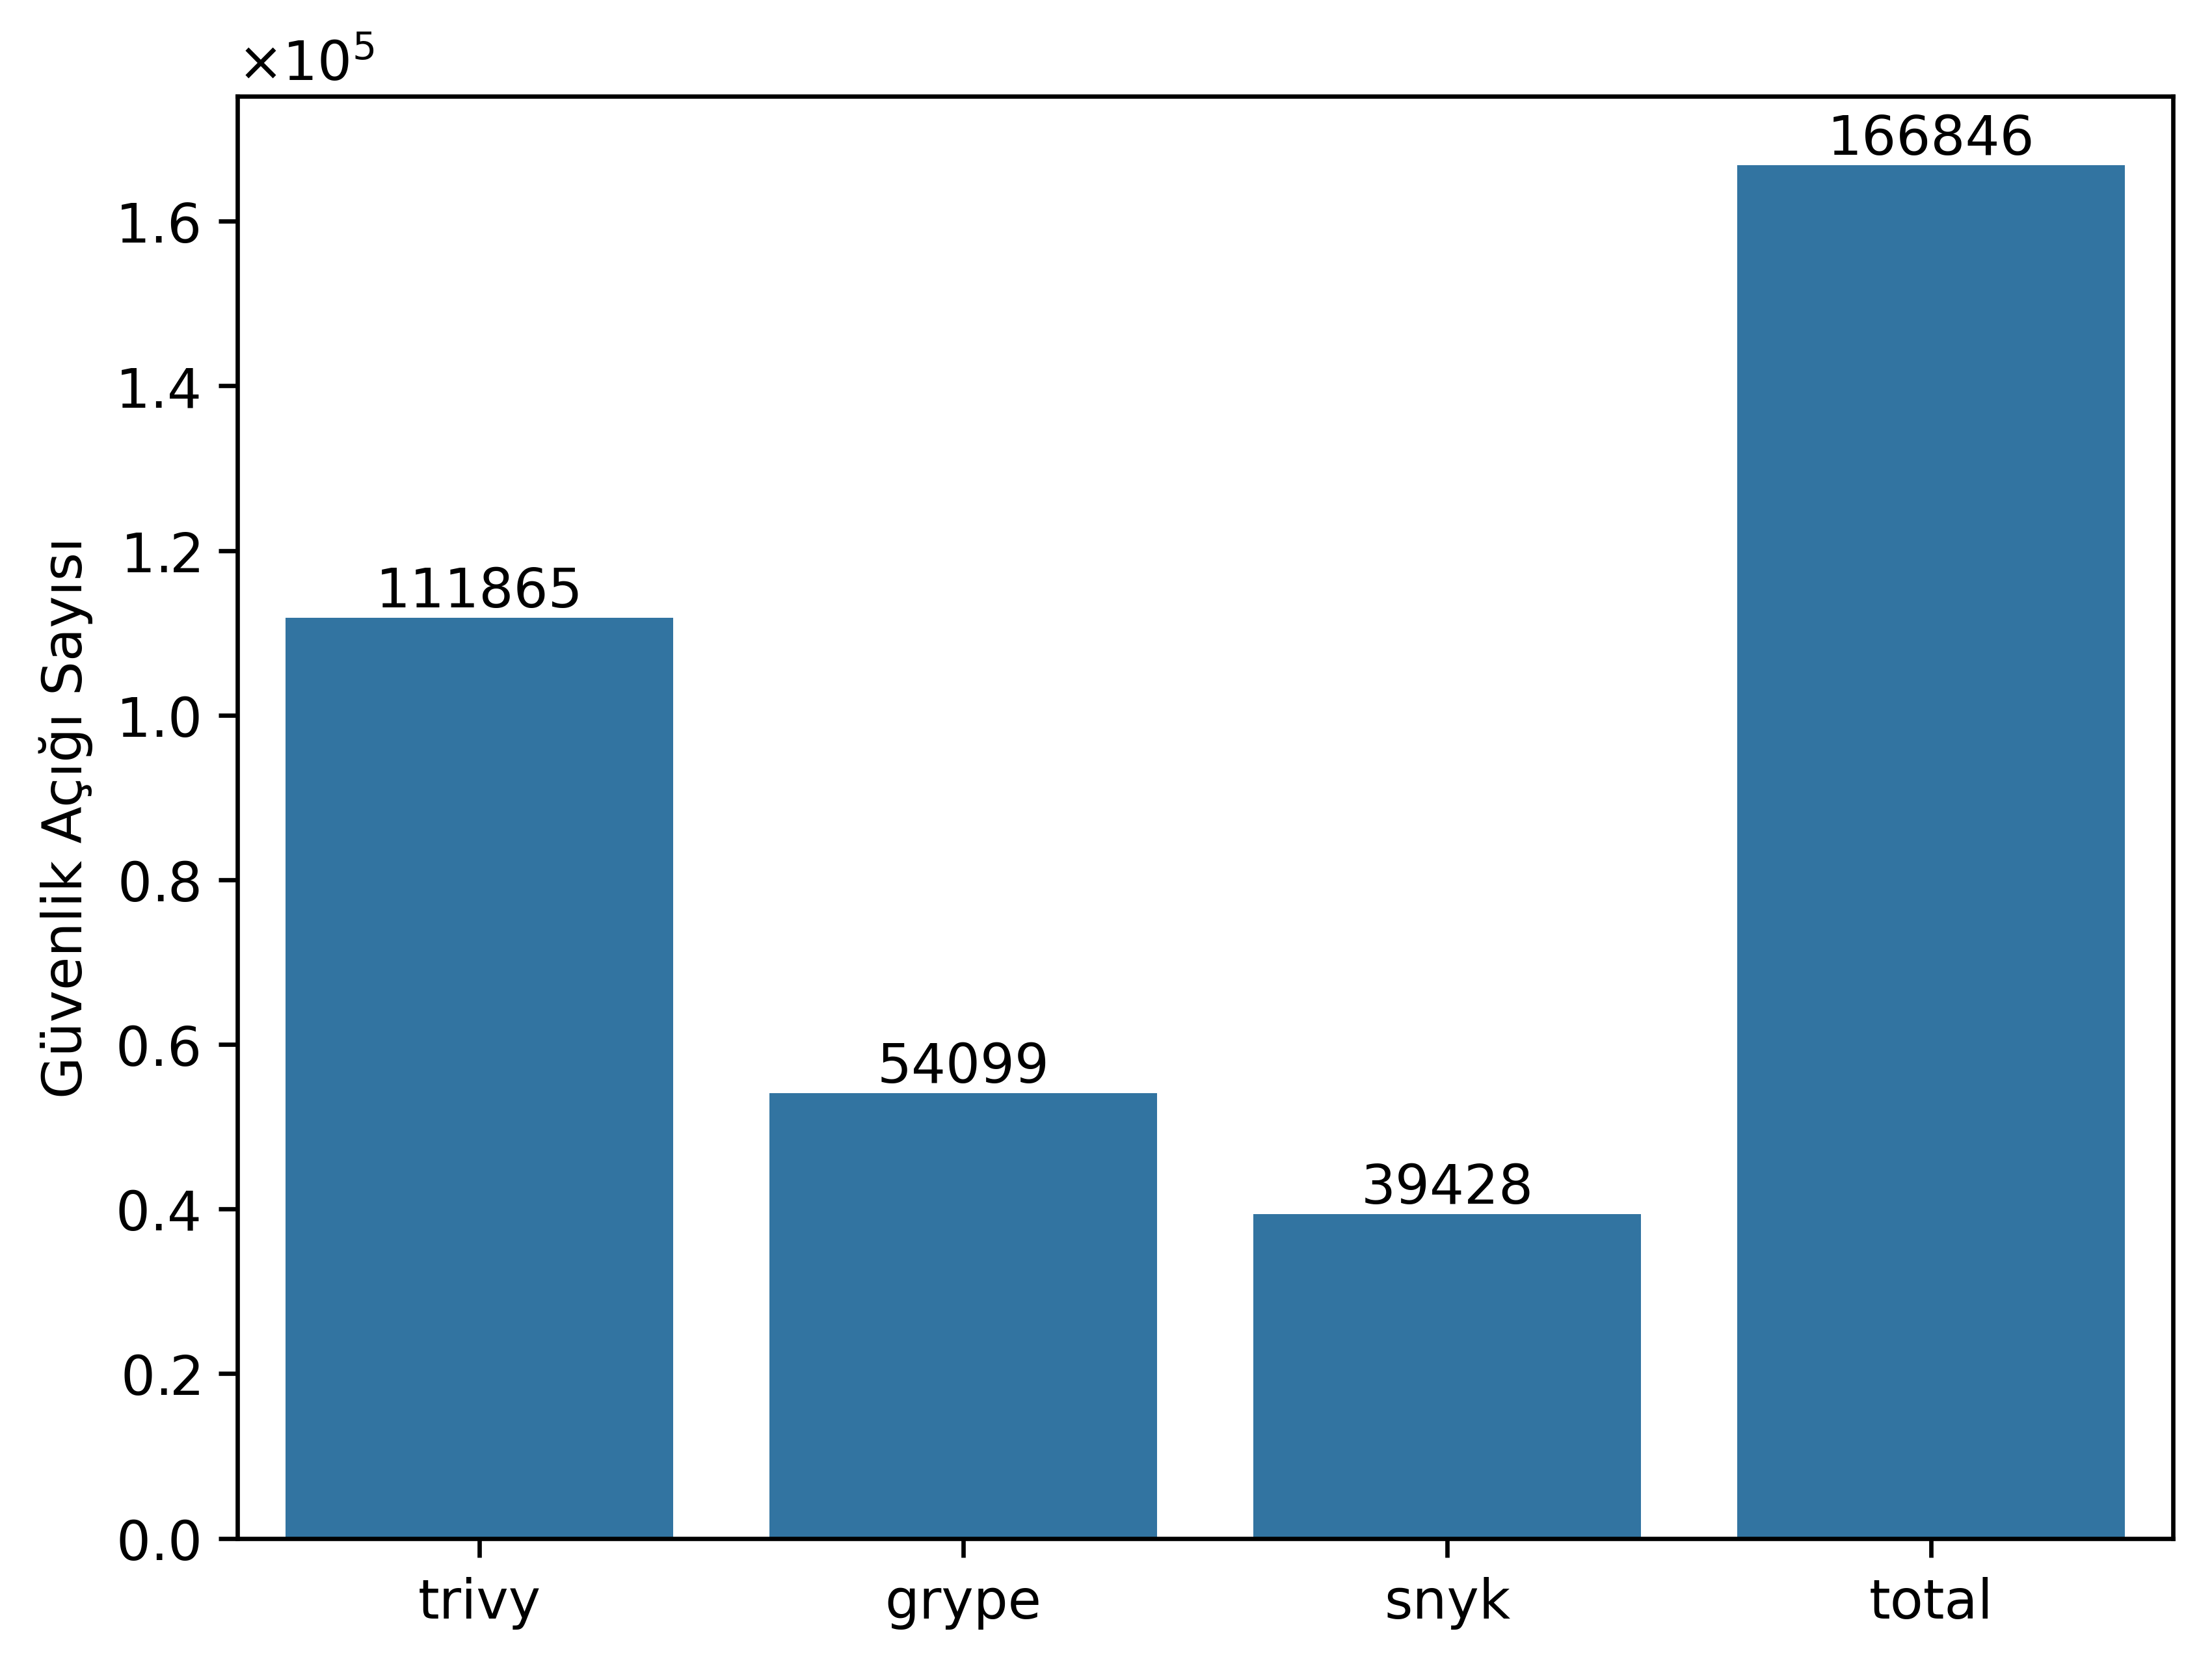
\includegraphics[width=\linewidth]{images/s1/vulCountsAll.png}
		\caption{Zafiyet sayıları}\label{fig:vulCountsAll}
	\end{subfigure}

	\caption{Her bir araç tarafından tespit edilen eşsiz ve toplam güvenlik açığı sayıları.}\label{fig:fig1}
\end{figure}

Şekilde görüldüğü gibi~\ref{fig:fig1} Trivy en iyi performansı göstermektedir, Grype ikinci, Snyk ise son sırada yer almaktadır.

Tarama araçlarının benzersiz ve toplam güvenlik açığı tespit sayılarının kesişim diyagramları sırasıyla Şekil~\ref{fig:fig2}-a ve Şekil~\ref{fig:fig2}-b'de Venn diyagramlarında gösterilmiştir. Şekil~\ref{fig:fig2}-a'daki Venn diyagramına bakıldığında, tüm araçlar tarafından tespit edilen ortak eşsiz güvenlik açığı sayısının 4171 olduğu görülebilir. Bu sayı toplam tespit edilen güvenlik açığı sayısının (8752) yarısından azdır. Bu, docker imajlarındaki güvenlik açıklarının birden fazla araç tarafından daha iyi kapsanabileceğini göstermektedir. Benzer bir sonuç, Şekil~\ref{fig:fig2}-b'de verilen ve tüm imajlar tarandıktan sonra bulunan güvenlik açıklarını gösteren Venn diyagramı incelenerek de çıkarılabilir.

\begin{figure}
	\centering
	\begin{subfigure}[Figure A]{\linewidth/2}
		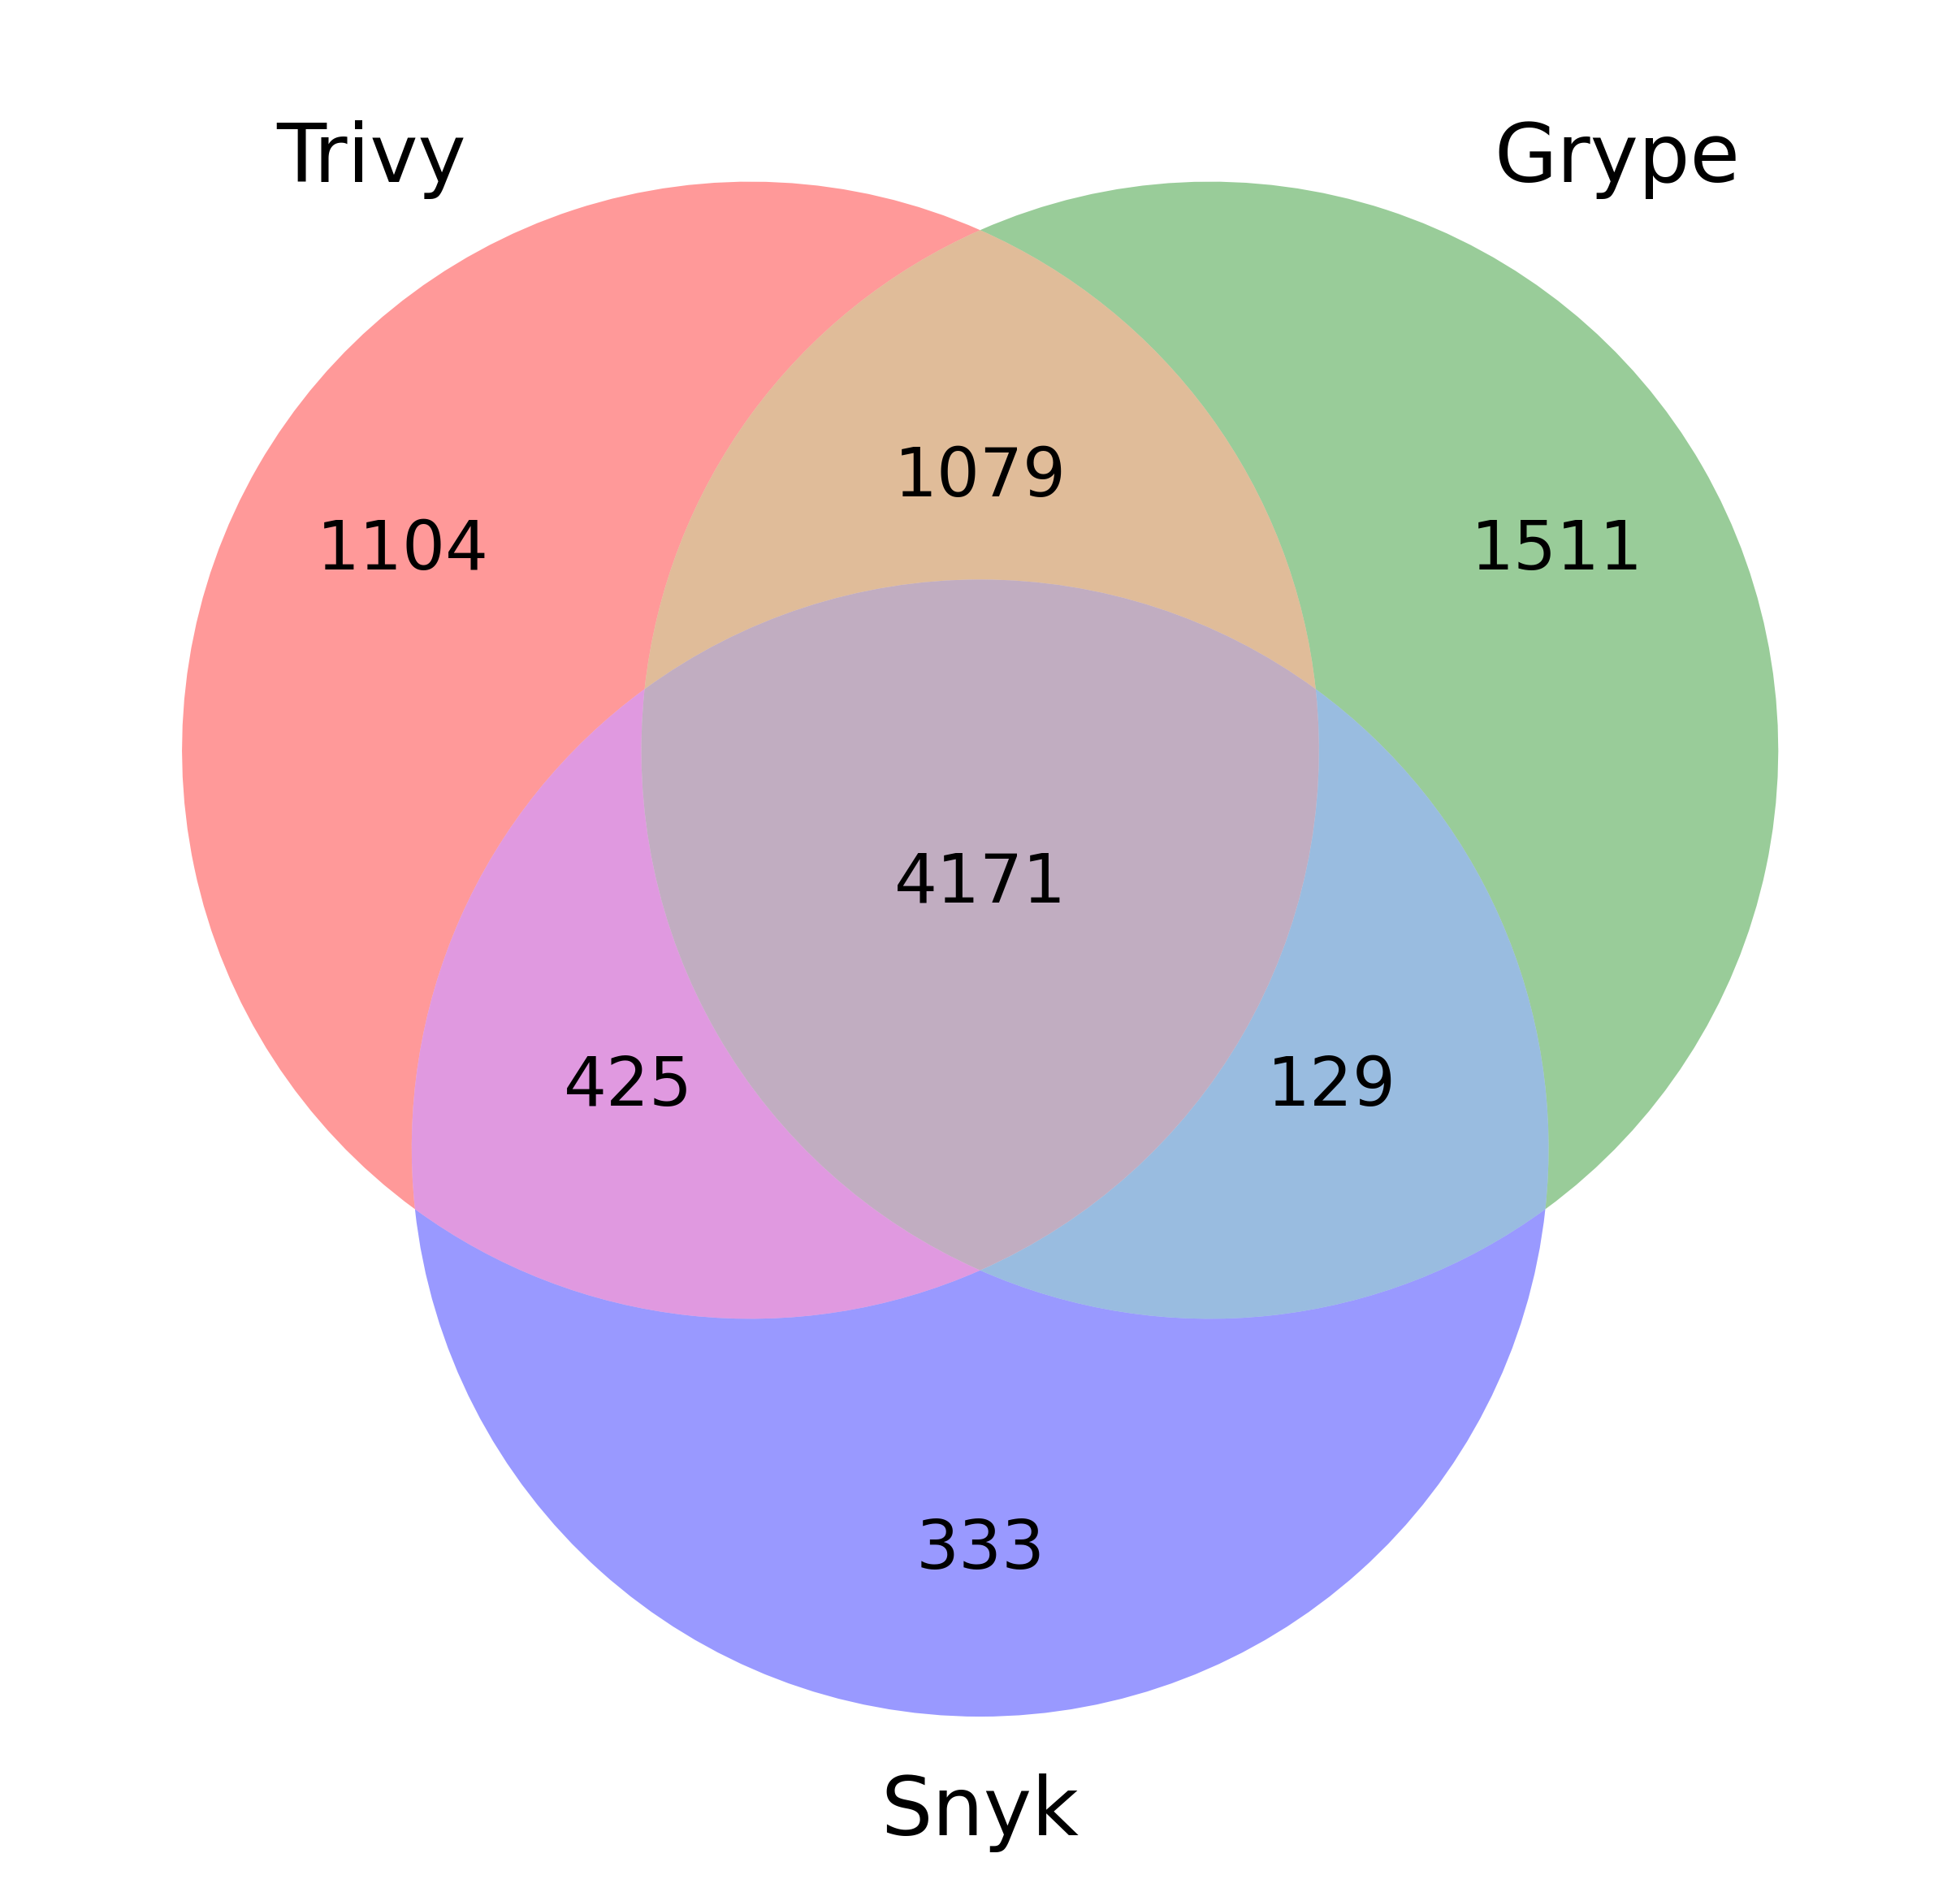
\includegraphics[width=1\linewidth]{images/s1/vulCountsVennUniq.png}
		\caption{Eşsiz zafiyetlere ait venn diyagramı.}\label{fig:vulCountsVennUniq}
	\end{subfigure}% vertical
	\begin{subfigure}[Figure A]{\linewidth/2}
		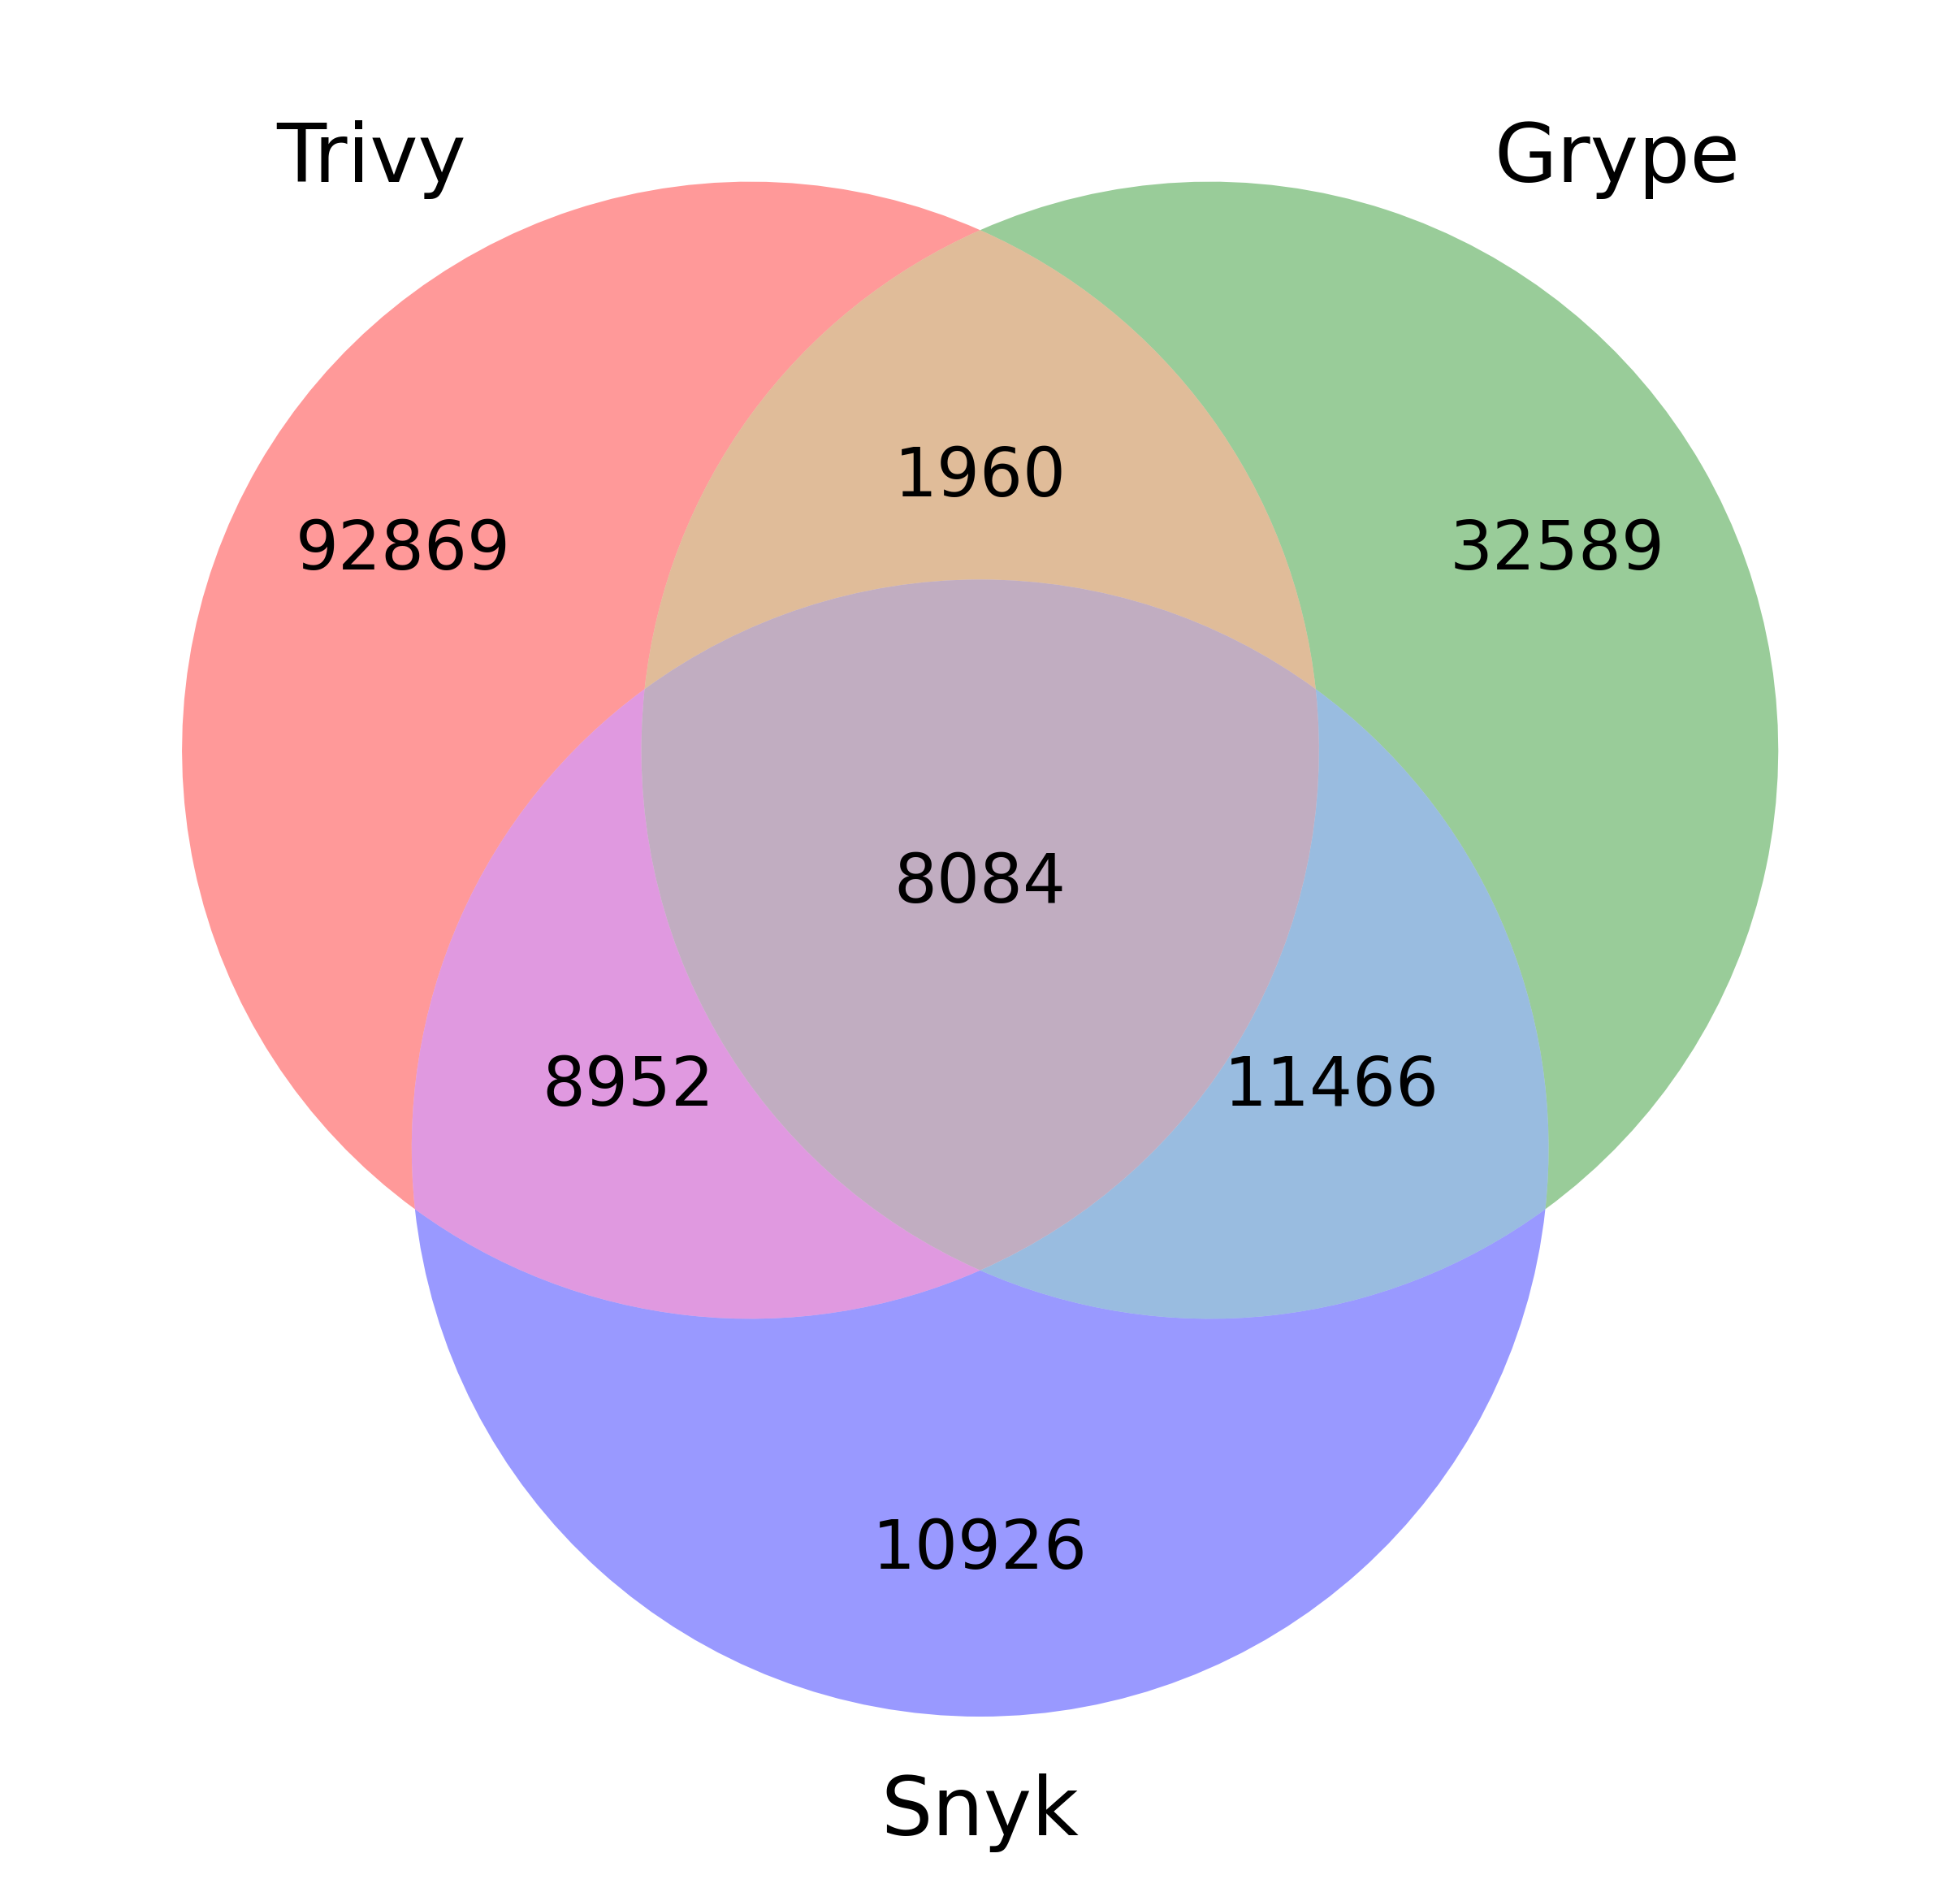
\includegraphics[width=1\linewidth]{images/s1/vulCountsVenn.png}
		\caption{Tüm zafiyetlere ait venn diyagramı.}\label{fig:vulCountsVenn}
	\end{subfigure}

	\caption{Tarama araçları tarafından tespit edilen zafiyet sayısının Venn diyagramı.}\label{fig:fig2}
\end{figure}

Şekil~\ref{fig:vulnerabilities-by-severity} ve tablo~\ref{tab:scanner-vuln-severity}'de güvenlik açığı tespitlerini ciddiyete (severity) göre ayrılmış olarak görebiliriz. Tarama sürecinde, ihmal edilebilir ve bilinmeyen güvenlik açıklarını hariç tutuldu, çünkü ihmal edilebilir güvenlik açıkları ciddi hasara işaret etmez ve bilinmeyen güvenlik açıklarının CVSS puanları yoktur.

\begin{figure}
	\centering
	\begin{subfigure}[Figure A]{\linewidth/2}
		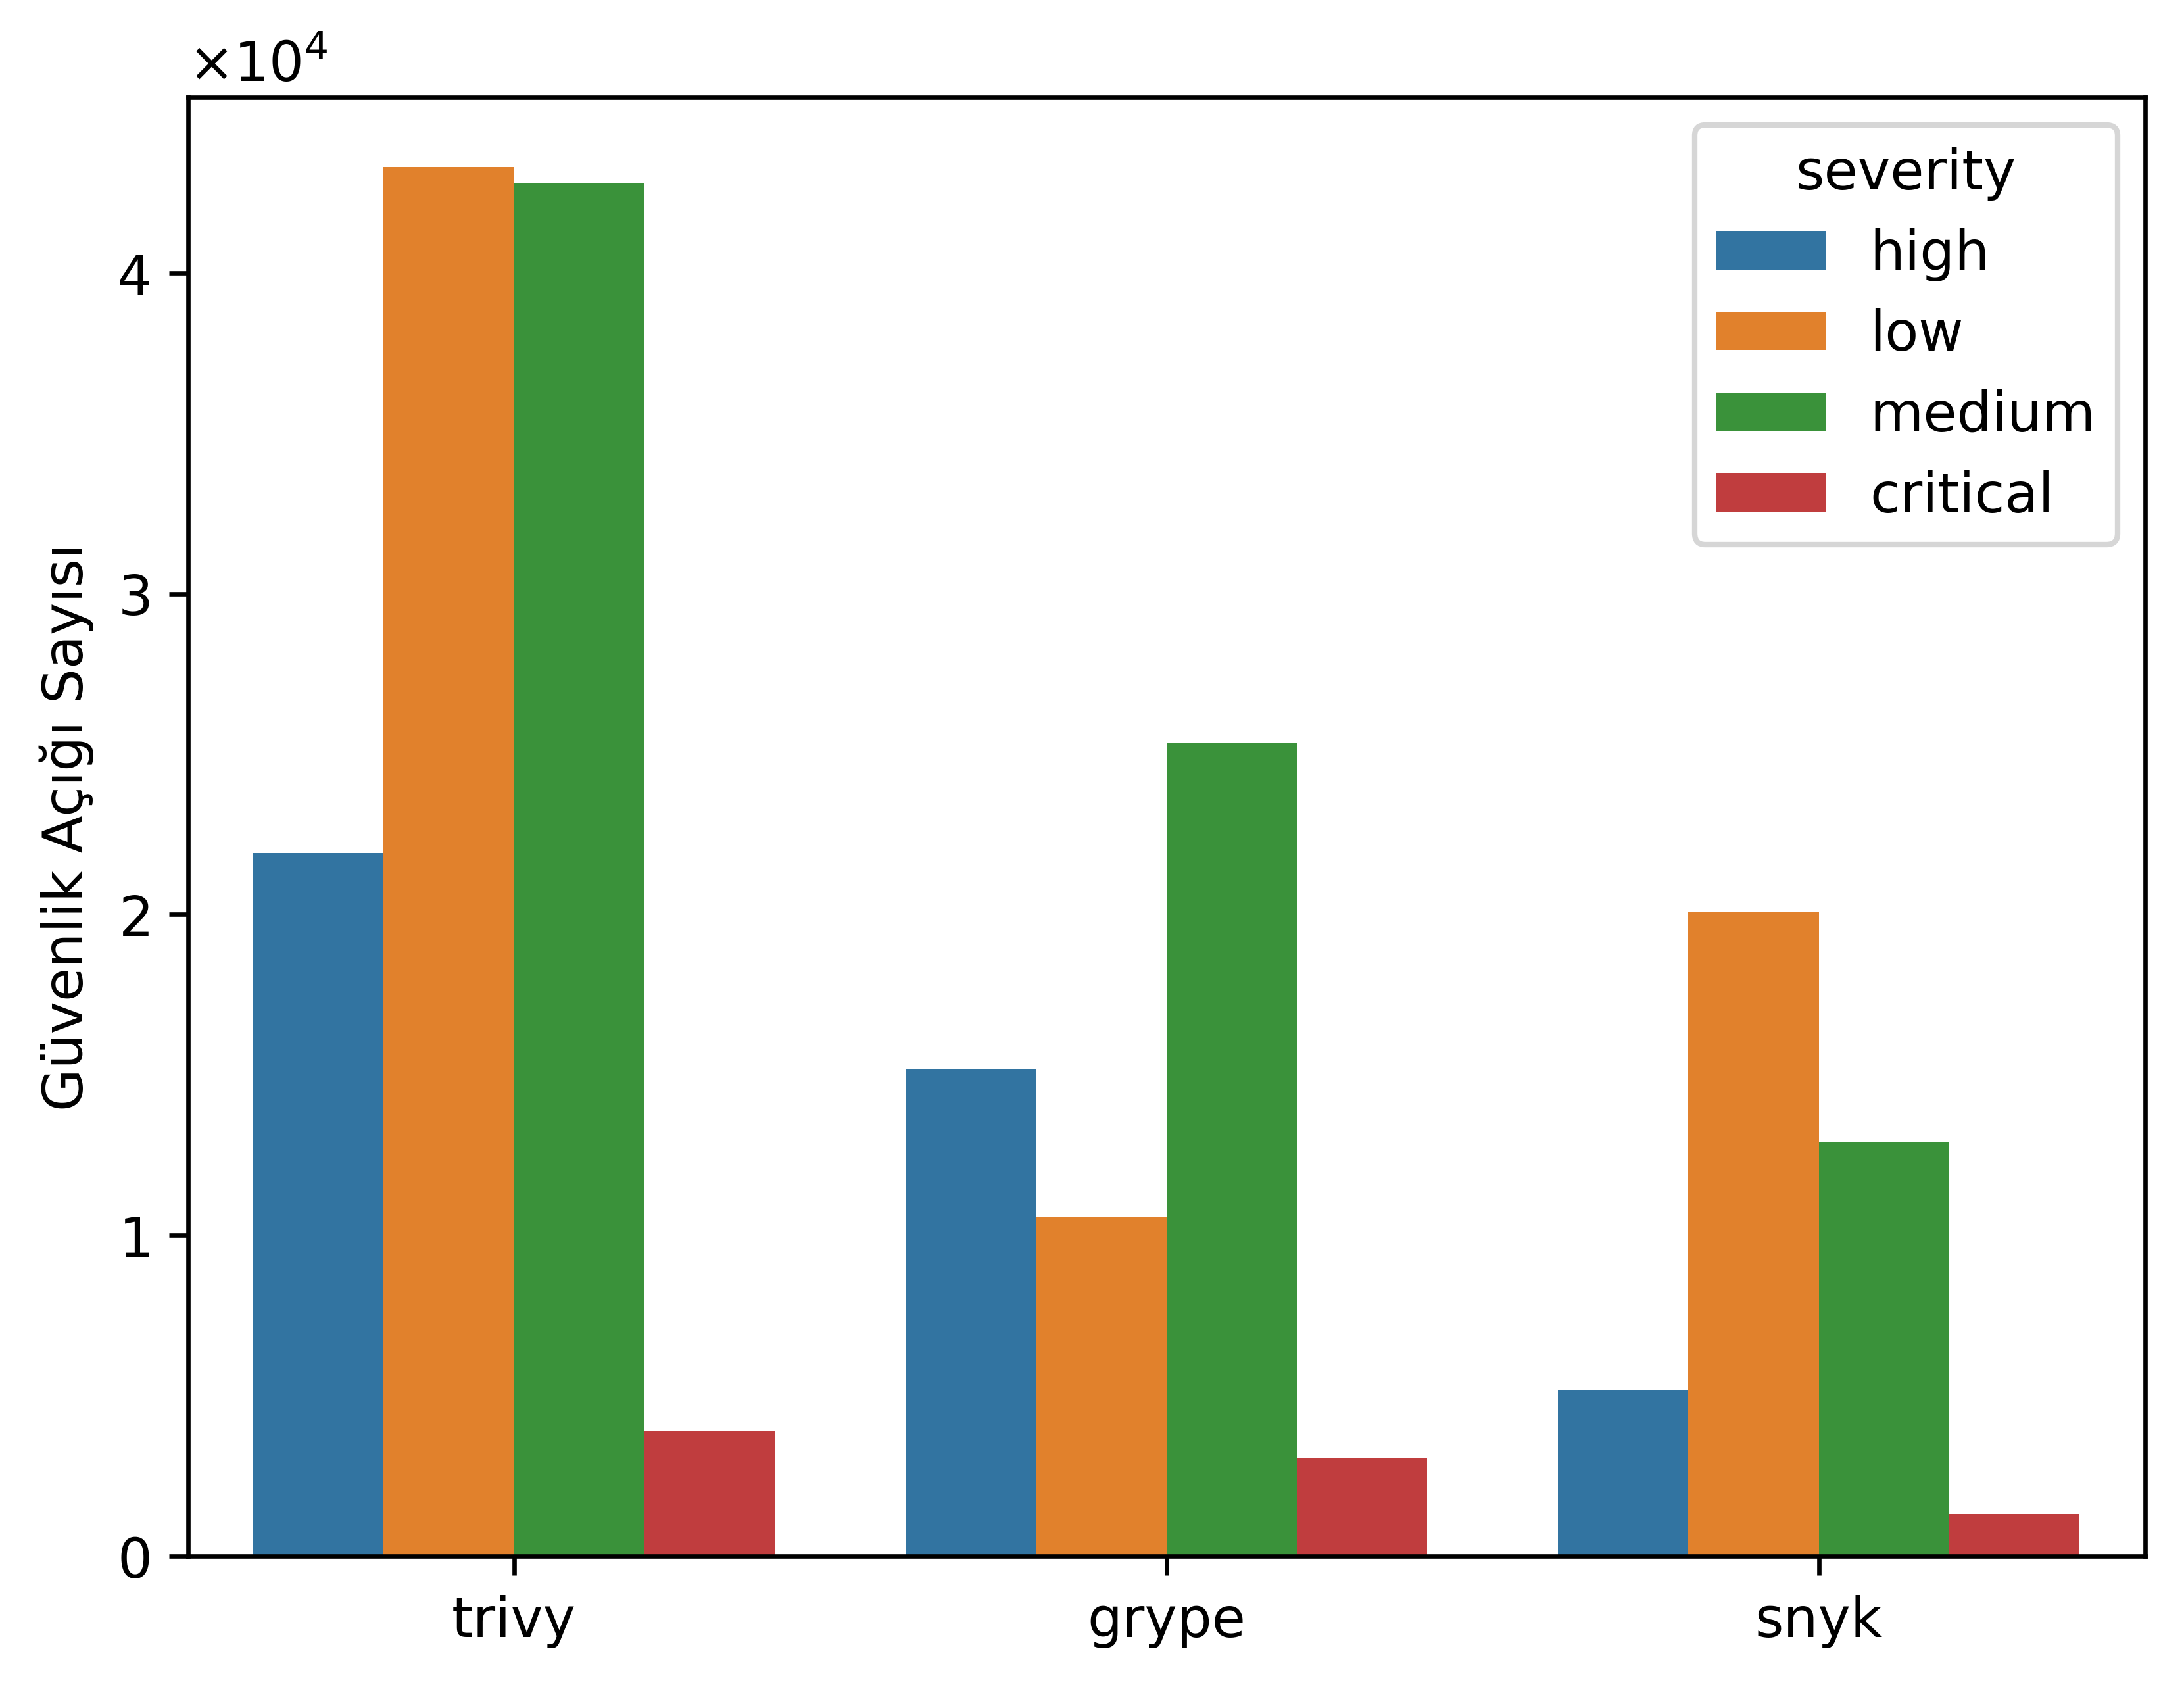
\includegraphics[width=1\linewidth]{images/s1/scanner-vuln-and-severity.png}
		\caption{Tarama aracına göre}\label{fig:vulnerabilities-by-severity}
	\end{subfigure}% vertical
	\begin{subfigure}[Figure A]{\linewidth/2}
		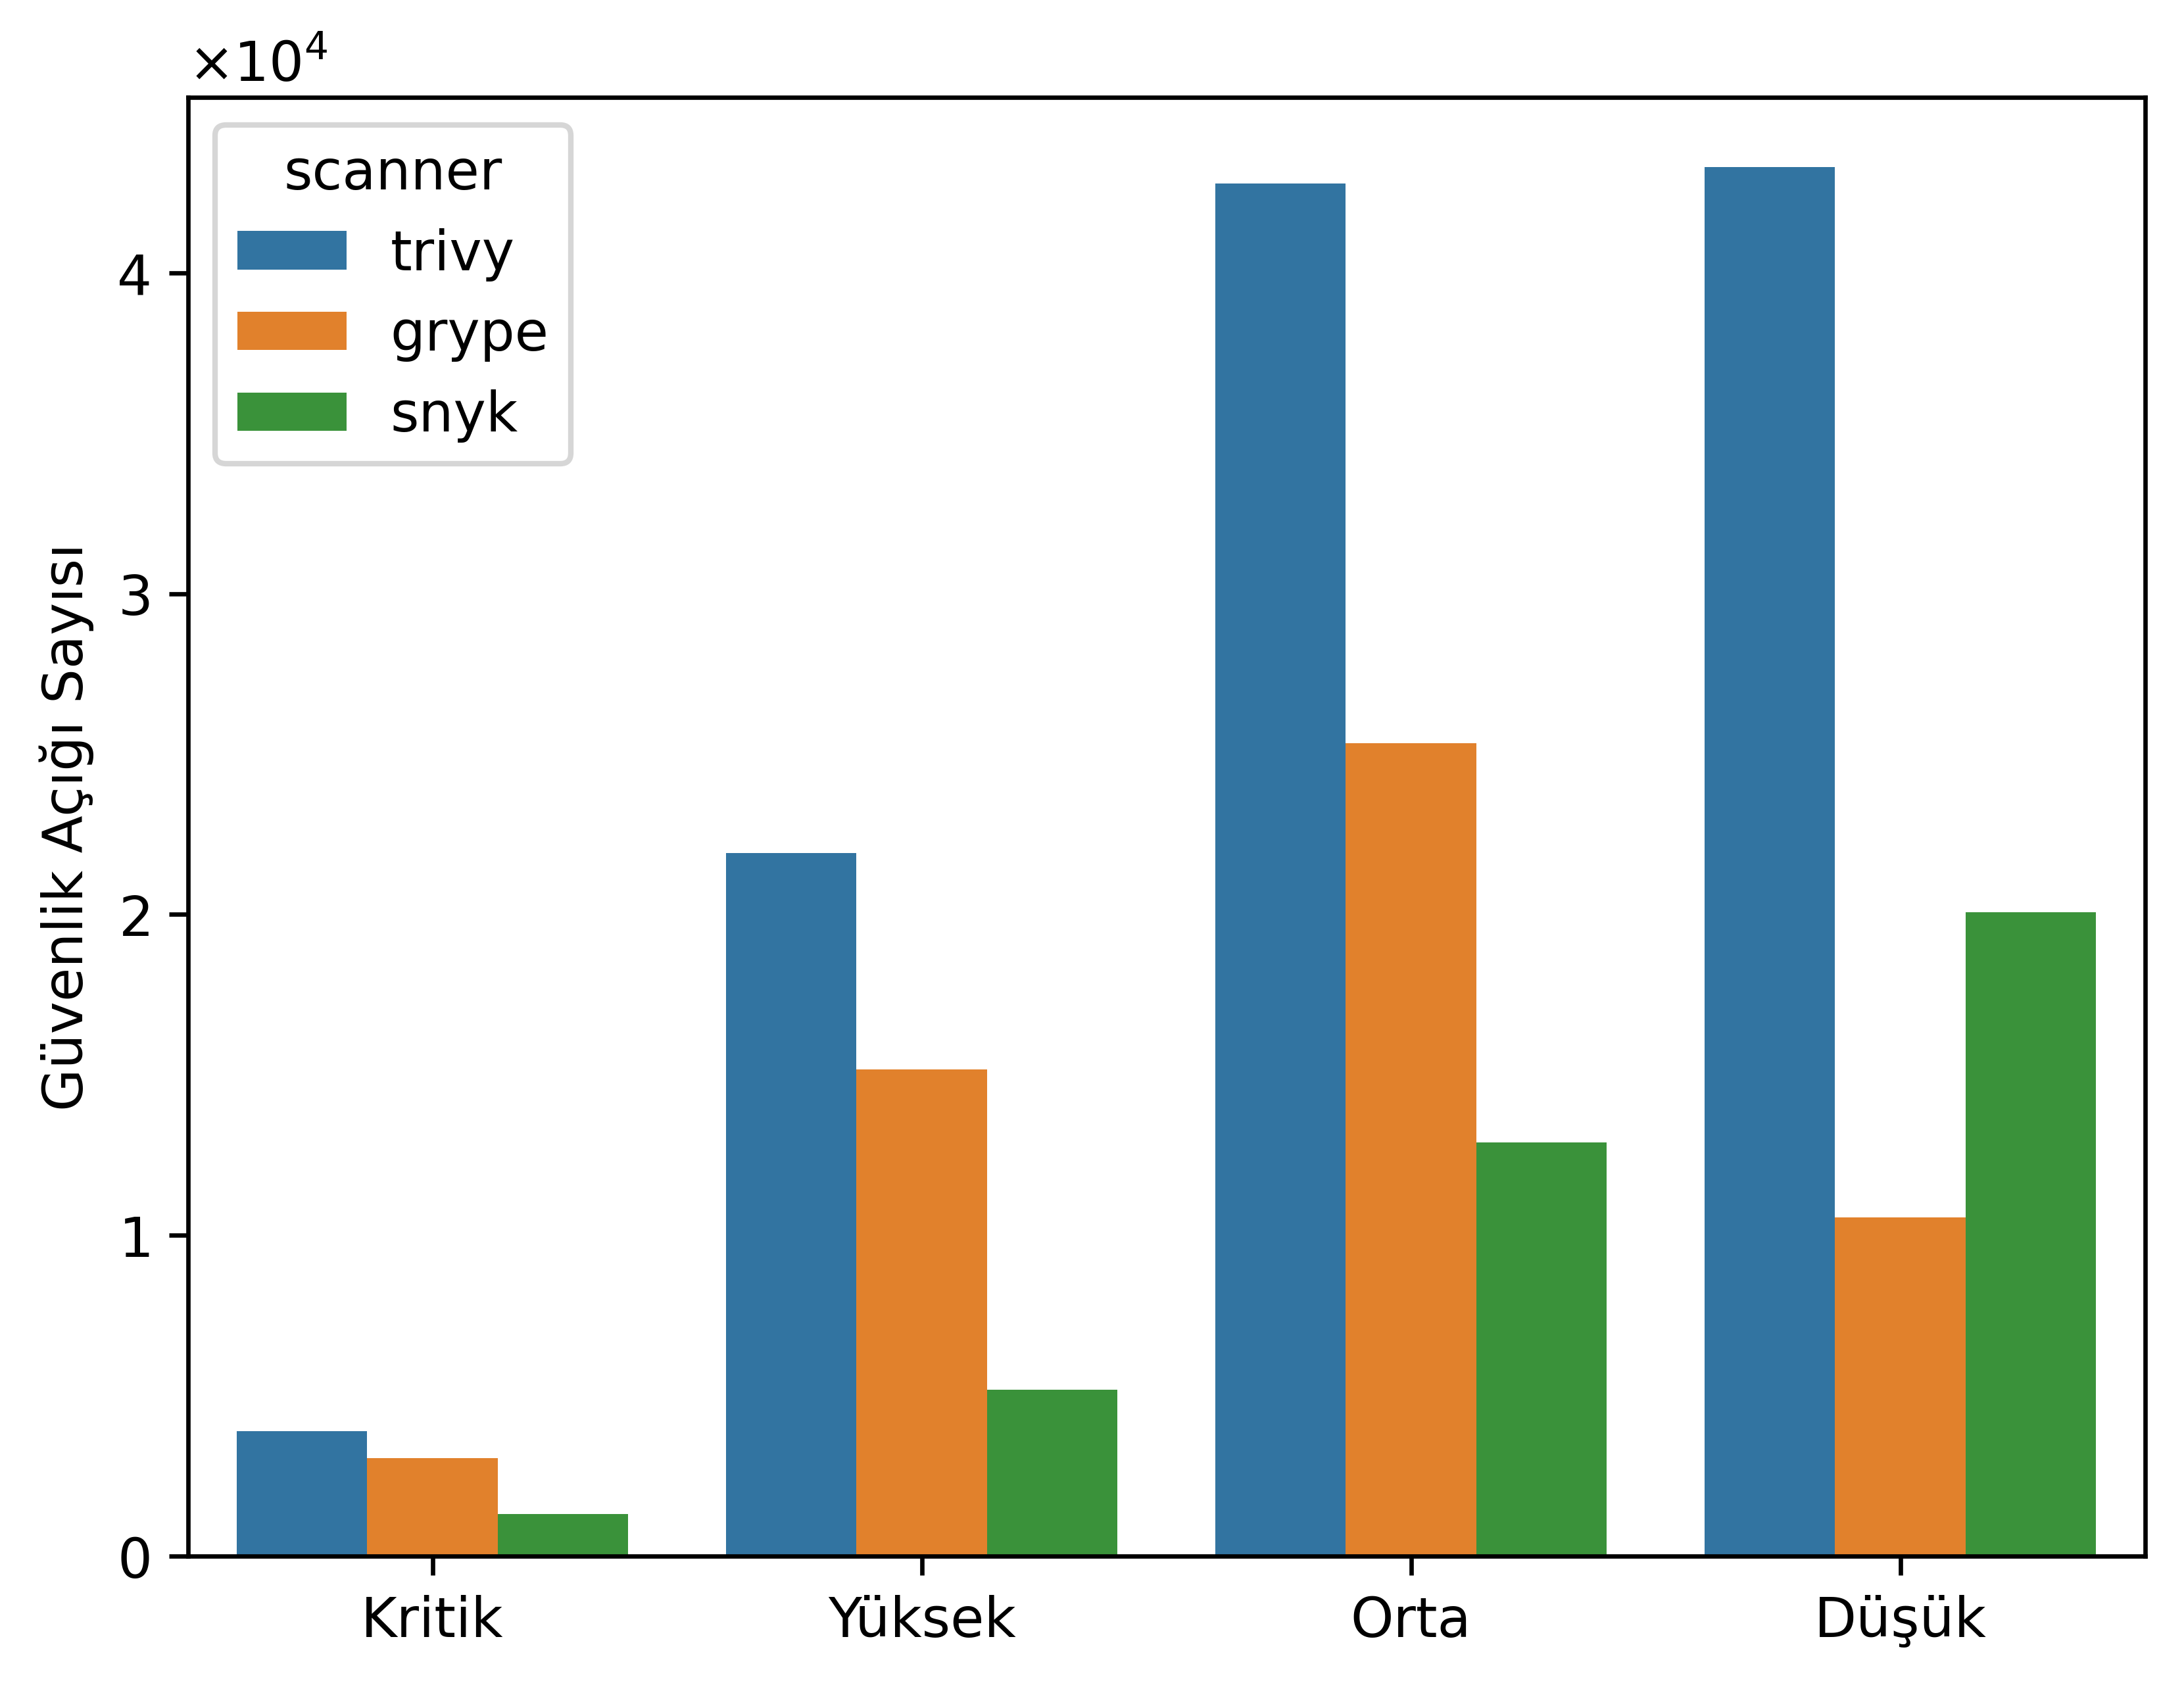
\includegraphics[width=1\linewidth]{images/s1/severity-hue-scanner.png}
    \caption{şiddete göre}\label{fig:severity-hue-scanner}
	\end{subfigure}
 
	\caption{Zafiyetlerin tarama aracına ve şiddete göre dağılımı.}\label{fig:fig3}
\end{figure}

\begin{table}
    \centering
    \begin{tabular}{ |l|c|c|c|c| }
        \hline
        Tarama aracı & Kritik & Yüksek & Orta & Düşük \\
        \hline
        Trivy & 3879 & 21.904 & 42.778 & 43.304 \\
        Grype & 3041 & 15.166 & 25.339 & 10.553 \\
        Snyk  & 1302 & 5184  & 12.880 & 20.064 \\
        \hline
    \end{tabular}
    \caption{Tarayıcı aracına ve önem derecesine göre tespit edilen güvenlik açıkları.}\label{tab:scanner-vuln-severity}
\end{table}

Kritik güvenlik açıkları en tehlikeli ve ciddi güvenlik açıklarıdır. Bu nedenle bu açıkları tespit etmek son derece önemlidir. Şekil~\ref{fig:vulnerabilities-by-severity} ve tablo~\ref{tab:scanner-vuln-severity}'de Trivy'nin 3879 kritik güvenlik açığı tespit ettiğini, Grype'ın 3041 kritik şiddette güvenlik açığı tespit ettiğini ve Snyk'in 1302 tespit ettiğini görebiliriz. Trivy ve ardından Grype kritik güvenlik açıklarını tespit etmede iyi performans göstermektedir. Ancak Snyk, Trivy ve Grype'a kıyasla yeterince iyi performans göstermemiş ve yaklaşık 2000 kritik güvenlik açığını gözden kaçırmıştır.

Yüksek şiddetteki güvenlik açıkları kritik güvenlik açıklarından daha az şiddetlidir ancak yine de tespit edilmeleri önemlidir. Aynı şekilde~\ref{fig:vulnerabilities-by-severity} ve tablo~\ref{tab:scanner-vuln-severity} da Trivy 21.904, Grype 15.166 ve snyk 5184 yüksek şiddette güvenlik açığı tespit etmiştir. Bu istatistiklerden Trivy'nin en iyi performansı gösterdiği ve onu Grype'ın izlediği sonucunu çıkarabiliriz.

Orta şiddette güvenlik açıkları için Trivy 42.778, Grype 25.339 ve Snyk 12.880 güvenlik açığı tespit etmiştir. Düşük önem derecesine sahip güvenlik açıklarında Trivy 43.304, Grype 10.553 ve Snyk 20.064 güvenlik açığı tespit etmiştir.

Genel olarak, Trivy en fazla sayıda güvenlik açığı tespit etmiş, onu kritik, yüksek ve orta önem derecesi kategorilerinde Grype ve Snyk izlemiştir. Ancak, şekil~\ref{fig:fig3}'te gösterildiği gibi, düşük önem dereceli güvenlik açıkları için Trivy en iyi performansı göstermiş, onu Snyk izlemiş ve Grype en düşük tespit oranına sahip olmuştur.

\subsection{İsabet ve Iskalama Metriğine Göre Sonuçlar}\label{subsec:ResultsbyHitandMissMetric}

Bu bölümde, isabet ve ıskalama sonuçlarını hesapladık. İlk olarak, tespit edilen tüm güvenlik açıklarından imaj adı, paket adı, paket sürümü ve CVE ID'sini filtreleyerek eşsiz (unique) güvenlik açıkları tespit ettik. Bu yöntemle toplamda 166.846 benzersiz güvenlik açığı tespit edildi. Daha sonra denklem~\ref{eq:dhr} uygulayarak zafiyet tespit oranları değerlendirildi. Sonuçlar tablo~\ref{tab:hit-and-miss} ve şekil~\ref{fig:hit-and-miss}'de görülebilir.

\begin{table}
    \centering
    \begin{tabular}{ |c|c|c|c| }
        \hline
        Tarama Aracı & Zafiyet Tespit Sayısı & Zafiyet Iska Sayısı & DHR \\
        \hline
        Trivy & 111.865 &  54.981 & 0.67 \\
        Grype &  54.099 & 112.747 & 0.32 \\
        Snyk  &  39.430 & 127.418 & 0.24 \\
        \hline
    \end{tabular}
    \caption{Araçların tespit isabet oranları.}\label{tab:hit-and-miss}
\end{table}

Bu sayılardan ve istatistiklerden, Trivy'nin \%67 isabet oranıyla en iyi performansı gösterdiği sonucunu çıkarabiliriz. Trivy 111.865 adet güvenlik açığı tespit etmiştir, ancak yine de güvenlik açıklarının \%33'ünü kaçırmaktadır; kaçırdığı zafiyetlerin tam sayısı 54.981'dir. Yani en iyi tarama aracı güvenlik açıklarının \%33'ünü kaçırmaktadır. Sonra, Grype 54.099 güvenlik açığı tespit etmiştir ve 112.747 güvenlik açığını kaçırmıştır. Grype'ın DHR'si \%32'dir ve güvenlik açıklarının \%68'ini kaçırmaktadır. Son olarak, Snyk 39.430 güvenlik açığı tespit etmiştir ve \%24 DHR ile 127.418 güvenlik açığını kaçırmıştır. Bu istatistikler şekil~\ref{fig:hit-and-miss}'de görülebilir.

\begin{figure}
    \centering
    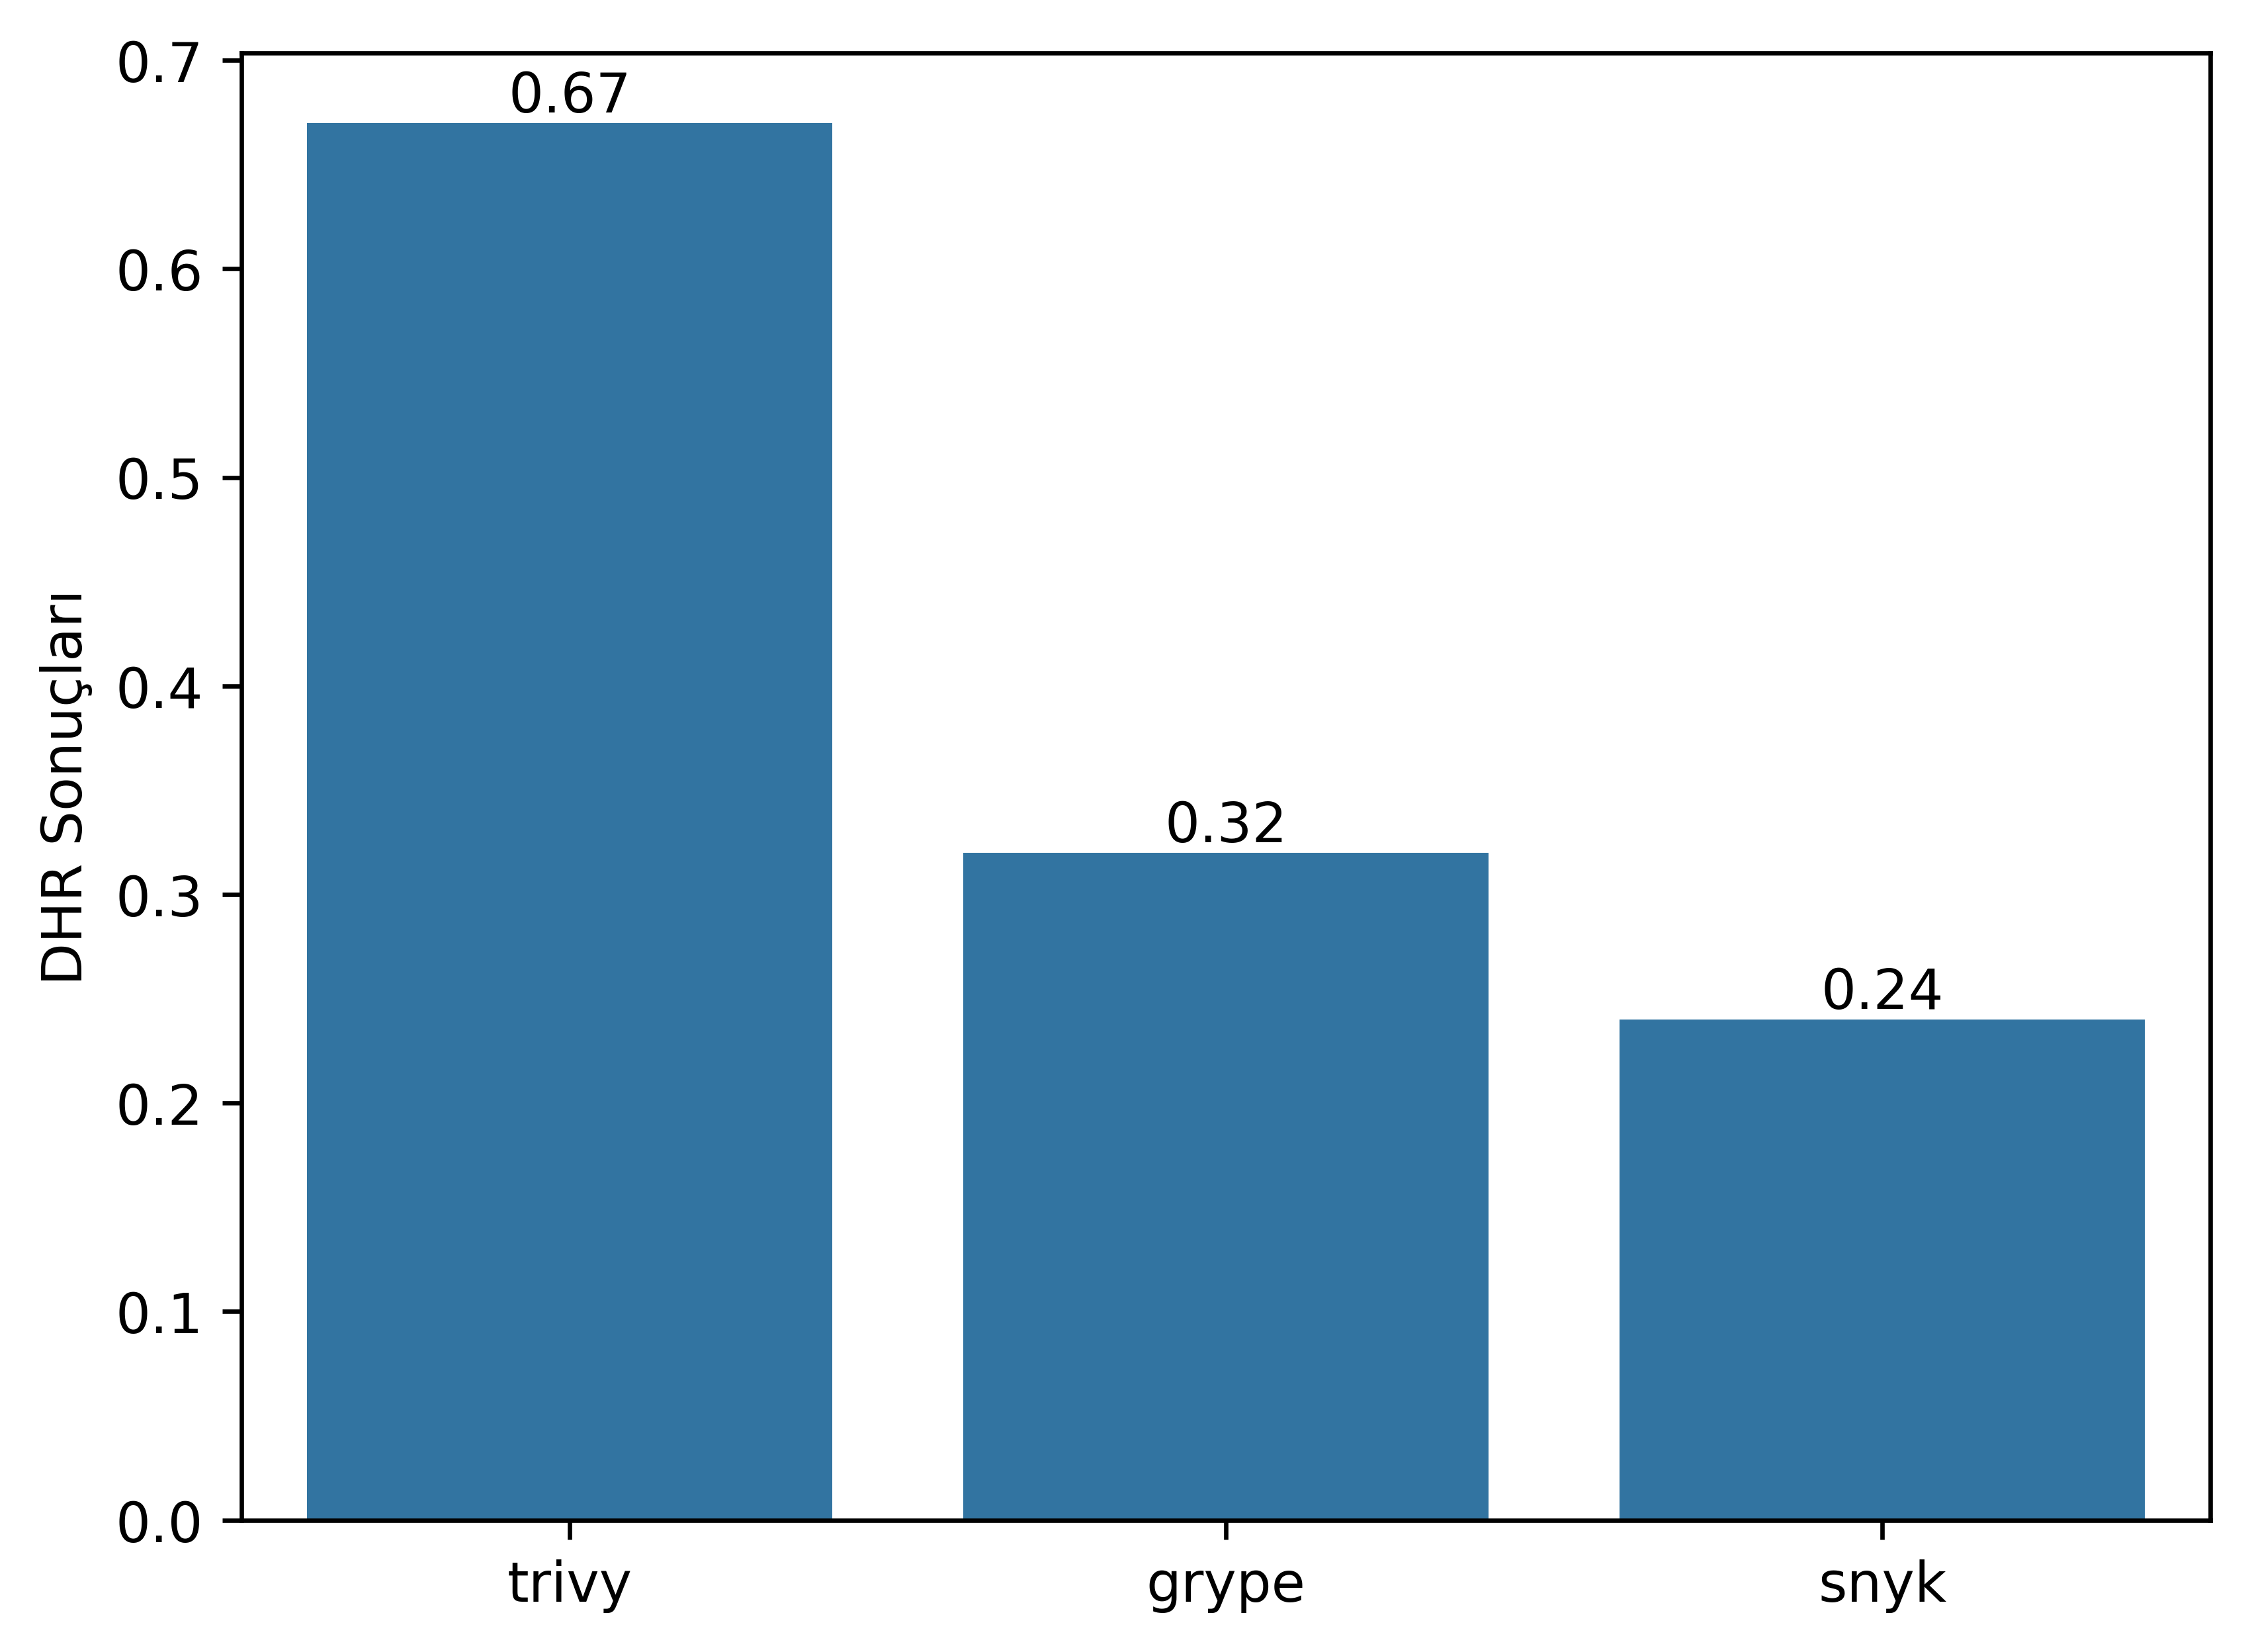
\includegraphics[width=1\linewidth]{images/s1/DHR.png}
    \caption{Tarama araçları zafiyet tespiti oranları.}\label{fig:hit-and-miss}
\end{figure}

\subsection{Zafiyet Puanlama Metriğine (VSM) Göre Sonuçlar}\label{subsec:ResultsbyVulnerabilityScoringMetric}

Tespit İsabet Oranı (DHR) sonuçların değerlendirmesi için önemli bir metrik olarak hizmet vermektedir. Bununla birlikte, güvenlik açıklarının ciddiyeti ve puanı arasında bir ayrım yapmaması ve kritikliklerine bakmaksızın tüm güvenlik açıklarını eşit olarak ele alması, bu metriğin sınırlılığını oluşturmaktadır. Bu soruna yanıt olarak, Güvenlik Açığı Tarama Metriğini (VSM) öneriyoruz. Bu metrik Denklem~\ref{eq:vsm}'de açıklandığı şekilde hesaplanmaktadır. VSM, DHR yöntemine benzer bir yaklaşım izlemektedir. VSM, tüm tarama araçları tarafından bulunan tüm güvenlik açıklarının yer aldığı ortak bir zafiyet havuzu oluşturur. Bir tarama aracının başarısı, bu havuzda bulunan güvenlik açıklarını ne kadar iyi tespit ettiği ile belirlenir. DHR'den farklı olarak VSM yöntemi, tespit edilen güvenlik açıklarının risk seviyelerini dikkate alır. Denklem~\ref{eq:vsm}'de, $n_i$ güvenlik açığının CVSS puanını (bkz. Tablo~\ref{tab:cvss-severity}) temsil eder. Tarama sürecinde, bir güvenlik açığının risk seviyesi için CVSS2 ve CVSS3 olmak üzere iki farklı puan elde edilebilir. Bir güvenlik açığı CVSS3 skorunun mevcut olmadığı durumlarda CVSS2 skoru kullanılır. VSM sonuçları Tablo~\ref{tab:proposed-metric-results} ve Şekil~\ref{fig:proposed-metric-results}'de görülebilir.

VSM yöntemi DHR yöntemi ile benzer bir yaklaşımla çalışmaktadır. Bu metriklerin hesaplanabilmesi için birden fazla tarama aracının kullanılması gerekmektedir. Bütün tarama araçlarının bulduğu güvenlik açıkları ortak bir havuza toplanıp araçların Miss ($M$) değerleri bir aracın havuzda olup da bulamadığı güvenlik açığına göre hesaplanmaktadır. Bu çalışmada tarama araçlarını birbirlerinden bağımsız olarak değerlendirmek için  SVSM metriği önerilmiştir. Bu metrik VSM'de olduğu gibi zafiyetlerin risk seviyelerini göz önünde bulundurmaktadır. VSM'den farklı olarak sadece aracın bulduğu güvenlik zafiyetlerini kullanarak bir sayısal değer üretmektedir. VSM ve SVSM metriklerinde bulunan sayısal değerlerin bire yakın olması tarama aracının daha iyi olduğunu göstermektedir. SVSM sonuçları Tablo~\ref{tab:proposed-metric-results} ve Şekil~\ref{fig:proposed-metric-results}'de görülebilir.

\begin{table}
    \centering
    \begin{tabular}{ |c|c|c|c| }
        \hline
        Tarama Aracı & Zafiyetlerin CVSS Puan Toplamları \\
        \hline
        Trivy & 736.142,5 \\
        Grype & 319.417,0 \\
        Snyk  & 256.872,0 \\
        \hline
    \end{tabular}
    \caption{Bir araç tarafından tespit edilen zafiyet CVSS puanlarının toplamı.}\label{tab:vuln-sum}
\end{table}

Bir sonraki adımda, bölüm~\ref{subsec:ProposedMetric}'deki denklemi uygulayarak güvenlik açığı puanı metriklerini hesapladık. Sonuçlar tablo~\ref{tab:proposed-metric-results} ve şekil~\ref{fig:proposed-metric-results}'de görülebilir.

\begin{table}
    \centering
    \begin{tabular}{ |c|c|c|c| }
        \hline
        Tarama Aracı & DHR & VSM & SVSM \\
        \hline
        Trivy & 0.67 & 0.44 & 0.44 \\
        Grype & 0.32 & 0.22 & 0.28 \\
        Snyk  & 0.24 & 0.16 & 0.22 \\
        \hline
    \end{tabular}
    \caption{Önerilen metrik ve DHR ile hesaplanan sonuçlar.}\label{tab:proposed-metric-results}
\end{table}

Bu rakamlar, Trivy'nin \%44 oranla en iyi performansı gösterdiğini, Grype'ın \%22 oranla ikinci sırada yer aldığını ve Snyk'in \%16 oranla üçüncü sırada olduğunu açıkça göstermektedir.

% \begin{figure}
%     \centering
%     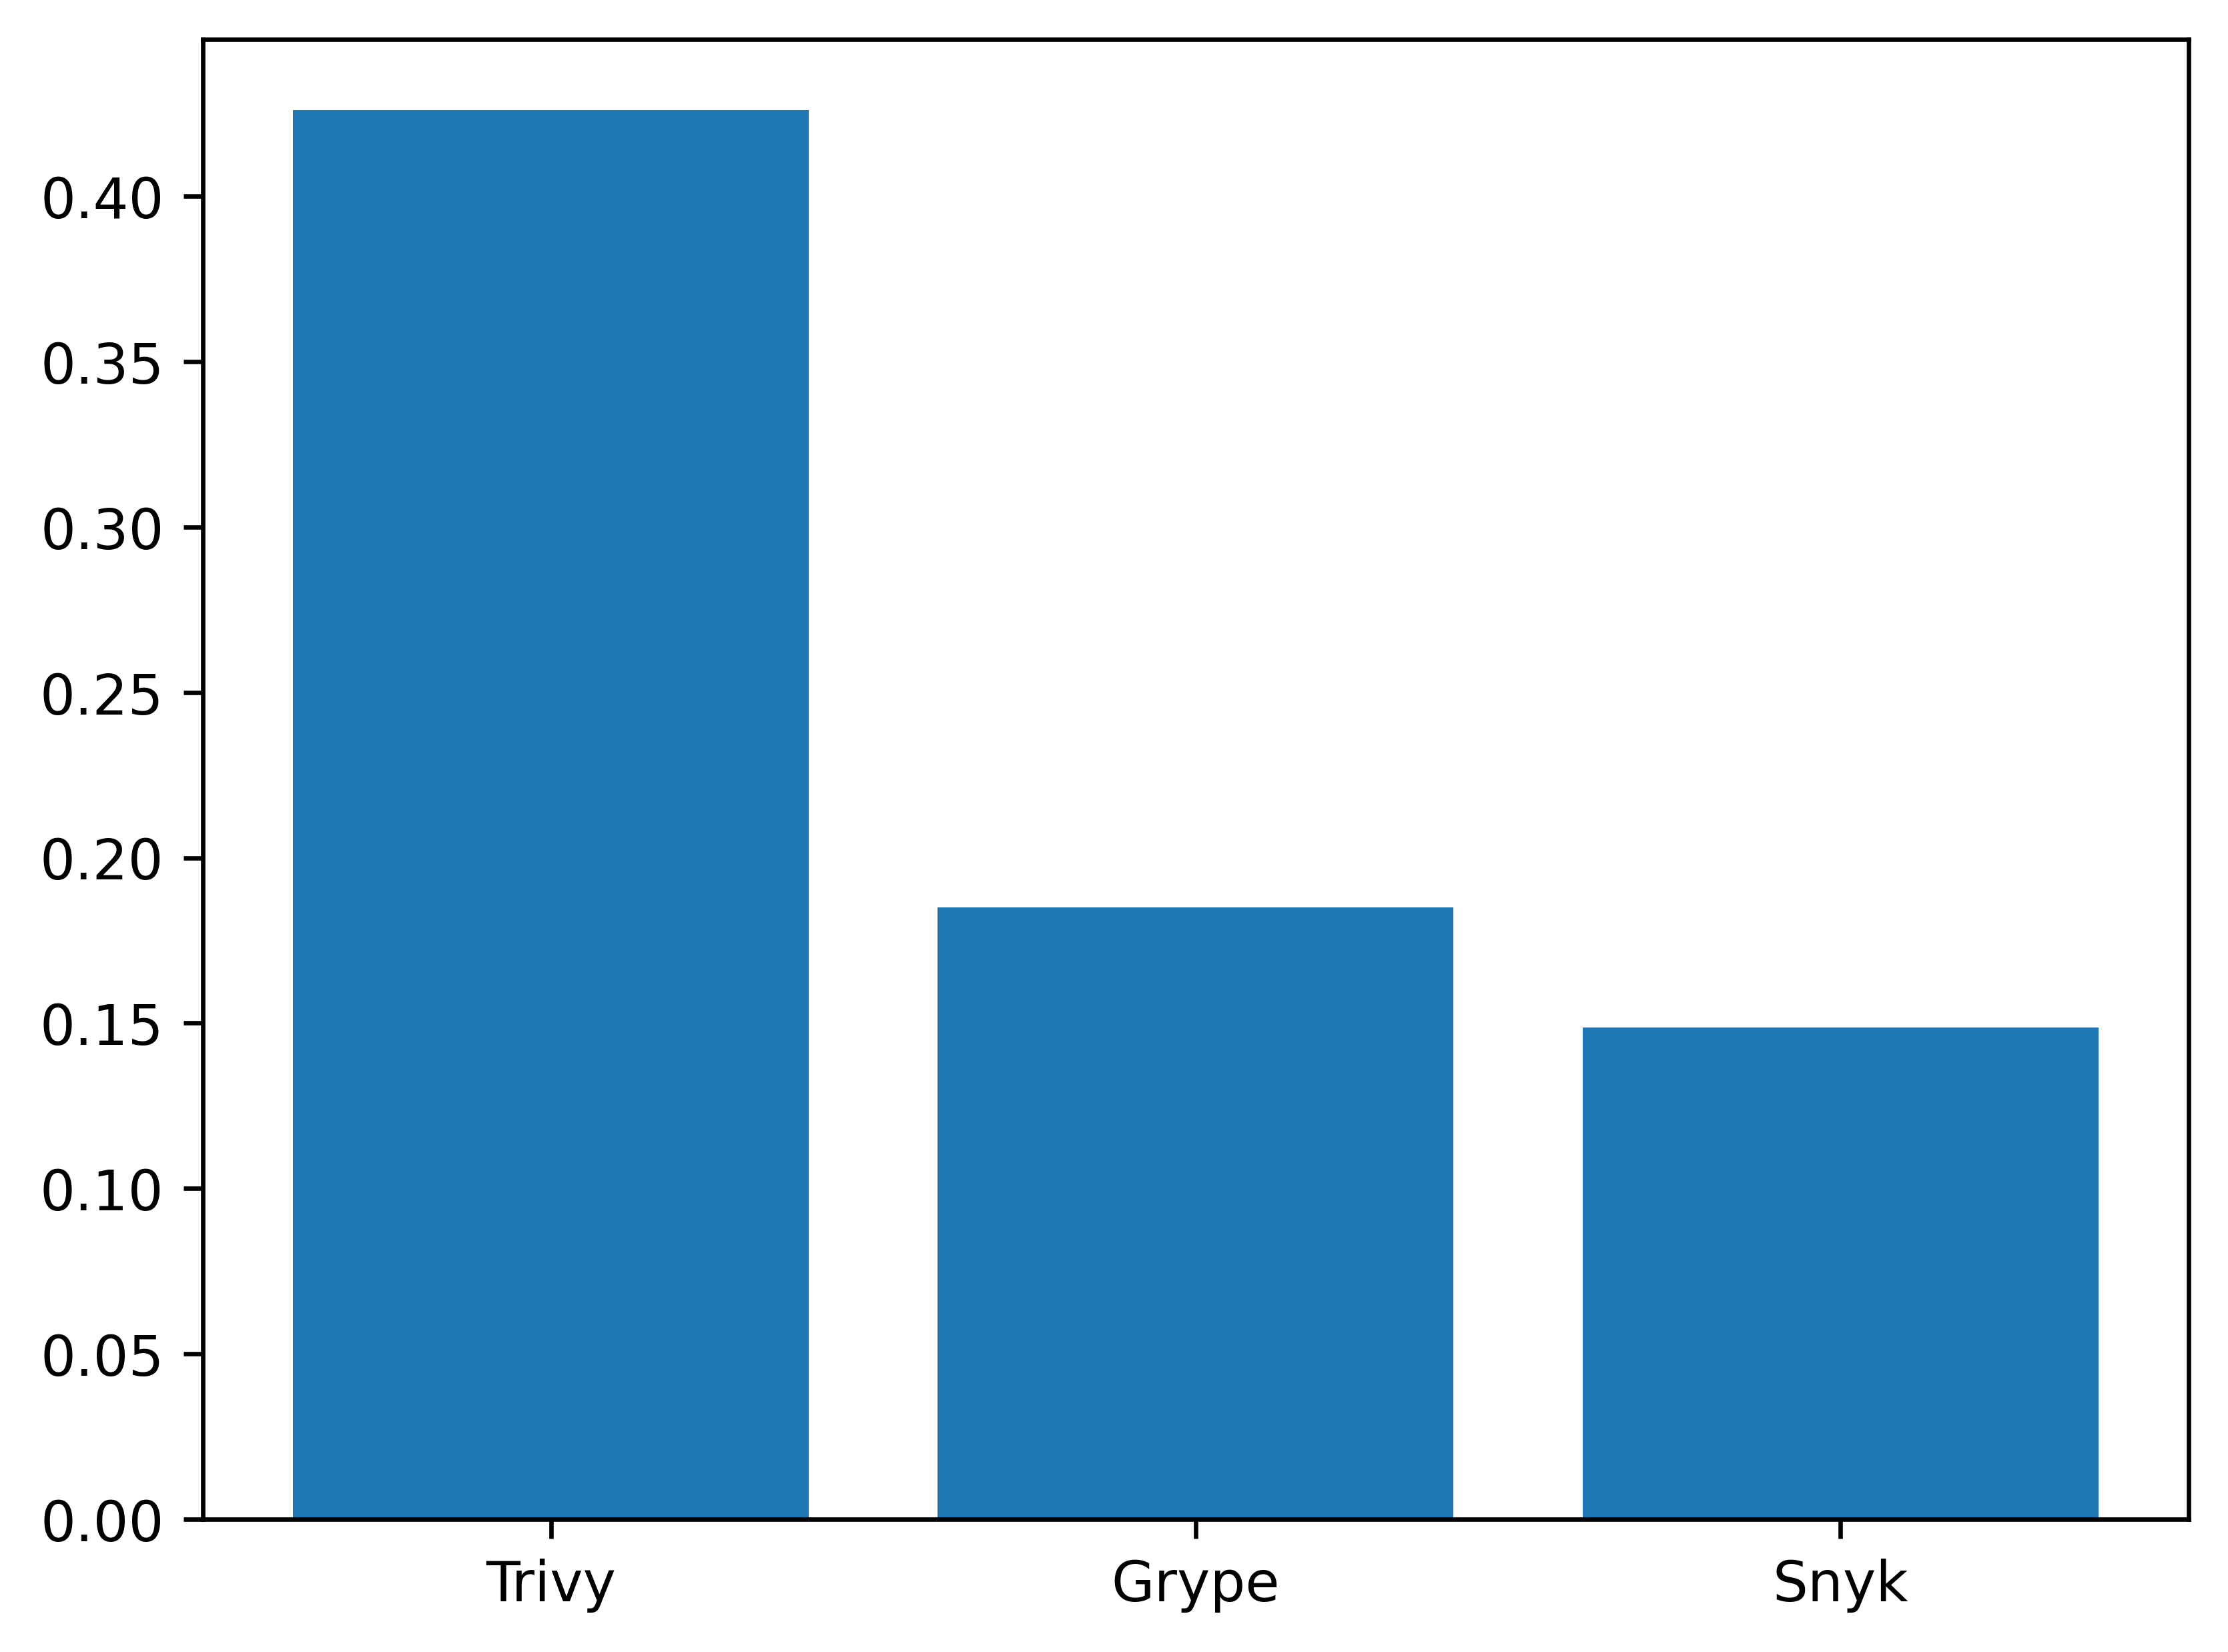
\includegraphics[width=1\linewidth]{images/proposed-metric-results.png}
%     \caption{Önerilen metrik ile hesaplanan sonuçlar}\label{fig:proposed-metric-results}
% \end{figure}

\begin{figure}
	\centering
	\begin{subfigure}[]{\linewidth/2}
		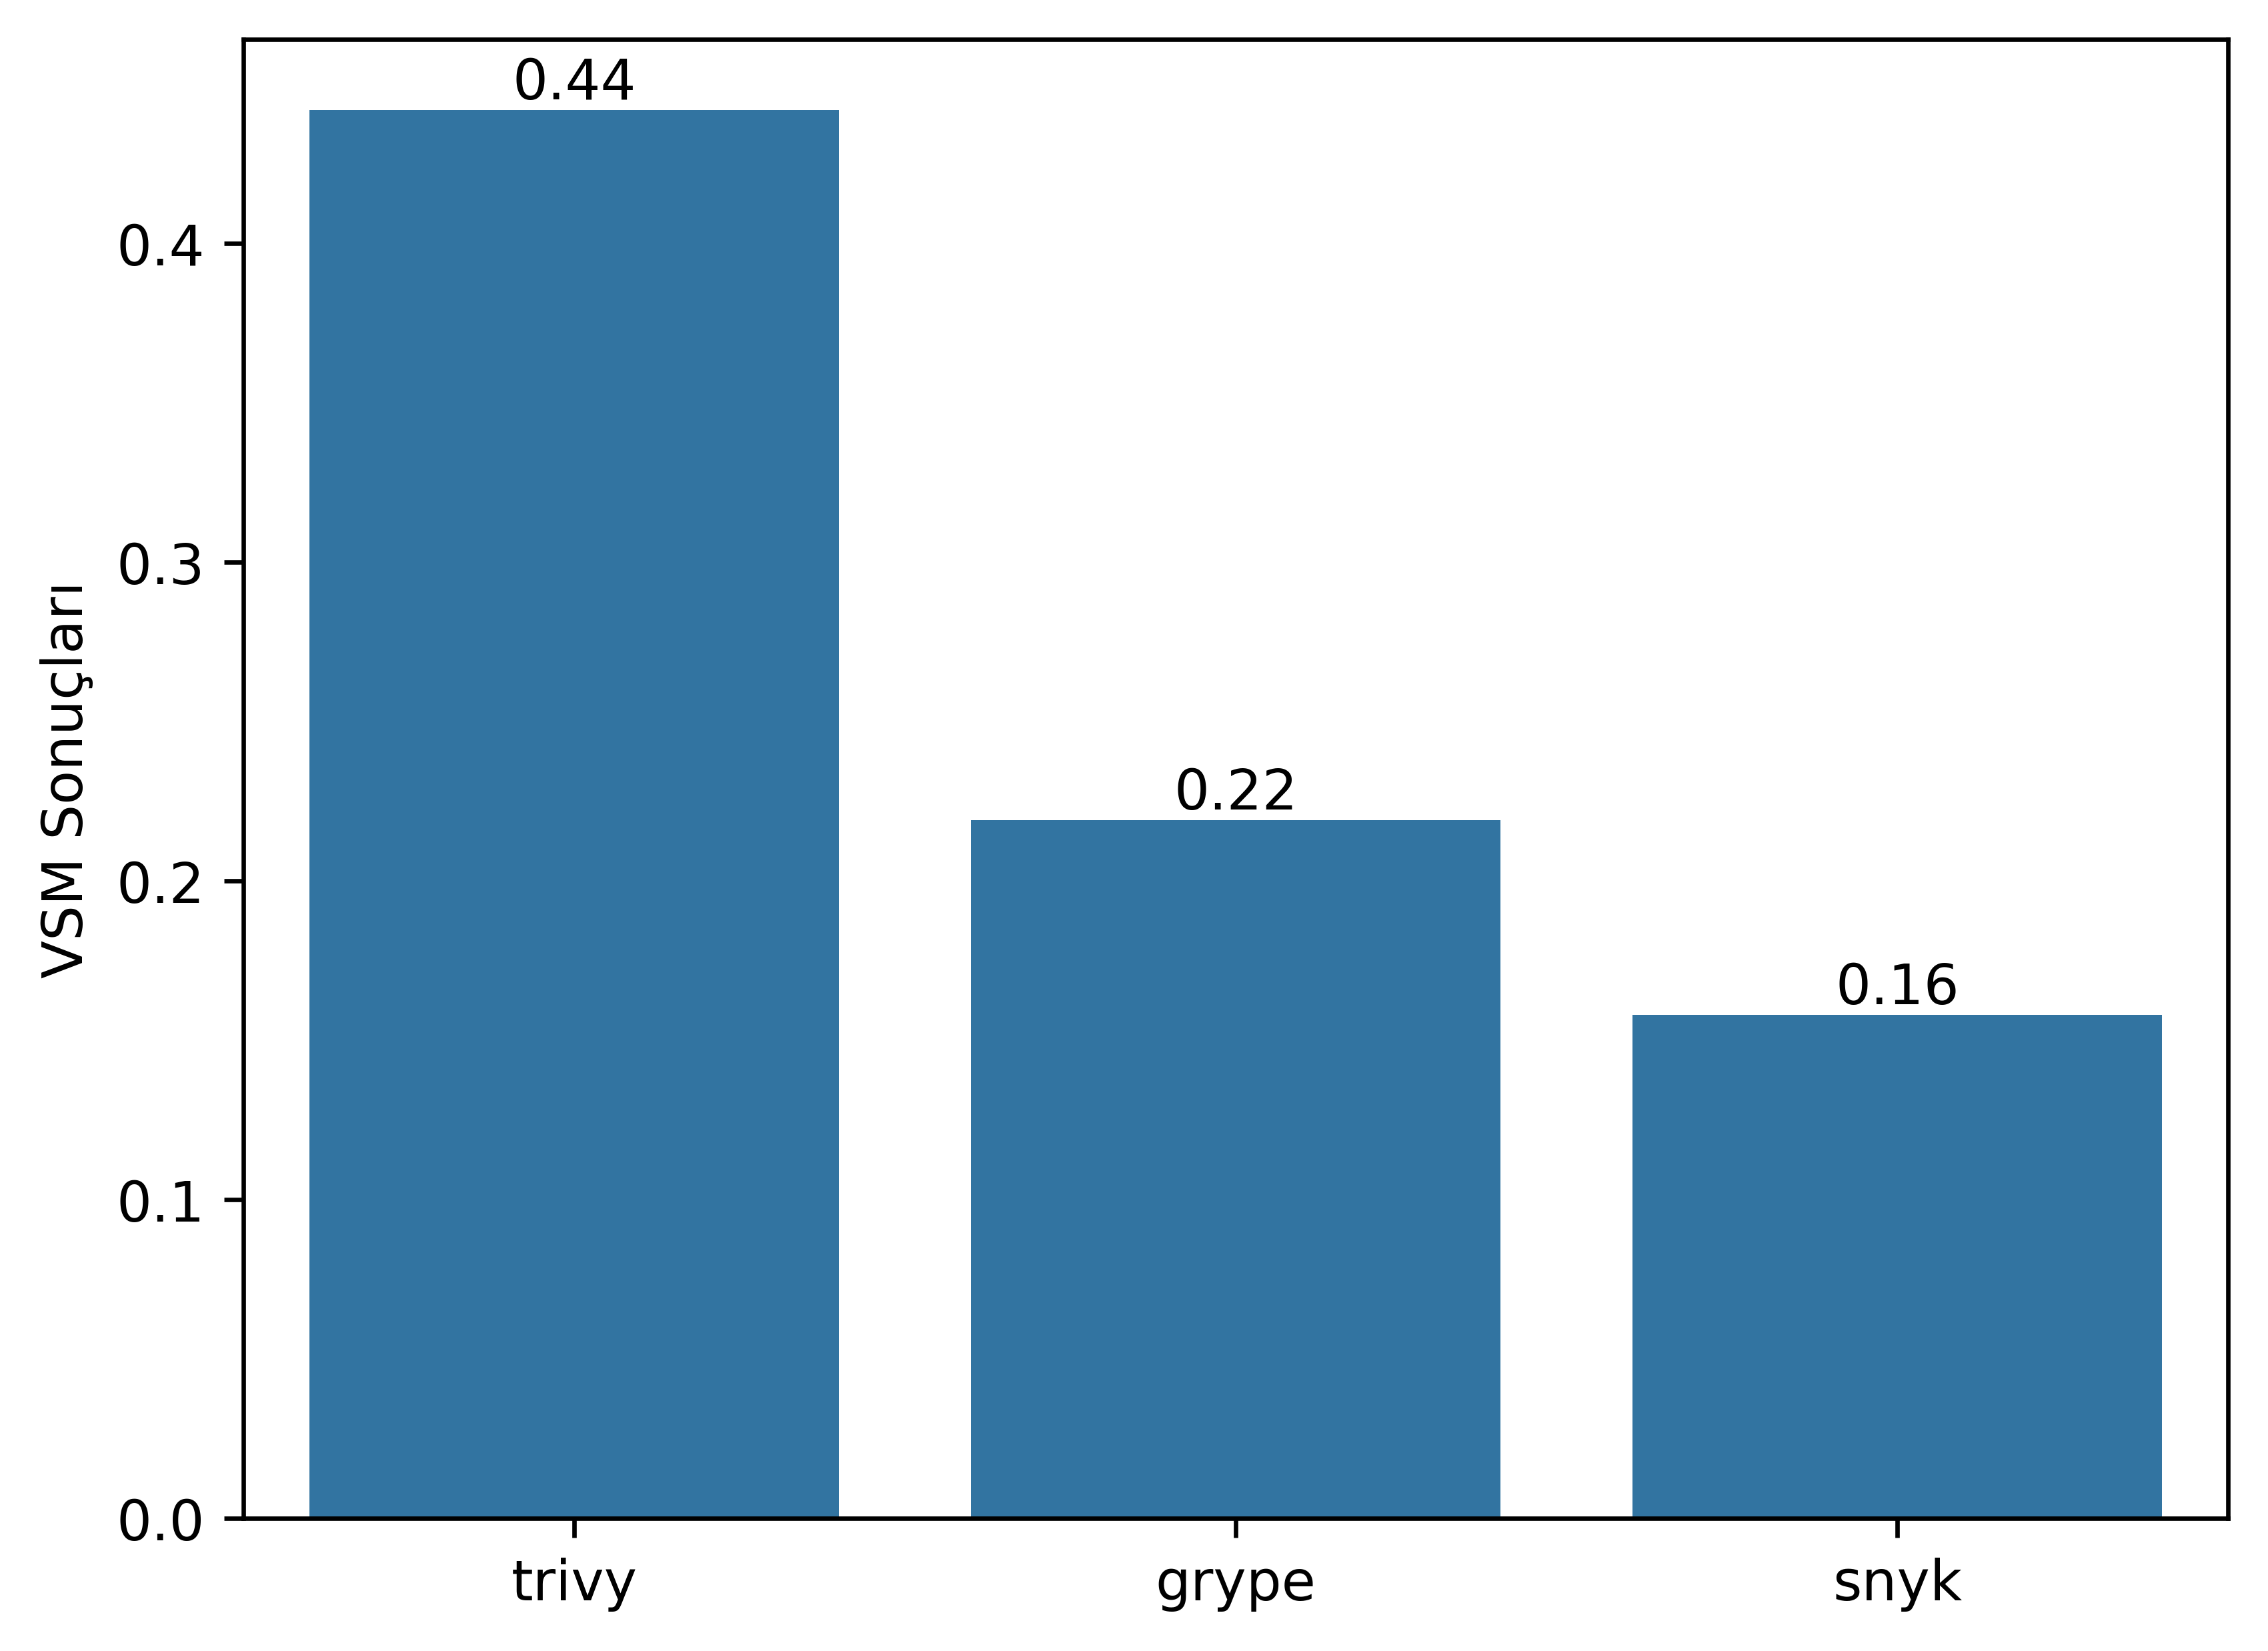
\includegraphics[width=\linewidth]{images/s1/VSM.png}
		\caption{VSM ile hesaplanan sonuçlar}\label{fig:vsm}
	\end{subfigure}%
	\begin{subfigure}[]{\linewidth/2}
		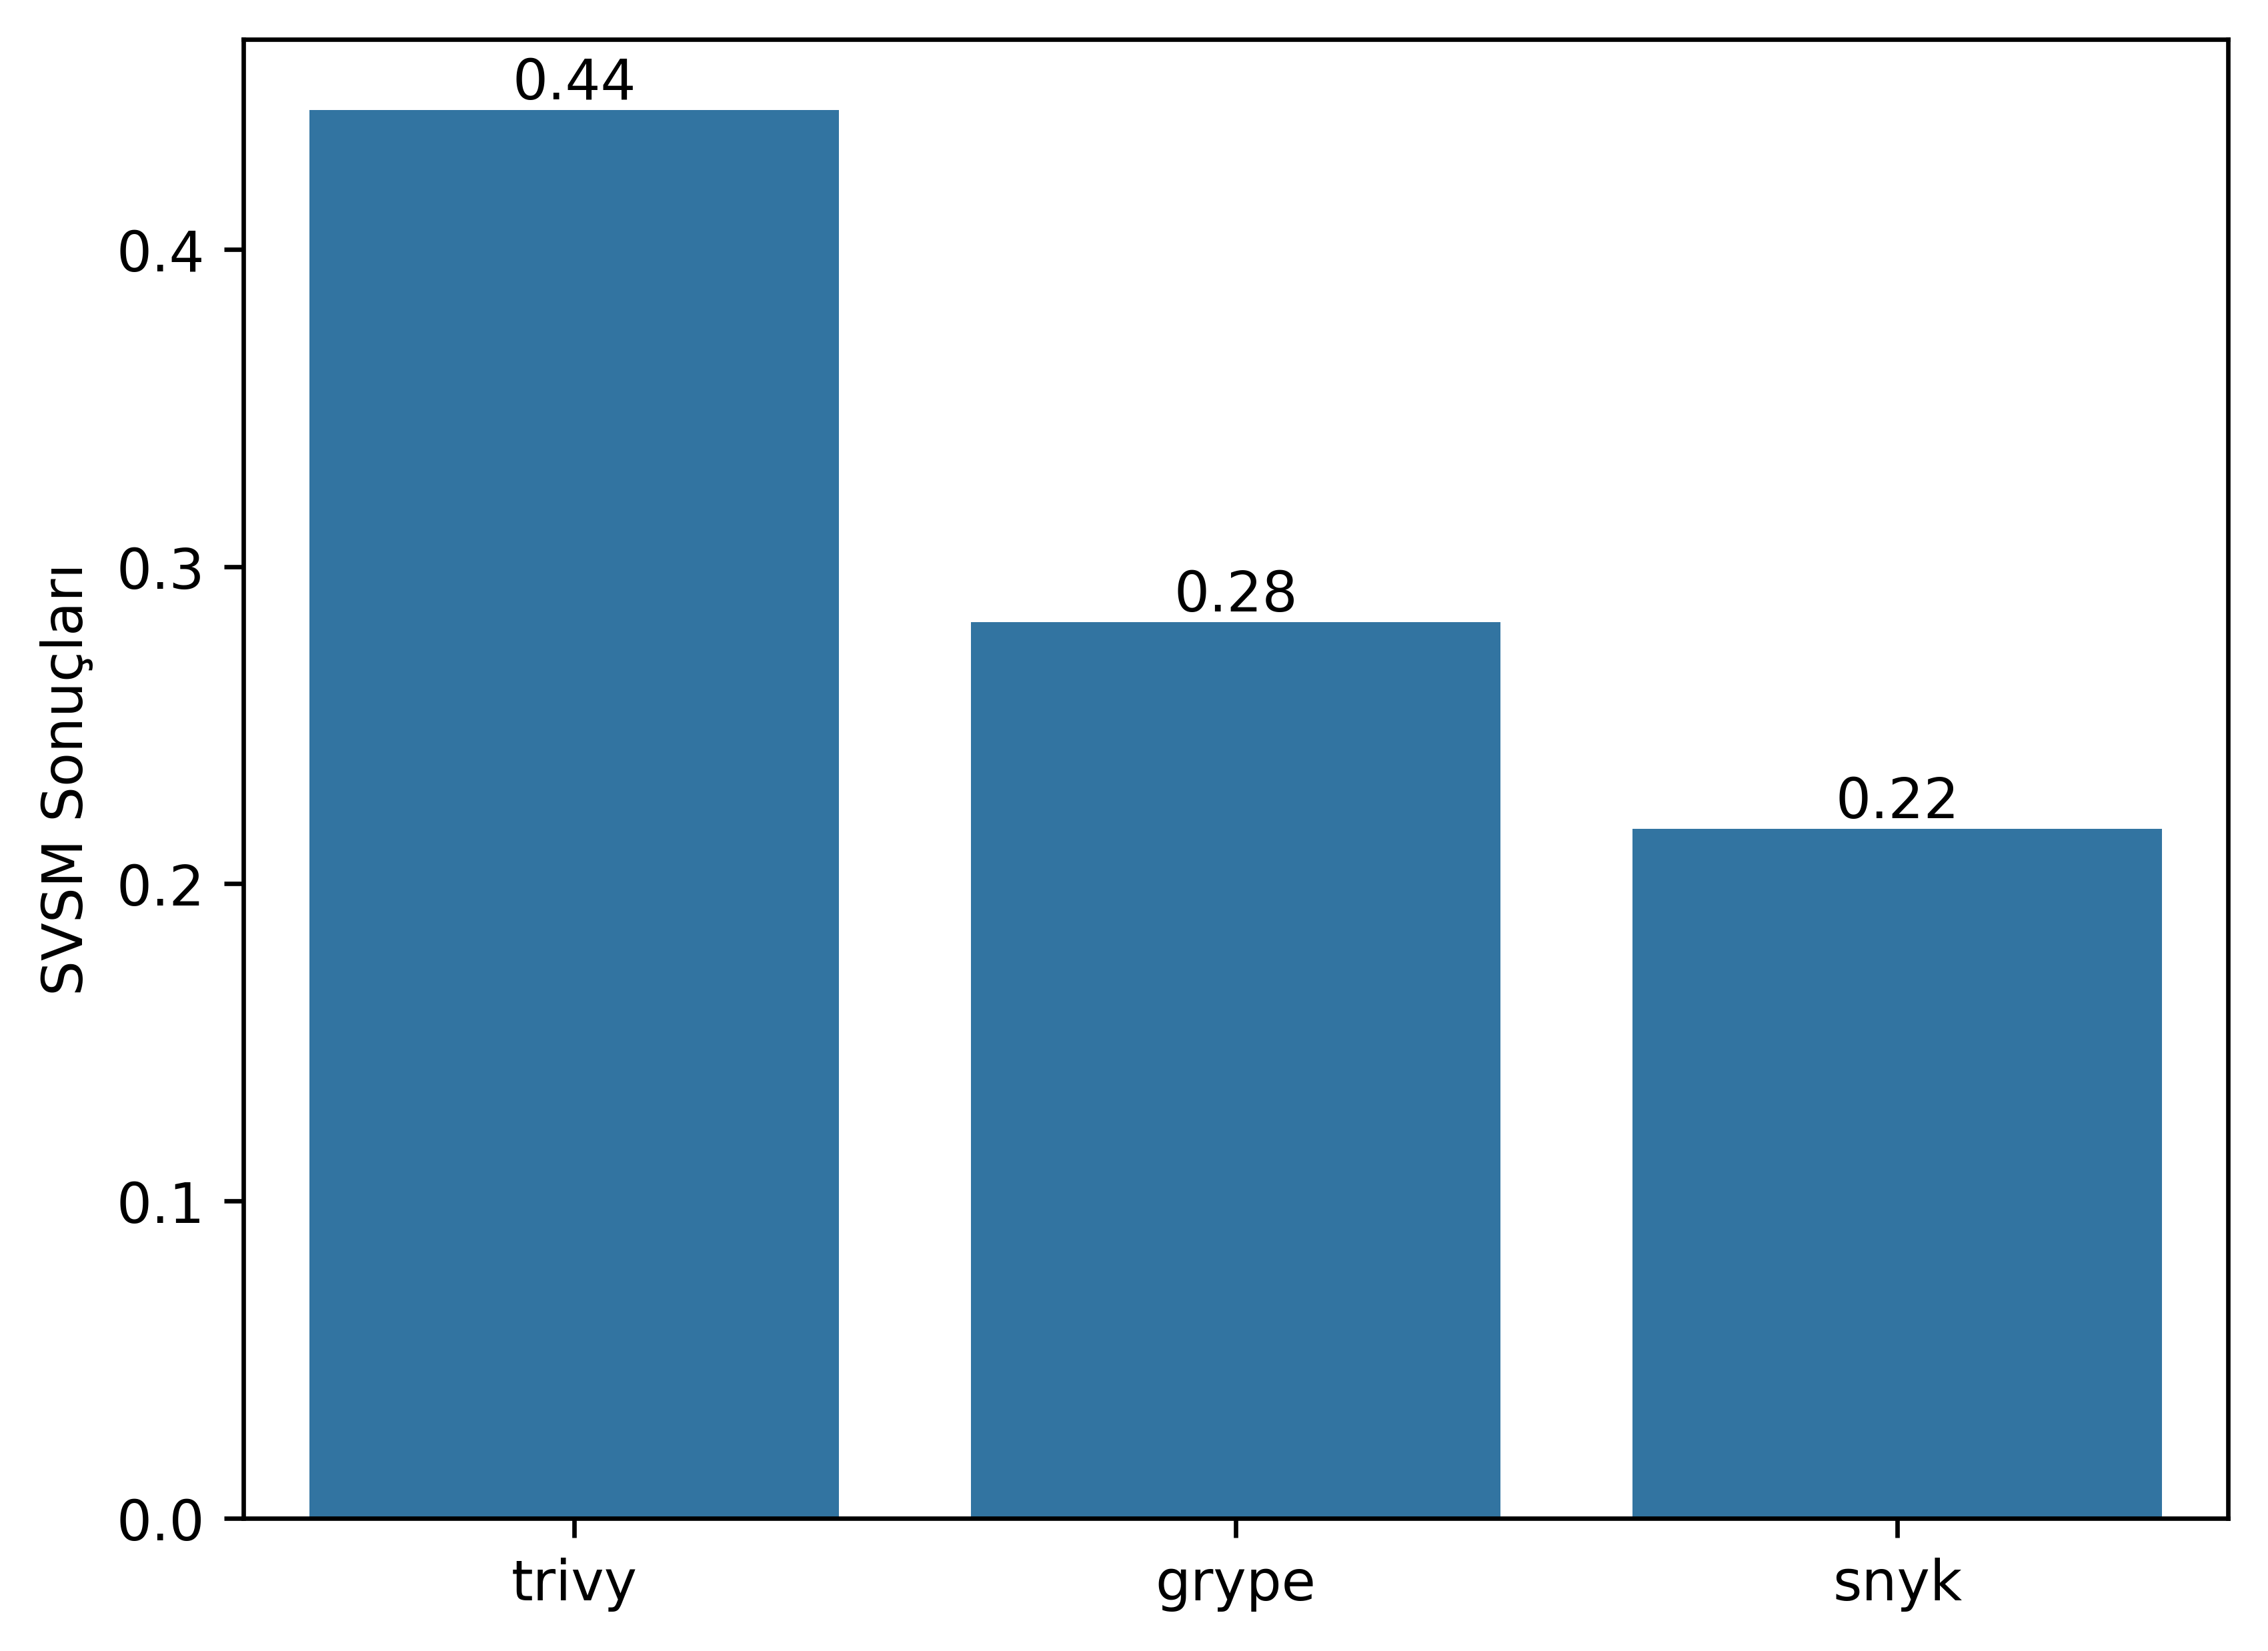
\includegraphics[width=\linewidth]{images/s1/SVSM.png}
		\caption{SVSM ile hesaplanan sonuçlar}\label{fig:svms}
	\end{subfigure}

	\caption{Önerilen metrik ile hesaplanan sonuçlar.}\label{fig:proposed-metric-results}
\end{figure}

\subsection{Metrikler Arası Karşılaştırma}\label{subsec:ComparisonBetweenMetrics}

Önceki bölümlerde sonuçlar 2 farklı metrik ile analiz edildi. Bu bölümde metrik sonuçları karşılaştırılmıştır. Başlangıçta sonuçlar aynı görünüyor ancak bazı önemli farklılıklar mevcut.

İlk olarak VSR'miz DHR'den daha az oran göstermektedir. Bunun nedeni DHR'nin yalnızca tespit edilen güvenlik açığı sayısına dayanması, ancak bizim metriğimizde ortaya çıkan oranın güvenlik açığının CVSS puanlarına dayanmasıdır. Örneğin tablo~\ref{tab:scanner-vuln-severity}'de Trivy'nin 3879 kritik, 21.904 yüksek, 42.778 orta ve 43.304 düşük şiddette güvenlik açığı tespit ettiği görülebilir. Bu önem dereceleri DHR için önemli değildir, ancak VSR için bu önem derecesi farkı sonuç oranını düşürür çünkü tarama araçları daha az kritik güvenlik açıkları tespit eder. Sonuç grafiğini şekil~\ref{fig:comparison-dhr-vsr}'da görebiliriz.

\begin{figure}
    \centering
    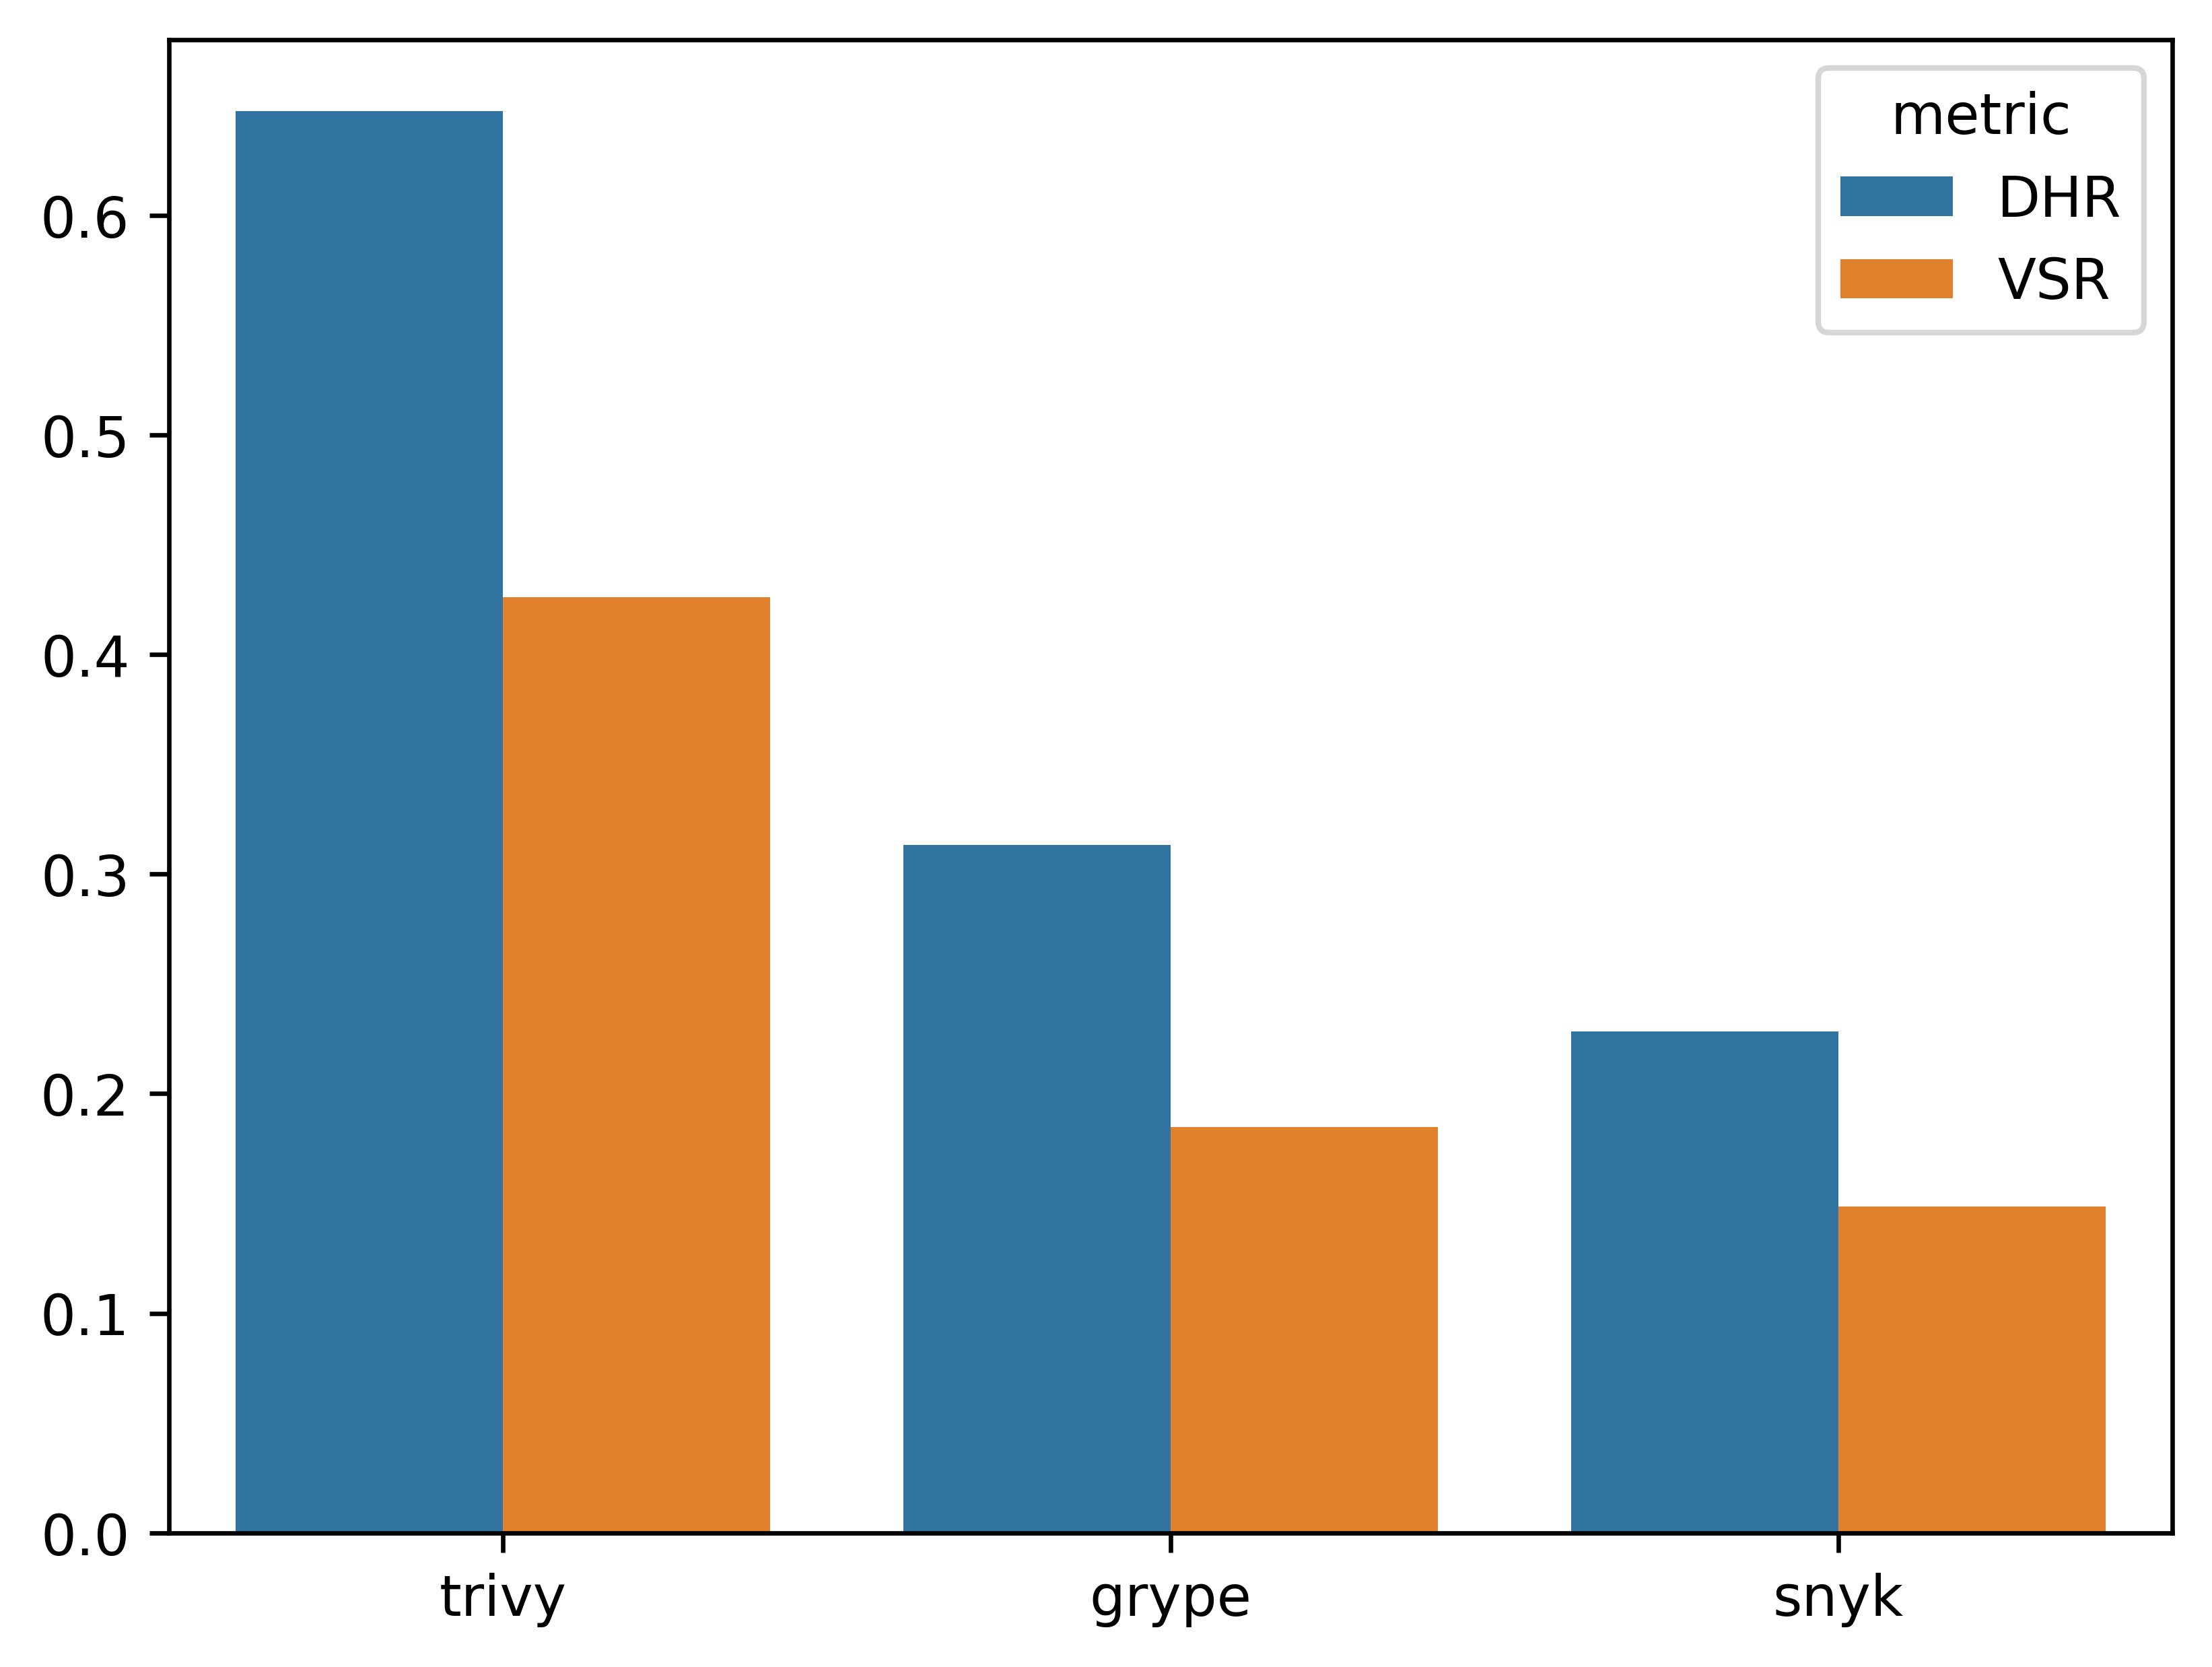
\includegraphics[width=1\linewidth]{images/s1/comparison-dhr-vsr.png}
    \caption{DHR ve VSR'nin Karşılaştırılması}\label{fig:comparison-dhr-vsr}
\end{figure}

\chapter{Araştırma 2}\label{ch:arastirma2}

Her gün yeni güvenlik açıkları keşfedilmekte ve bu açıkları düzeltmek için güvenlik güncellemeleri yayınlanmaktadır. Dolayısıyla bir Docker imajının zaman içerisindeki güvenlik zafiyet durumu farklı olmaktadır. Tezin bu bölümde Docker imaj zafiyetlerinin zaman içerisindeki değişimine odaklanılmıştır. Temel olarak en popüler 360 docker imajının 3 farklı zaman dilimindeki sürümleri taranmış ve zaman dilimleri arasındaki zafiyet durumları incelenmiştir.

\section{Yöntem ve Materyal}

\subsection{İmaj Seçim Stratejisi}\label{subsec:image-selection-strategy}

Tez çalışmasında Docker imajlarının zaman içindeki güvenlik açıkları incelemek hedeflendi, bu nedenle bölüm~\ref{subsec:scanner-tool-selection}'de belirtilen imaj seçiminden sonra Docker Hub API'si kullanılarak seçilen imajların tüm imaj etiketleri listelendi ve indirildi. İndirilen imaj etiketleri üç kategoride gruplandırıldı: 2023.01.01 tarihinden öncekiler (2023\_01) (YYYY.MM.DD tarih formatında), 2023.01.01 ile 2023.07.01 tarihleri arasındakiler (2023\_07) ve 2024.02.01 tarihli güncel Docker imajları (2024\_01). Daha sonra, 2023.01 dönemi için en güncel imaj etiketleri ve 2023.07 dönemi için en güncel imaj etiketleri seçilmiştir. Son olarak, 2024.01 tarihli en güncel imajlar seçilmiştir.

Seçim işlemi, otomatikleştirmenin bir yolu olmadığı için manuel olarak yapılmıştır. Bunun en büyük nedeni ise Docker imajlarının sürümlerini belirlemek için kullanılan etiketlerin (tag) bir standardının olmamasıdır. Sonuç olarak geliştiriciler Docker imajlarını istedikleri herhangi bir şekilde etiketleyebilmektedirler. Örneğin bazı Docker imajlarının RC (release candidate), beta ve test sürümleri bulunmaktadır, bazı imajlar kararsız sürümler için debug, devel ve unstable etiketlerini kullanabilmektedir. Bu durum stabil sürümler ile test için oluşturulan sürümleri ayırt etmeyi zorlaştırmaktadır. Bazı imajlar bir imaj sürümü için openjdk8, openjdk11, openjdk17 gibi farklı base imajlar kullanabilmektedir. Bazı imajlar etiketler için git commit hash değerlerini (7 karakterli), bazıları Archlinux ve OpenJDK'da olduğu gibi tarih ve önekleri kullanmaktadır. Unit, spark ve Clear Linux gibi bazı imajların Docker Hub'da eski sürümleri yoktur. Yine bazı Docker imajları, Ubuntu gibi, LTS (Long Term Support, Uzun Süreli Destek) sürümlerini kullanır.\ ``zap2docker'' imajında olduğu gibi bazı imajların etiket bilgileri Docker Hub API'sinde görünmektedir fakat indirilememektedir.

Yukarıda bahsedilen nedenler seçim sürecini otomatikleştirmeyi imkansız hale getirmiştir. Bu nedenle etiket seçim işlemi manuel olarak el ile yapılmıştır. Seçim sürecindeki herhangi bir hatayı tespit etmek için ortaya çıkan imaj etiketlerini iki kez kontrol edildi ve bir Python betiği kullanarak etiketlerin geçerliliği doğrulandı.

Tezin bu bölümünde Docker imajlarının zaman içindeki güvenlik açığı değişikliklerine odaklanıldı. Bazı Docker imajları kullanımdan kaldırılmış ve bir yıldan uzun bir süre boyunca herhangi bir güncelleme almamıştır. Sonuç olarak, bu imajlar tüm tarama dönemlerinde aynı sonucu üretmektedir. Bu durum tezin amacımızla çelişmektedir, Bundan dolayı bir sonraki adımda güncellenmemiş imajlar tespit edildi ve listeden kaldırıldı. Bunu yapmak için, imaj ve etiket bilgileri Docker Hub API'sinden sorgulandı. Sorgudan imaj ID'leri ve hash değerleri elde edilmeye çalışıldı ancak sorgu sırasında herhangi bir imaj ID bilgisine rastlanmadı. Bundan dolayı karşılaştırmaya imaj ID'leri yerine hash değerleri ile devam edildi. Her bir imaj etiketinin amd64 imajına ait hash değeri API üzerinden elde edilmiş ve hash değeri üzerinden karşılaştırma yapılmıştır. Amd64'ün seçilmesinin nedeni, en yaygın olarak kullanılan mimarisi olmasıdır ve tüm imajlar tarafından desteklenmesidir. Karşılaştırma sonucunda aynı hash değerine sahip imajlar hariç tutuldu, tablo~\ref{tab:final-selected-images}'de detaylandırıldığı gibi toplamda 364 imaj seçildi ve seçilen imajlar taramaya hazırlandı.

\begin{table}
    \centering
    \begin{tabular}{ |c|c|c| }
        \hline
        İmaj Türü & Taranan İmaj Sayısı \\
        \hline
        Library & 143 \\
        Verified Publisher & 101 \\
        OSS & 120 \\
        \hline
    \end{tabular}
    \caption{Son olarak bu tez için seçilen Docker imajları.}\label{tab:final-selected-images}
\end{table}

\subsection{Tarama İşlemi}

Bir önceki adımda tarama işlemi için toplamda 1092 Docker imajı seçilmiştir. Bu miktarda imajın manuel olarak taranması mümkün değildir ve oldukça zaman alıcıdır. Sonuç olarak, tarama sürecini otomatikleştirmek için Bölüm~\ref{sec:tarama-islemi}'de belirtilen strateji uygulanmıştır ve tarama işlemi gerçekleştirilmiştir. Ardından tarama sonuçları Bölüm~\ref{sec:DataProcessing}'te belirtildiği gibi işlenmiş ve değerlendirmeye hazırlanmıştır.

\section{Araştırma 2 Sonuçları}\label{sec:results}

İmaj seçimi ve seçilen imajların taranması, tarama sonuçlarının kaydedilmesi ve birleştirilmesi işlemlerinin tamamlanmasının ardından, bulguların değerlendirilmesi aşamasına geçilebilir.

Başlangıçta sonuçlar tarama araçları tarafından tespit edilen güvenlik açıklarının sayısına göre değerlendirdi ve karşılaştırıldı. Bu metrik, önemli bilgiler sağlamakla birlikte, yalnızca güvenlik açığı sayısına dayanır ve önem derecesini hesaba katmaz. Bunu gidermek için, sadece güvenlik açıklarının sayısını değil aynı zamanda potansiyel etkilerini de tanımlayan önem derecesine dayalı bir yaklaşım benimsenmiştir.

İkinci olarak, değerlendirme basit sayımların ötesine geçmiştir. Her bir periyodda en yaygın CVE'lerle birlikte her dönemdeki en çok zafiyet içeren Docker imajları da listelenmiştir. Bu analiz imaj kategorilerine göre daha da genişletildi.

Son olarak, analizin kapsamı, işletim sistemleri ve programlama diline özgü imajlar arasında güvenlik açığı dağılımındaki eğilimleri ortaya çıkarmak için genişletilmiştir. Bu analizler, Docker imajlarının değişen güvenlik açığı durumuna ilişkin değerli bilgiler sağlamıştır.

\subsection{Tespit Sayısına Göre Sonuçlar}\label{subsec:results-by-detection-counts}

İlk adımda, sonuçlar güvenlik açığı tespit sayısına göre değerlendirilmiştir. Dönem-1'de tarama araçları 219.942 güvenlik açığı tespit ederek en yüksek sayıya ulaşmış, bunu 159.166 güvenlik açığı ile Dönem-2 ve 97.753 güvenlik açığı ile Dönem-3 izlemiştir. Sonuçlar şekil~\ref{fig:detected-vulns-by-period}'de gösterilmektedir. Şekilde görüldüğü gibi~\ref{fig:detected-vulns-by-period} güncel olmayan docker imajlarındaki güvenlik açığı sayıları önemli ölçüde artmaktadır. Dönem-2, Dönem-3'e göre \%62,82 daha fazla güvenlik açığı içermekte ve benzer şekilde Dönem-1, Dönem-3'e göre \%125 daha fazla güvenlik açığı içermektedir. Bu rakamlardan, 1 yıl boyunca güncellenmemiş imajların güncellenmiş olanlara kıyasla iki kattan fazla güvenlik açığı içerdiğini söyleyebiliriz.
% p2/p3 162.82 p1/p3 225.0

\begin{figure}
    \centering
    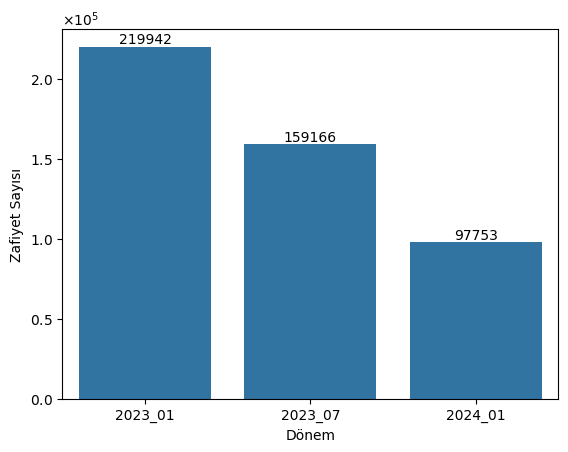
\includegraphics[width=1\linewidth]{images/s2/detected-vulns-by-period.png}
    \caption{Tüm dönemlerdeki tarama araçlarına ait tespit edilen zafiyetler.}\label{fig:detected-vulns-by-period}
\end{figure}

Şekil~\ref{fig:detected-uniq-vulns-by-period} dönemlere göre eşsiz (unique) zafiyet tespitlerini gösterilmektedir. Dönem-1'den Dönem-3'e kadar tüm imajlarda 1138 benzersiz CVE zafiyeti tamamen çözülmüştür.

\begin{figure}
    \centering
    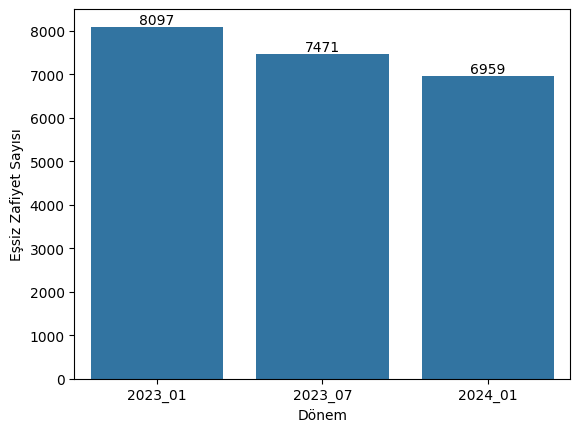
\includegraphics[width=1\linewidth]{images/s2/detected-uniq-vulns-by-period.png}
    \caption{Tüm dönemlerde tespit edilen benzersiz güvenlik açıkları}\label{fig:detected-uniq-vulns-by-period}
\end{figure}

Bu analizden elde edilen sonuçlar, Docker imajlarıın düzenli olarak güncellenmesinin kritik öneminin altını çizmektedir.

\subsection{Şiddet ve Döneme Göre Sonuçlar}\label{subsec:results-severity-and-period}

Şekil~\ref{fig:vuln-severity-period-1} ve tablo~\ref{tab:vuln-severity-period-1} güvenlik açığı tespitlerini önem derecesine göre ayrılmış olarak görülmektedir. Tarama işlemi sırasında, ihmal edilebilir ve bilinmeyen güvenlik açıkları hariç tutulmuştur, çünkü bu güvenlik açıkları önemli bir riske sahip değildir.

\begin{figure}
    \centering
    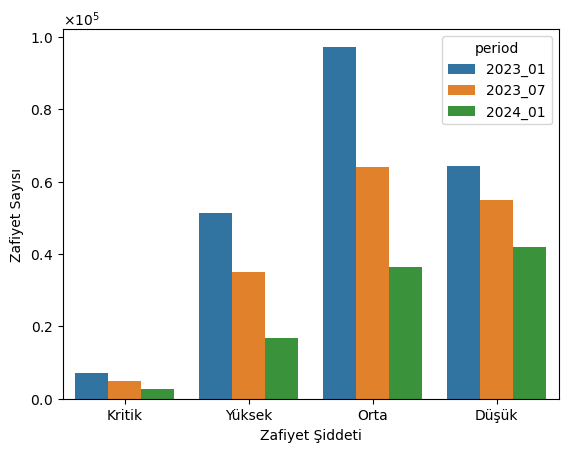
\includegraphics[width=1\linewidth]{images/s2/vuln-severity-period-1.png}
    \caption{Şiddet ve döneme göre sonuçlar}\label{fig:vuln-severity-period-1}
\end{figure}

\begin{table}
    \centering
    \begin{tabular}{ |c|c|c|c|c| }
        \hline
        Dönemler & Düşük & Orta & Yüksek & Kritik \\
        \hline
        Dönem-1 & 64263 & 97244 & 51442 & 6993 \\
        Dönem-2 & 55019 & 64094 & 35110 & 4943 \\
        Dönem-3 & 41802 & 36477 & 16728 & 2746 \\
        \hline
    \end{tabular}
    \caption{Tarama aracına ve şiddete göre tespit edilen güvenlik açıkları.}\label{tab:vuln-severity-period-1}
\end{table}

Kritik güvenlik açıkları en tehlikeli ve ciddi olanlardır, bu da tespit edilmelerini çok önemli kılar, yüksek ciddiyetli güvenlik açıkları kritik olanlardan daha az ciddi olsa da tespit edilmeleri yine de önemlidir. Şekil~\ref{fig:vuln-severity-period-1} ve tablo~\ref{tab:vuln-severity-period-1}'te, tüm dönemlerde güvenlik açığı sayısı zaman içinde azalmaktadır. Kritik ve yüksek güvenlik açıkları için güncel olmayan imajlar, güncellenmiş olanlara kıyasla iki kat daha fazla güvenlik açığı içermektedir.

\begin{figure}
    \centering
    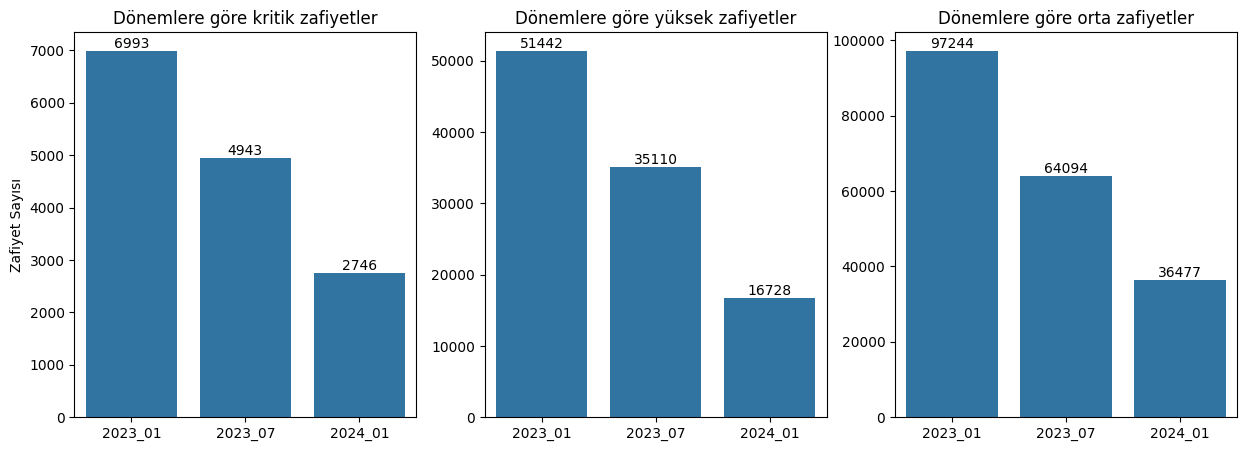
\includegraphics[width=1\linewidth]{images/s2/severity-over-periods.png}
    \caption{Zafiyet şiddetlerinin dönemler içerisindeki dağılımı}\label{fig:severity-over-periods}
\end{figure}

Bu rakamlardan, bir yıllık güncellenmemiş Docker imajlarının güncellenmiş olanlara göre \%154 daha fazla kritik güvenlik açığına sahip olduğunu, altı aylık güncellenmemiş docker imajlarının güncellenmiş olanlara göre \%80 daha fazla kritik güvenlik açığına sahip olduğunu söylenebilir. Benzer şekilde, bir yıllık güncellenmemiş docker imajları güncellenmiş olanlara kıyasla \%207 daha fazla yüksek güvenlik açığına sahipken, altı aylık güncellenmemiş docker imajları \%109 daha fazla yüksek güvenlik açığına sahiptir. Yine benzer şekilde, bir yıllık güncellenmemiş docker imajları güncellenmiş olanlara göre \%166 daha fazla orta düzey güvenlik açığına sahipken, altı aylık güncellenmemiş docker imajları \%75 daha fazla orta düzey güvenlik açığına sahiptir.

% critical p2/p3 180.01 p1/p3 254.66
% high p2/p3 209.89 p1/p3 307.52
% medium p2/p3 175.71 p1/p3 266.59

\subsection{Periyotlar Halinde En Savunmasız Docker İmajları}\label{subsec:most-vuln-images-in-periods}

Docker imajlarındaki yüksek sayıdaki güvenlik açıkları önemli zararlara neden olabilir. Bu nedenle farklı dönemlerdeki en fazla güvenlik açığına sahip olan Docker imajları listelendi. Dönemlere göre güvenlik açığı değişikliklerini gözlemlemek için aynı imajların farklı dönemlerdeki güvenlik açıklarını da tabloya dahil edildi.

Tablo~\ref{tab:most-vuln-images-p1} Dönem-1'e ait en fazla zafiyet sayısına sahip Docker imajları ``circleci/python:3.9.9-buster'', ardından ``apache/superset:2.0.1'' ve sonra ``library/hipache:0.3.1'' olarak gelmektedir. Bunlar Docker Hub'da en çok kullanılan Docker imajlarıdır. Bazı imajların güvenlik açıklarının ``apache/superset'', ``library/haskell'', ``library/perl'' gibi önemli ölçüde azaldığını görebiliriz. İlginçtir ki bazı imajların güvenlik açıkları ``circleci/openjdk'' ve ``library/hipache'' gibi dönemler boyunca artmaktadır. Normal koşullarda daha eski Docker imajları daha fazla güvenlik açığı içermesi gerekir fakat güncel sürümlerde eklenen yeni bağımlılıklar, paketler ve yeni özellikler daha fazla güvenli açığının oluşmasına neden olabilmektedir. Bu durum, yeni Docker imajlarının, eski imajlarda olmayan yeni türde güvenlik zafiyetlerine maruz kalma olasılığını artırmıştır.

\begin{table}
    \centering
    \begin{tabular}{ |c|>{\bfseries}c|c|c| }
        \hline
        Docker İmajı & Dönem-1 & Dönem-2 & Dönem-3 \\
        \hline
        circleci/python  & 4834 & 4834 & 3987 \\
        apache/superset  & 3731 &  927 &  454 \\
        library/hipache  & 3577 & 3577 & 3578 \\
        library/haskell  & 3433 & 2266 & 1866 \\
        library/gazebo   & 3250 &  775 &  907 \\
        circleci/openjdk & 3199 & 3199 & 3367 \\
        library/perl     & 3170 & 2171 &  967 \\
        library/elixir   & 3059 & 2211 & 1032 \\
        library/gcc      & 2978 & 2028 &  968 \\
        cimg/ruby        & 2917 & 2574 &  960 \\
        \hline
    \end{tabular}
    \caption{Dönem-1'deki en zafiyetli docker imajları}\label{tab:most-vuln-images-p1}
\end{table}

Tablo~\ref{tab:most-vuln-images-p2}'de görüldüğü gibi Dönem-2'de ``circleci/python:3.9.9-buster'' hala en zafiyetli Docker imajıdır ve bu imaj önceki dönemden itibaren herhangi bir güvenlik güncellemesi almamıştır. İkinci olarak ``library/hipache:0.3.1'' ve üçüncü olarak ``circleci/openjdk:17-buster'' gelmektedir. Genel olarak çoğu imajın güvenlik açıkları dönemler içinde azalmaktadır.

\begin{table}
    \centering
    \begin{tabular}{ |c|c|>{\bfseries}c|c| }
        \hline
        Docker İmajı & Dönem-1 & Dönem-2 & Dönem-3 \\
        \hline
        circleci/python    & 4834 & 4834 & 3987 \\
        library/hipache    & 3577 & 3577 & 3578 \\
        circleci/openjdk   & 3199 & 3199 & 3367 \\
        library/ros        & 2602 & 2917 &  349 \\
        library/silverpeas & 2808 & 2808 &  725 \\
        cimg/ruby          & 2917 & 2574 &  960 \\
        redash/redash      & 2526 & 2526 & 3878 \\
        library/owncloud   & 2295 & 2295 & 2313 \\
        library/haskell    & 3433 & 2266 & 1866 \\
        library/elixir     & 3059 & 2211 & 1032 \\
        \hline
    \end{tabular}
    \caption{Dönem-2'deki en zafiyetli docker imajları}\label{tab:most-vuln-images-p2}
\end{table}

Tablo~\ref{tab:most-vuln-images-p3}'da görüldüğü gibi Dönem-3 içinde ``atlassian/default-image:latest'' en zafiyetli imajdır, ardından ``circleci/python:latest'' ve üçüncü olarak ``redash/redash:latest'' gelmektedir.

\begin{table}
    \centering
    \begin{tabular}{ |c|c|c|>{\bfseries}c| }
        \hline
        Docker İmajı & Dönem-1 & Dönem-2 & Dönem-3 \\
        \hline
        atlassian/default-image & 1621 & 1266 & 4373 \\
        circleci/python         & 4834 & 4834 & 3987 \\
        redash/redash           & 2526 & 2526 & 3878 \\
        library/hipache         & 3577 & 3577 & 3578 \\
        circleci/openjdk        & 3199 & 3199 & 3367 \\
        library/owncloud        & 2295 & 2295 & 2313 \\
        library/haskell         & 3433 & 2266 & 1866 \\
        library/sl              & 1190 & 1190 & 1721 \\
        library/pypy            & 2532 & 2022 & 1445 \\
        cimg/python             & 2479 & 2039 & 1357 \\
        \hline
    \end{tabular}
    \caption{Dönem-3'deki en zafiyetli docker imajları}\label{tab:most-vuln-images-p3}
\end{table}

Üç tablo göz önünde bulundurulduğunda, bu docker imajlarını kullanmaktan kaçınmanızı öneririz. Mümkünse sıkılaştırılmış (hardened) imajları kullanmayı düşünün.

\subsection{Dönemlerdeki İmaj Kategorileri}\label{subsec:image-categories-in-periods}

Şekil~\ref{fig:image-type-by-periods}'de imaj kategorileri ve tespit edilen güvenlik açıkları görülmektedir. Güncellenmemiş docker imajları güncellenmiş olanlara kıyasla iki kat daha fazla güvenlik açığı içermektedir.

\begin{figure}
    \centering
    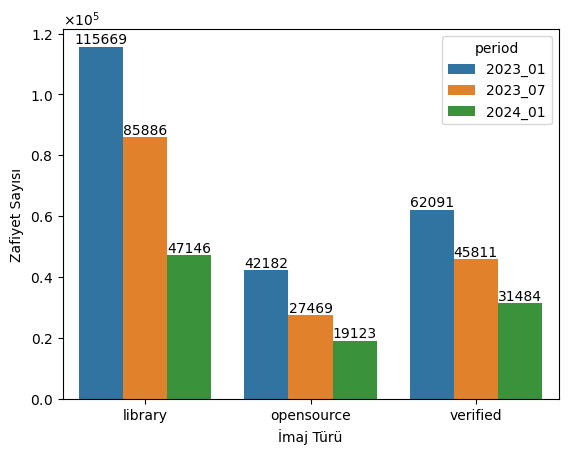
\includegraphics[width=1\linewidth]{images/s2/image-type-by-periods.png}
    \caption{Dönemlere göre imaj türü güvenlik açıkları}\label{fig:image-type-by-periods}
\end{figure}

Güncel olmayan yazılım imajlarının, güncel olanlara kıyasla önemli ölçüde daha fazla güvenlik zaafiyeti içerdiği tespit edildi. Özellikle, bir yıldır güncellenmemiş library imajları, güncel olanlara kıyasla \%145 daha fazla güvenlik açığı taşımaktadır. Bu güvenlik açığı artışı, yalnızca altı ay güncellenmemiş olan library imajları için \%82'ye düşmektedir. Aynı eğilim açık kaynaklı imajlar için de geçerlidir. Bir yıldır güncellenmemiş açık kaynak Docker imajları, güncel sürümlere kıyasla \%120 daha fazla güvenlik açığına maruz kalmaktadır. Bu risk, güncellemelerin yalnızca altı ay gerisinde kalan açık kaynaklı imajlar için \%43 daha fazla güvenlik açığı ile hala önemlidir. Güncellemeleri bir yıl gecikmiş olan verified Docker imajları, güncellenmiş olanlara kıyasla \%97 daha fazla güvenlik açığı taşımaktadır. Sadece altı ay güncellenmemiş verified imajlar için risk daha düşük olsa da \%45'lık bir artış vardır.

Şekil~\ref{fig:image-type-severity}'da gösterildiği gibi, veriler açık bir eğilimi doğrulamaktadır: güncel olmayan yazılım imajları, güncellenmiş benzerlerine kıyasla sürekli olarak daha fazla sayıda güvenlik açığı taşımaktadır. Bu güvenlik açığı farkı, çeşitli imaj türlerinde ve tüm güvenlik açığı şiddetlerinde belirgindir.

\begin{figure}
    \centering
    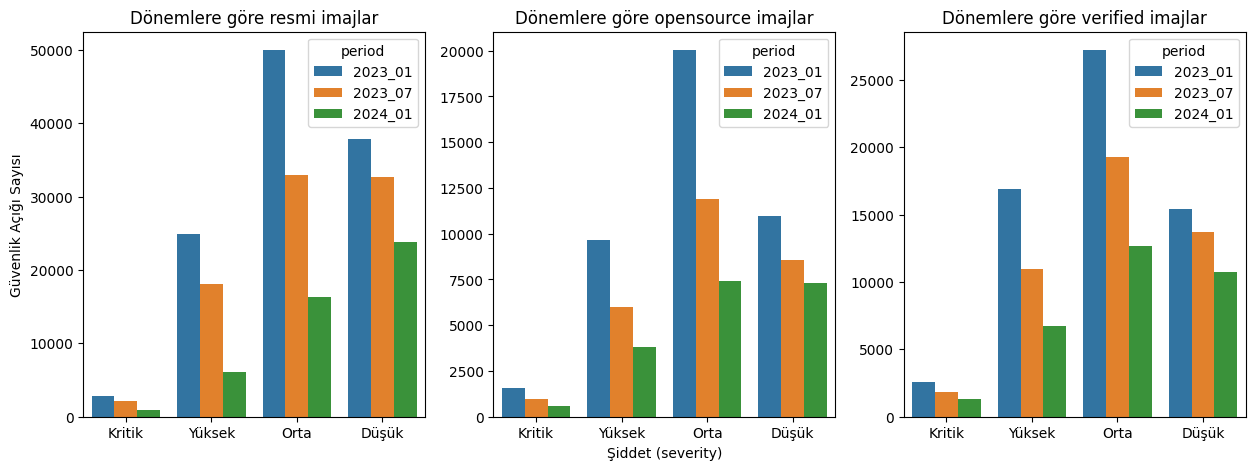
\includegraphics[width=1\linewidth]{images/s2/image-type-severity.png}
    \caption{Zafiyetlerin imaj kategorilerine ve şiddete göre dağılımı.}\label{fig:image-type-severity}
\end{figure}

Bu eğilim, güncel yazılım imajlarını korumanın kritik önemini vurgulamaktadır. Kuruluşlar library, açık kaynaklı ve verified Docker imajlarını güncel tutarak güvenlik açıklarına maruz kalma risklerini önemli ölçüde azaltabilirler.

\subsection{Tespit Edilen En Eski CVE'ler}\label{subsec:detected-oldest-cves}

Tablo~\ref{tab:oldest-cves-count} bölümünde tüm imajlar içerisinde tespit edilen en eski CVE'ler ve bunların tespit sıklıkları listelenmiştir. İlginç bir şekilde, çok eski CVE'ler hala Docker imajlarında bulunabilmektedir.

\begin{table}
    \centering
    \begin{tabular}{ |c|c| }
        \hline
        Zafiyet (CVE) & Tespit Sayısı \\
        \hline
        CVE-1999{-}0236  & 14 \\
        CVE-1999{-}0678  & 12 \\
        CVE-1999{-}1237  & 14 \\
        CVE-1999{-}1412  & 14 \\
        CVE-2001{-}1534  & 143 \\
        CVE-2002{-}1976  & 6 \\
        CVE-2002{-}2439  & 7 \\
        CVE-2003{-}1307  & 143 \\
        CVE-2003{-}1580  & 143 \\
        CVE-2003{-}1581  & 143 \\
        CVE-2004{-}0230  & 118 \\
        CVE-2004{-}0971  & 10 \\
        CVE-2005{-}0406  & 560 \\
        CVE-2005{-}1119  & 16 \\
        CVE-2005{-}2541  & 387 \\
        CVE-2005{-}3660  & 118 \\
        CVE-2006{-}20001 & 77 \\
        CVE-2007{-}0086  & 157 \\
        CVE-2007{-}0450  & 14 \\
        CVE-2007{-}1667  & 3 \\
        \hline
    \end{tabular}
    \caption{Tespit edilen en eski CVE'ler ve tespit sayıları.}\label{tab:oldest-cves-count}
\end{table}

\subsection{İşletim Sistemi İmajları}\label{subsec:os-images}

İşletim Sistemi (OS) imajları, Docker imajlarının büyük çoğunluğu için temel oluşturmaktadır. Python, OpenJDK ve Ruby gibi popüler imajlar, temel olarak OS imajlarından yararlanır. Bu katmanlı yaklaşım, birçok geliştiricinin uygulamaları için temel imajlar üzerine inşa etmesiyle daha da genişlemektedir. Sonuç olarak, bir işletim sistemi imajında bulunan herhangi bir güvenlik açığı, onu miras alan sonraki tüm imajlara yayılabilir. Bu miras zinciri, temel olarak kullanılan işletim sistemi imajlarını korumanın kritik öneminin altını çizmektedir. Zafiyetli bir temel (base) işletim sistemi imajının etkisi geniş ve kapsamlı olabilir. Yaygın olarak kullanılan bir Debian imajında bulunabilecek kritik bir güvenlik açığının bulunduğu bir senaryo düşünün. Bu güvenlik açığı Debian imajının kendisiyle sınırlı kalmayacaktır; aynı zamanda üzerine inşa edilen tüm Python, OpenJDK ve Ruby imajlarında ve hatta potansiyel olarak bu imajlar üzerine inşa edilen uygulamalarda da mevcut olacaktır. Bu zincirleme etki, tek bir güvenlik açığının neden olduğu potansiyel hasarı büyütür.

\begin{figure}
    \centering
    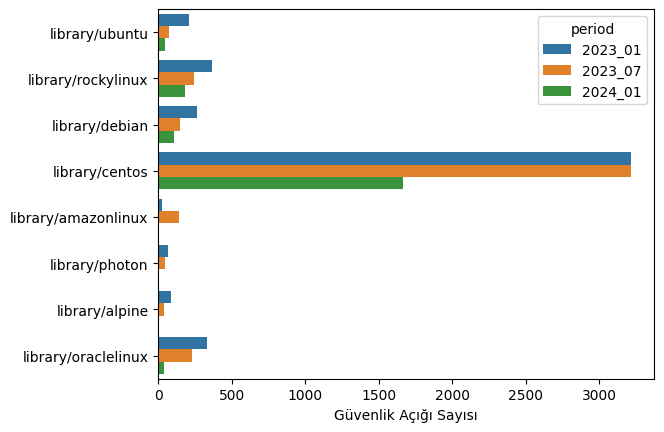
\includegraphics[width=1\linewidth]{images/s2/os-images-by-period.png}
    \caption{OS imajlarına ait zafiyet sayıları.}\label{fig:os-images-by-period}
\end{figure}

\begin{table}
    \centering
    \begin{tabular}{ |c|c|c|c|c| }
        \hline
        İmaj İsmi & Dönem-1 & Dönem-2 & Dönem-3 \\
        \hline
        library/alpine      &   87 &   40 & 4 \\
        library/amazonlinux &   26 &  141 & 6 \\
        library/centos      & 3213 & 3213 & 1667 \\
        library/debian      &  262 &  149 & 104 \\
        library/oraclelinux &  332 &  228 & 42 \\
        library/photon      &   64 &   46 & 0 \\
        library/rockylinux  &  363 &  245 & 182 \\
        library/ubuntu      &  206 &   72 & 46 \\
        \hline
    \end{tabular}
    \caption{İşletim sistemi imajlarında periyotlara göre tespit edilen güvenlik açıkları.}\label{tab:os-images-by-period}
\end{table}

Şekil~\ref{fig:os-images-by-period}'de görüldüğü gibi RHEL tabanlı dağıtımlarda en zafiyetli işletim sistemi docker imajı CentOS'tur. Bunun nedeni, Docker Hub'daki CentOS imajlarının bir yıl içinde herhangi bir güncelleme almamış olmasıdır. Oracle Linux ve Rocky Linux gibi diğer RHEL dağıtımları çok daha az güvenlik açığına sahiptir. Herhangi bir kullanım durumu için, Oracle Linux ve Rocky Linux Docker imajlarını CentOS imajlarına göre tavsiye edilebilir.

Tüm işletim sistemi imajlarında ``library/photon'' ve ``library/alpine'' en güvenli işletim sistemi imajlarından bazılarıdır çünkü Dönem-3'te bu imajların neredeyse sıfır veya birkaç güvenlik açığı vardır. Uygun olan yerlerde Alpine ve Photon docker imajlarını öneririz. Ubuntu Linux çok popüler bir Debian Linux dağıtımıdır, fakat ilginç bir şekilde Ubuntu Debian'dan daha az güvenlik açığına sahiptir. Bunun en temel sebebi olarak Ubuntu imajının Debian'a kıyasla daha az paket ile gelmesi ve daha küçük boyuta sahip olması (Debian 117MB, Ubuntu 76MB) gösterilebilir.

\subsection{Programlama Dili İmajları}\label{subsec:prog-lang-images}

Programlama dili imajları birçok imaj tarafından temel imaj olarak kullanılır ve benzer şekilde birçok geliştirici bu imajları kendi uygulamalarında temel imaj olarak kullanırlar. Örneğin, Django, Flask ve FastAPI web çerçeveleri Python imajını temel imaj olarak kullanır, React, Vue, Nextjs, Express uygulamaları Nodejs'i temel imaj olarak kullanır, Springboot, JSF uygulamaları OpenJDK'yı temel olarak kullanır, Ruby on Rails uygulamaları Ruby imajlarını kullanır, Rust ve Golang uygulamaları uygulamaları oluşturmak/derlemek için Rust ve Golang imajlarını kullanır. Programlama dili imajlarında bulunan herhangi bir güvenlik açığı, bu imajları temel olarak kullanılan bütün Docker imajlarında da ortaya çıkar. Bu da programlama dili imajlarını çok önemli hale getirmektedir.

Şekil~\ref{fig:proglang-by-periods} ve tablo~\ref{tab:proglang-by-periods}'da programlama dillerinin farklı dönemlerdeki güvenlik açıkları listelenmiştir. Güncellenmiş imajların eski imajlara göre çok daha az güvenlik açığı içerdiği gözlemlenebilir.

\begin{figure}
    \centering
    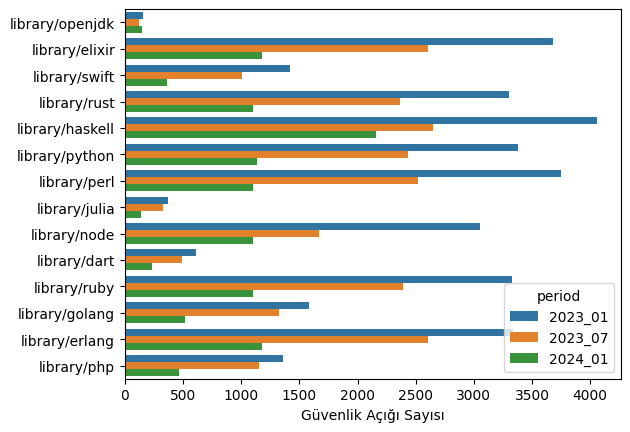
\includegraphics[width=1\linewidth]{images/s2/proglang-by-periods.png}
    \caption{Programlama dili imajlarının zafiyet sayısı.}\label{fig:proglang-by-periods}
\end{figure}

\begin{table}
    \centering
    \begin{tabular}{ |c|c|c|c|c| }
        \hline
        Docker İmajı & Dönem-1 & Dönem-2 & Dönem-3 \\
        \hline
        library/golang  &  159 &  117 &  145 \\
        library/ruby    & 3678 & 2605 & 1178 \\
        library/perl    & 1420 & 1006 &  363 \\
        library/openjdk & 3304 & 2366 & 1102 \\
        library/rust    & 4061 & 2645 & 2155 \\
        library/python  & 3376 & 2434 & 1136 \\
        library/node    & 3751 & 2520 & 1102 \\
        library/erlang  &  372 &  324 &  141 \\
        library/haskell & 3051 & 1664 & 1103 \\
        library/swift   &  613 &  487 &  236 \\
        library/julia   & 3324 & 2394 & 1102 \\
        library/php     & 1583 & 1321 &  520 \\
        library/dart    & 3335 & 2605 & 1178 \\
        library/elixir  & 1357 & 1153 &  461 \\
        \hline
    \end{tabular}
    \caption{Dönemlere göre programlama dili imajlarındaki zafiyetler}\label{tab:proglang-by-periods}
\end{table}

\subsection{Zafiyet Düzeltilme Durumlarına Göre Dağılım}\label{subsec:fix-status}

Her gün yeni güvenlik açıkları keşfedilmekte ve bu güvenlik açıklarını yamamak için sürekli olarak güncellemeler yayınlanmaktadır. Şekil~\ref{fig:vuln-fix-status}'da güvenlik açığı düzeltilme durumu bulunabilir. Dönem-1'deki güvenlik açıklarının çoğunun ``fixed'' statüsüne sahip olduğuna dikkat edin, yani güncellemeler uygulanarak bu zafiyetler tamamiyle giderilebilir. Aynı şey Dönem-2 için de söylenebilir. Ayrıca, ``not-fixed'' ve ``wont-fix'' zafiyet değişikliklerinin ``fixed'' durumuna kıyasla önemli ölçüde değişmediği söylenebilir.

\begin{figure}
    \centering
    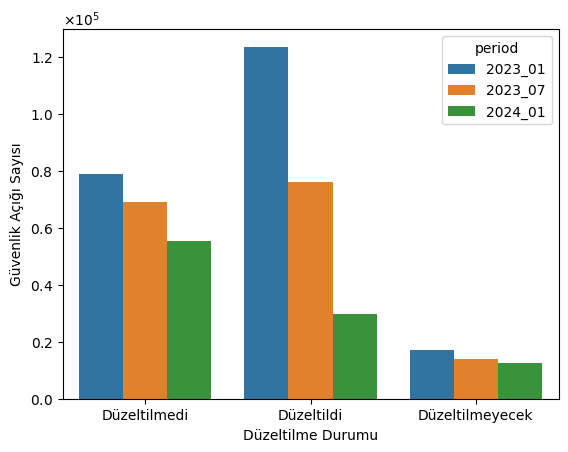
\includegraphics[width=1\linewidth]{images/s2/vuln-fix-status.png}
    \caption{Güvenlik Açığı Düzeltme Durumu}\label{fig:vuln-fix-status}
\end{figure}

\chapter{Sonuçlar ve Öneriler}\label{ch:kapanis}

Docker imajlarının kullanımı, bilgi teknolojileri alanında uygulama ve yazılım geliştirmeyi kolaylaştırmıştır. Aynı zamanda yeni güvenlik problemlerini de beraberinde getirmiştir. Bu tez çalışmasında Docker imajlarındaki güvenlik açıklarının zaman içerisindeki değişiminin incelenmesi ve araştırılmasının yanı sıra mevcut Docker imaj tarama araçlarının etkinliği de ele alınmaktadır.

Tezin ilk aşamasında Docker Hub'da resmi, doğrulanmış ve açık kaynak olarak kategorize edilen en popüler 439 Docker imajı üzerinde bir tarama gerçekleştirilmiştir. Tarama sonuçlarını değerlendirmek için güvenlik açığı tespit isabet oranı metriği kullanılmış ve CVSS güvenlik açığı puanlama sistemine dayalı yeni bir metrik önerilmiştir. Bu metrikler, imaj tarama araçlarının etkinliği hakkında bilgi sağlamış ve güncel Docker imajlarındaki güvenlik açıklarını ortaya çıkarmıştır. Kapsamı artırmak için bu iki metrikten elde edilen sonuçların karşılaştırmalı bir analizi yapılmıştır.

Çalışmanın ikinci aşamasında Docker Hub'dan alınan resmi, doğrulanmış ve açık kaynak olarak kategorize edilen en popüler 364 Docker imajı ve bu imajların 3 farklı sürümleri üzerinde bir tarama yapılmıştır. Tarama sonuçları, işletim sistemi docker imajlarının güvenlik açığı değişiklikleri, programlama dili docker imajları, kategoriye göre imajlar, dönemler arası zafiyet sayısı değişikliği vb.\ gibi farklı perspektiflerden değerlendirmek için kullanılmıştır. Bu metrikler Docker imajların güvenlik durumu hakkında fikir vermiş ve en güncel Docker imajlarındaki güvenlik risklerini ortaya çıkarmıştır.

Tez sonuçları şu şekilde listelenebilir:

\begin{itemize}
    \item Taramalar sonucunda Trivy'nin en fazla sayıda zafiyet tespit ettiği, Grype'ın ise en fazla sayıda benzersiz zafiyet tespit ediği görülmüştür.
    \item En iyi tarama aracı Docker imajlarındaki önemli sayıda güvenlik açığını tespit edemediği ve diğer araçların daha da az performans gösterdiği gözlemlenmiştir.
    \item Risk tabanlı olarak önerilen VSM ve SVSM metrikleri ile güvenlik açıklarının riskleri ön plana çıkartılmıştır.
    % ----------------------------------------------------------
    \item Bir yıl süre ile güncellenmemiş docker imajlarının güncellenmiş olanlara kıyasla yaklaşık 2 katı zafiyet barındırmaktadır.
    \item Bir yıl süre ile güncellenmemiş docker imajlarının 1138 benzersiz CVE barındırabildiği tespit edilmiştir.
    \item Dönemler içindeki en zafiyetli docker imajları belirlenmiş ve bu imajların güncellendiği taktirde zafiyetlerin büyük bir kısmının düzeltilebildiği görülmüştür.
    \item CVE-2001-1534 gibi 2000'li yıllardan kalma bazı zafiyetlerin hala docker imajlarında bulunabildiği tespit edilmiştir.
    \item Desteği kesilmiş CentOS gibi işletim sistemi imajları çok sayıda zafiyet içerebilmektedir. Bu imajlar yerine Alpine ve Photon gibi imajlar tercih edilerek zafiyet sayısı azaltılabilir.
    \item Programlama dillerine ait imajların güncellenmedikleri taktirde 2 veya 3 kat daha fazla zafiyet içerebildiği görülmüştür.
    \item Taramalar sonucunda tespit edilen zafiyetlerin çoğunun güncellemelerin uygulanması ile düzeltilebileceği tespit edilmiştir.
\end{itemize}

Bu tez göstermiştir ki, Docker imajlarının güvenliği büyük ölçüde güncellemeler ve uygun tarama araçlarının kullanılmasıyla artırılabilir. Docker imaj güvenliği bulut tabanlı teknolojilerin ve yazılım geliştirme süreçlerinin önemli bir parçası olmaya devam edecektir. Bu alandaki çalışmaların devam etmesi, imaj güvenliğini daha da ileriye taşıyacak ve daha güvenli yazılımların oluşturulmasına yardımcı olacaktır.

\chapter{Veri Erişilebilirliği}\label{sec:data-availability}

Bu tez kapsamında oluşturulan veriseti, bu alanda daha farklı çalışmaları teşvik etmek için paylaşılmıştır. Verisetimiz, çalışmada kullanılan Bash ve Python betik dosyaları, Ipynb dosyaları, tarama sonuçlarının JSON hali ile birlikte GitHub depomuzda paylaşılmıştır. Bu kaynaklara aşağıdaki bağlantıdan erişilebilir:

\begin{lstlisting}
https://github.com/hatsat32/yltez
\end{lstlisting}
